\documentclass[a4paper]{article}
\usepackage{a4wide}
\usepackage[pdftex]{graphicx}
\usepackage{color}
\usepackage{amsmath,amssymb,amsthm}
\usepackage{tikz}
\usetikzlibrary{arrows}
\usepackage{verbatim}

\definecolor{olivegreen}{cmyk}{0.64,0,0.95,0.40}
\definecolor{rawsienna}{cmyk}{0,0.72,1,0.45}
\definecolor{lightgreen}{rgb}{0.85,1.0,0.85}

\newcommand{\GREENYELLOW}[1]{{\color{greenyellow}#1}}
\newcommand{\YELLOW}[1]{{\color{yellow}#1}}
\newcommand{\YLW}[1]{{\color{yellow}#1}}
\newcommand{\GOLDENROD}[1]{{\color{goldenrod}#1}}
\newcommand{\DANDELION}[1]{{\color{dandelion}#1}}
\newcommand{\APRICOT}[1]{{\color{apricot}#1}}
\newcommand{\PEACH}[1]{{\color{peach}#1}}
\newcommand{\MELON}[1]{{\color{melon}#1}}
\newcommand{\YELLOWORANGE}[1]{{\color{yelloworange}#1}}
\newcommand{\ORANGE}[1]{{\color{orange}#1}}
\newcommand{\BURNTORANGE}[1]{{\color{burntorange}#1}}
\newcommand{\BITTERSWEET}[1]{{\color{bittersweet}#1}}
\newcommand{\REDORANGE}[1]{{\color{redorange}#1}}
\newcommand{\MAHOGANY}[1]{{\color{mahogany}#1}}
\newcommand{\MAROON}[1]{{\color{maroon}#1}}
\newcommand{\BRICKRED}[1]{{\color{brickred}#1}}
\newcommand{\RED}[1]{{\color{red}#1}}
\newcommand{\ORANGERED}[1]{{\color{orangered}#1}}
\newcommand{\RUBINERED}[1]{{\color{rubinered}#1}}
\newcommand{\WILDSTRAWBERRY}[1]{{\color{wildstrawberry}#1}}
\newcommand{\SALMON}[1]{{\color{salmon}#1}}
\newcommand{\CARNATIONPINK}[1]{{\color{carnationpink}#1}}
\newcommand{\MAGENTA}[1]{{\color{magenta}#1}}
\newcommand{\VIOLETRED}[1]{{\color{violetred}#1}}
\newcommand{\RHODAMINE}[1]{{\color{rhodamine}#1}}
\newcommand{\MULBERRY}[1]{{\color{mulberry}#1}}
\newcommand{\REDVIOLET}[1]{{\color{redviolet}#1}}
\newcommand{\FUCHSIA}[1]{{\color{fuchsia}#1}}
\newcommand{\LAVENDER}[1]{{\color{lavender}#1}}
\newcommand{\THISTLE}[1]{{\color{thistle}#1}}
\newcommand{\ORCHID}[1]{{\color{orchid}#1}}
\newcommand{\DARKORCHID}[1]{{\color{darkorchid}#1}}
\newcommand{\PURPLE}[1]{{\color{purple}#1}}
\newcommand{\PLUM}[1]{{\color{plum}#1}}
\newcommand{\VIOLET}[1]{{\color{violet}#1}}
\newcommand{\ROYALPURPLE}[1]{{\color{royalpurple}#1}}
\newcommand{\BLUEVIOLET}[1]{{\color{blueviolet}#1}}
\newcommand{\PERIWINKLE}[1]{{\color{periwinkle}#1}}
\newcommand{\CADETBLUE}[1]{{\color{cadetblue}#1}}
\newcommand{\CORNFLOWERBLUE}[1]{{\color{cornflowerblue}#1}}
\newcommand{\MIDNIGHTBLUE}[1]{{\color{midnightblue}#1}}
\newcommand{\NAVYBLUE}[1]{{\color{navyblue}#1}}
\newcommand{\ROYALBLUE}[1]{{\color{royalblue}#1}}
\newcommand{\BLU}[1]{{\color{blue}#1}}
\newcommand{\BLUE}[1]{{\color{blue}#1}}
\newcommand{\CERULEAN}[1]{{\color{cerulean}#1}}
\newcommand{\CYAN}[1]{{\color{cyan}#1}}
\newcommand{\PROCESSBLUE}[1]{{\color{processblue}#1}}
\newcommand{\SKYBLUE}[1]{{\color{skyblue}#1}}
\newcommand{\TURQUOISE}[1]{{\color{turquoise}#1}}
\newcommand{\TEALBLUE}[1]{{\color{tealblue}#1}}
\newcommand{\AQUAMARINE}[1]{{\color{aquamarine}#1}}
\newcommand{\BLUEGREEN}[1]{{\color{bluegreen}#1}}
\newcommand{\EMERALD}[1]{{\color{emerald}#1}}
\newcommand{\JUNGLEGREEN}[1]{{\color{junglegreen}#1}}
\newcommand{\SEAGREEN}[1]{{\color{seagreen}#1}}
\newcommand{\GREEN}[1]{{\color{green}#1}}
\newcommand{\FORESTGREEN}[1]{{\color{forestgreen}#1}}
\newcommand{\PINEGREEN}[1]{{\color{pinegreen}#1}}
\newcommand{\LIMEGREEN}[1]{{\color{limegreen}#1}}
\newcommand{\YELLOWGREEN}[1]{{\color{yellowgreen}#1}}
\newcommand{\SPRINGGREEN}[1]{{\color{springgreen}#1}}
\newcommand{\OLIVEGREEN}[1]{{\color{olivegreen}#1}}
\newcommand{\OLG}[1]{{\color{olivegreen}#1}}
\newcommand{\RAWSIENNA}[1]{{\color{rawsienna}#1}}
\newcommand{\SEPIA}[1]{{\color{sepia}#1}}
\newcommand{\BROWN}[1]{{\color{brown}#1}}
\newcommand{\TAN}[1]{{\color{tan}#1}}
\newcommand{\GRAY}[1]{{\color{gray}#1}}
\newcommand{\LGRAY}[1]{{\color{gray!40}#1}}
\newcommand{\WHITE}[1]{{\color{white}#1}}
\newcommand{\BLACK}[1]{{\color{black}#1}}

\newcommand{\bbm}       {\left[\begin{matrix}}
\newcommand{\ebm}       {\end{matrix}\right]}
\newcommand{\bsm}       {\left[\begin{smallmatrix}}
\newcommand{\esm}       {\end{smallmatrix}\right]}
\newcommand{\bpm}       {\begin{pmatrix}}
\newcommand{\epm}       {\end{pmatrix}}
\newcommand{\bcf}[2]{\left(\begin{array}{c}{#1}\\{#2}\end{array}\right)}

\newcommand{\adj}       {\operatorname{adj}}
\newcommand{\ann}       {\operatorname{ann}}
\newcommand{\diag}      {\operatorname{diag}}
\newcommand{\img}       {\operatorname{img}}
\newcommand{\rnk}       {\operatorname{rank}}
\newcommand{\sgn}       {\operatorname{sgn}}
\newcommand{\spn}       {\operatorname{span}}
\newcommand{\trc}       {\operatorname{trace}}

\newcommand{\pp}{\hphantom{+}}
\newcommand{\tm}{\times}
\newcommand{\sse}{\subseteq}
\newcommand{\st}{\;|\;}
\newcommand{\sm}{\setminus}
\newcommand{\iffa}      {\Leftrightarrow}
\newcommand{\xra}{\xrightarrow}
\newcommand{\xla}{\xleftarrow}

\newcommand{\half}{\tfrac{1}{2}}

\newcommand{\N}         {{\mathbb{N}}}
\newcommand{\Z}         {{\mathbb{Z}}}
\newcommand{\Q}         {{\mathbb{Q}}}
\newcommand{\R}         {{\mathbb{R}}}
\newcommand{\C}         {{\mathbb{C}}}

\newcommand{\va}        {\mathbf{a}}
\newcommand{\vb}        {\mathbf{b}}
\newcommand{\vc}        {\mathbf{c}}
\newcommand{\vd}        {\mathbf{d}}
\newcommand{\ve}        {\mathbf{e}}
\newcommand{\vf}        {\mathbf{f}}
\newcommand{\vg}        {\mathbf{g}}
\newcommand{\vh}        {\mathbf{h}}
\newcommand{\vi}        {\mathbf{i}}
\newcommand{\vj}        {\mathbf{j}}
\newcommand{\vk}        {\mathbf{k}}
\newcommand{\vl}        {\mathbf{l}}
\newcommand{\vm}        {\mathbf{m}}
\newcommand{\vn}        {\mathbf{n}}
\newcommand{\vo}        {\mathbf{o}}
\newcommand{\vp}        {\mathbf{p}}
\newcommand{\vq}        {\mathbf{q}}
\newcommand{\vr}        {\mathbf{r}}
\newcommand{\vs}        {\mathbf{s}}
\newcommand{\vt}        {\mathbf{t}}
\newcommand{\vu}        {\mathbf{u}}
\newcommand{\vv}        {\mathbf{v}}
\newcommand{\vw}        {\mathbf{w}}
\newcommand{\vx}        {\mathbf{x}}
\newcommand{\vy}        {\mathbf{y}}
\newcommand{\vz}        {\mathbf{z}}

\newcommand{\vA}        {\mathbf{A}}
\newcommand{\vB}        {\mathbf{B}}
\newcommand{\vC}        {\mathbf{C}}
\newcommand{\vD}        {\mathbf{D}}
\newcommand{\vE}        {\mathbf{E}}
\newcommand{\vF}        {\mathbf{F}}
\newcommand{\vG}        {\mathbf{G}}
\newcommand{\vH}        {\mathbf{H}}
\newcommand{\vI}        {\mathbf{I}}
\newcommand{\vJ}        {\mathbf{J}}
\newcommand{\vK}        {\mathbf{K}}
\newcommand{\vL}        {\mathbf{L}}
\newcommand{\vM}        {\mathbf{M}}
\newcommand{\vN}        {\mathbf{N}}
\newcommand{\vO}        {\mathbf{O}}
\newcommand{\vP}        {\mathbf{P}}
\newcommand{\vQ}        {\mathbf{Q}}
\newcommand{\vR}        {\mathbf{R}}
\newcommand{\vS}        {\mathbf{S}}
\newcommand{\vT}        {\mathbf{T}}
\newcommand{\vU}        {\mathbf{U}}
\newcommand{\vV}        {\mathbf{V}}
\newcommand{\vW}        {\mathbf{W}}
\newcommand{\vX}        {\mathbf{X}}
\newcommand{\vY}        {\mathbf{Y}}
\newcommand{\vZ}        {\mathbf{Z}}

\newcommand{\al}        {\alpha}
\newcommand{\bt}        {\beta} 
\newcommand{\gm}        {\gamma}
\newcommand{\dl}        {\delta}
\newcommand{\ep}        {\epsilon}
\newcommand{\zt}        {\zeta}
\newcommand{\et}        {\eta}
\newcommand{\tht}       {\theta}
\newcommand{\io}        {\iota}
\newcommand{\kp}        {\kappa}
\newcommand{\lm}        {\lambda}
\newcommand{\ph}        {\phi}
\newcommand{\ch}        {\chi}
\newcommand{\ps}        {\psi}
\newcommand{\rh}        {\rho}
\newcommand{\sg}        {\sigma}
\newcommand{\om}        {\omega}

\newcommand{\Gm}        {\Gamma}
\newcommand{\Dl}        {\Delta}

\newcommand{\CA}        {\mathcal{A}}
\newcommand{\CB}        {\mathcal{B}}
\newcommand{\CC}        {\mathcal{C}}
\newcommand{\CD}        {\mathcal{D}}
\newcommand{\CE}        {\mathcal{E}}
\newcommand{\CF}        {\mathcal{F}}
\newcommand{\CG}        {\mathcal{G}}
\newcommand{\CH}        {\mathcal{H}}
\newcommand{\CI}        {\mathcal{I}}
\newcommand{\CJ}        {\mathcal{J}}
\newcommand{\CK}        {\mathcal{K}}
\newcommand{\CL}        {\mathcal{L}}
\newcommand{\CM}        {\mathcal{M}}
\newcommand{\CN}        {\mathcal{N}}
\newcommand{\CO}        {\mathcal{O}}
\newcommand{\CP}        {\mathcal{P}}
\newcommand{\CQ}        {\mathcal{Q}}
\newcommand{\CR}        {\mathcal{R}}
\newcommand{\CS}        {\mathcal{S}}
\newcommand{\CT}        {\mathcal{T}}
\newcommand{\CU}        {\mathcal{U}}
\newcommand{\CV}        {\mathcal{V}}
\newcommand{\CW}        {\mathcal{W}}
\newcommand{\CX}        {\mathcal{X}}
\newcommand{\CY}        {\mathcal{Y}}
\newcommand{\CZ}        {\mathcal{Z}}


\newcommand{\ov}        {\overline}
\newcommand{\ip}[1]     {\langle #1\rangle}
\renewcommand{\ss}      {\scriptstyle}

\renewcommand{\:}       {\colon}

\newcommand{\barmat}[2]{\left[\begin{array}{c|c}\!\!\raisebox{0pt}[0.45cm][0.35cm]{$#1$} & \raisebox{0pt}[0.45cm][0.35cm]{$#2$}\!\!\end{array}\right]}

\newcommand{\eqpair}[4]{\begin{array}{rl} #1 &= #2 \\ #3 &= #4\end{array}}

\newcommand{\han}[1]{\begin{CJK*}{UTF8}{zhsong}\BLUE{#1}\end{CJK*}}
\newcommand{\bhan}[1]{(\begin{CJK*}{UTF8}{zhsong}\BLUE{#1}\end{CJK*})}

\newcommand{\EMPH}[1]{\emph{\RED{#1}}}
\newcommand{\DEFN}[1]{\emph{\PURPLE{#1}}}
\newcommand{\VEC}[1]    {\mathbf{#1}}

\newcommand{\ghost}{{\tiny $\color[rgb]{1,1,1}.$}}

\newcommand{\reminderbar}{\par\medskip\par\hrule\par\medskip\par}

\newcommand{\uc}{\uncover}

\newcommand{\bbox}[1]{
\[ \mbox{\begin{tikzpicture}%
   \draw(0,0) node[draw,thick,olivegreen,rectangle] {\color{black} #1};%
  \end{tikzpicture}} \]
}

\newcommand{\cbox}[1]{
\begin{center}\begin{tikzpicture}%
   \draw(0,0) node[draw,thick,olivegreen,rectangle] {\color{black} #1};%
\end{tikzpicture}\end{center}
}


\newcounter{probcounter}
\newcounter{marksassigned}
\newcounter{marksawarded}
\newcounter{totalmarks}

\newcommand{\mrks}[1]{%
\addtocounter{marksassigned}{#1}%
\addtocounter{totalmarks}{#1}%
\textbf{(#1 marks)}}
\newcommand{\mrk}{%
\addtocounter{marksassigned}{1}%
\addtocounter{totalmarks}{1}%
\textbf{(1 mark)}}
\newcommand{\mks}[1]{%
\addtocounter{marksawarded}{#1}%
\textbf{\color{red}[#1]}}
\newcommand{\mk}{\mks{1}}

\newenvironment{problem}{
\stepcounter{probcounter}
\setcounter{marksawarded}{0}
\bigskip\par\noindent\textbf{(\arabic{probcounter})}
}{
\typeout{Q\arabic{probcounter}: \arabic{marksassigned} marks assigned}
\setcounter{marksassigned}{0}
}

\def\SOLS{1}
\ifx\SOLS\undefined
\newenvironment{solution}{\comment}{\endcomment}
\else
\newenvironment{solution}{
{\bigskip\par\noindent \bf Solution:}}{
\newpage
\typeout{Q\arabic{probcounter}: \arabic{marksawarded} marks awarded}
}
\fi

\newcommand{\printtotalmarks}{%
\typeout{Total assigned: \arabic{totalmarks} marks}%
}

\newcommand{\sct}{\section}

\newcommand{\np}{\newpage}

\begin{document}

\begin{center}
 {\Huge Methods for Differential Equations \\(NTech) \\ All exam questions}
\end{center}
\vspace{4ex}

\section*{Question 1}

\begin{problem} % 2013-14 Q1
 \begin{itemize}
  \item[(i)]
   Suppose we have four linear systems with
   properties described below.  In each case, find the type of
   equilibrium at the origin. \mrks{8}
   \begin{itemize}
    \item The matrix for system A has characteristic polynomial $t^2+t+1$.
    \item System B corresponds to the following point in the
     $(\tau,\dl)$ plane:
     \begin{center}
      \begin{tikzpicture}[scale=2.5]
       \draw (-1.2,-0.3) rectangle (1.2,1.2);
       \draw[thick,cyan] (-1,0) -- (0,0);
       \draw[thick,orange,->] (0,0) -- (1,0);
       \draw[thick,olivegreen,->] (0,0) -- (0,1);
       \draw[thick,blue,smooth] (-1,1) -- (-0.9,0.81) -- (-0.8,0.64) --
         (-0.7,0.49) -- (-0.6,0.36) -- (-0.5,0.25) -- (-0.4,0.16) --
         (-0.3,0.09) -- (-0.2,0.04) -- (-0.1,0.01) -- (0,0);
       \draw[thick,red,smooth] (1,1) -- (0.9,0.81) -- (0.8,0.64) --
         (0.7,0.49) -- (0.6,0.36) -- (0.5,0.25) -- (0.4,0.16) --
         (0.3,0.09) -- (0.2,0.04) -- (0.1,0.01) -- (0,0);
       \draw(0,1) node[anchor=south]{$\ss\dl$};
       \draw(1,0) node[anchor=west]{$\ss\tau$};
       \fill[black] (0.8,-0.1) circle(0.02);
      \end{tikzpicture}
     \end{center}
    \item The solution for system~C involves a term $e^{4t}\cos(7t)$
    \item Both eigenvalues for system~D are real and negative.
   \end{itemize}
  \item[(ii)] Consider the system
   $\bbm \dot{x}\\\dot{y}\ebm=A\bbm x\\ y\ebm$, where
   $A=\bbm 110 & -10 \\ 100 & 0 \ebm$.
   \begin{itemize}
    \item[(a)] Find the eigenvalues of $A$.  \mrks{4}
    \item[(b)] Find a matrix $P$ (depending on $t$) such that
     $\dot{P}=AP$, and $P=I$ when $t=0$.  \mrks{6}
    \item[(c)] Find the solution to the system for which $x=0$ and
     $y=90$ when $t=0$. \mrks{3}
   \end{itemize}
  \item[(iii)] Which of the following matrices corresponds to a system
   with a clockwise centre at the origin? \mrks{4}
   \[ \bbm  1 &  2 \\  2 &  1 \ebm \qquad
      \bbm  1 & -2 \\  2 & -1 \ebm \qquad
      \bbm  2 & -1 \\  1 & -2 \ebm \qquad
      \bbm  1 &  2 \\ -2 & -1 \ebm \qquad
      \bbm  2 &  1 \\ -1 & -2 \ebm \qquad
      \bbm -1 &  2 \\  2 & -1 \ebm
   \]
 \end{itemize}
\end{problem} 
\begin{solution}\leavevmode
 \textbf{All this is similar to questions in the lectures and on the
  problem sheets.}
 \begin{itemize}
  \item[(i)]
   \begin{itemize}
    \item The eigenvalues for system~A are
     $(-1\pm\sqrt{1-4})/2=-\half\pm\half\sqrt{3}i$.  These are complex
     with negative real part, so the system is a stable focus. \mks{2}
    \item The $(\tau,\dl)$ point for~B lies below the horizontal axis,
     so $\dl<0$, so the system is a saddle. \mks{2}
    \item The solution for~C involves 
     \[ e^{4t}\cos(7t)=\half(e^{(4+7i)t}+e^{(4-7i)t}). \]
     This means that the eigenvalues must be $4\pm 7i$, which are
     complex with positive real part, so the system is an unstable
     focus. \mks{2}
    \item As the eigenvalues for~D are real and negative, it is a stable
     node. \mks{2}
   \end{itemize}
  \item[(ii)] 
   \begin{itemize}
    \item[(a)] The trace and determinant are $\tau=110$ and
     $\dl=1000$ \mks{2}, so 
     \[ \sqrt{\tau^2-4\dl}=\sqrt{12100-4000}=\sqrt{8100}=90. \]
     Thus, the eigenvalues are $(110\pm 90)/2$, which gives $\lm_1=10$
     and $\lm_2=100$. \mks{2}
    \item[(b)] The simplest approach is to use the standard formula 
     \[ P = (\lm_2-\lm_1)^{-1}((e^{\lm_2t}-e^{\lm_1t})A + 
                               (\lm_2e^{\lm_1t}-\lm_1e^{\lm_2t})I). 
        \mks{3}
     \]
     In the present case, this becomes
     \begin{align*}
      P &= \frac{1}{90}\left((e^{100t}-e^{10t})
                              \bbm 110 & -10 \\ 100 & 0 \ebm + 
                             (100e^{10t}-10e^{100t})
                              \bbm 1 & 0 \\ 0 & 1 \ebm\right) \\
        &= \frac{1}{90}\bbm 
            110(e^{100t}-e^{10t}) + (100e^{10t}-10e^{100t}) & 
            -10(e^{100t}-e^{10t}) \\
            100(e^{100t}-e^{10t}) & 
            100e^{10t}-10e^{100t}
           \ebm  \\
        &= \frac{1}{90}\bbm 100 e^{100t} - 10  e^{10t} &
                            -10 e^{100t} + 10  e^{10t} \\
                            100 e^{100t} - 100 e^{10t} &
                            100 e^{100t} - 10  e^{10t}
                       \ebm. \mks{3}
     \end{align*}
     Alternatively, we can use the diagonalisation method.  For that,
     we must find the eigenvectors of $A$.  We first note that
     $A-10I=\bbm 100&-10\\100 & -10\ebm$, so the vector
     $v_1=\bbm 1\\10\ebm$ is an eigenvector of eigenvalue $\lm_1=10$.
     Similarly, we have $A-100I=\bbm 10&-10\\100&-100\ebm$, so the
     vector $v_1=\bbm 1\\ 1\ebm$ is an eigenvector of eigenvalue
     $\lm_2=100$.  It follows that $A=VDV^{-1}$, where 
     \[ D = \bbm \lm_1&0 \\ 0&\lm_2\ebm = \bbm 10 & 0 \\ 0& 100 \ebm \]
     and
     \[ V = \barmat{v_1}{v_2} = \bbm 1 & 1 \\ 10 & 1 \ebm 
        \hspace{4em}
        V^{-1} = -\frac{1}{9} \bbm 1 & -1 \\ -10 & 1 \ebm.
     \]
     This in turn gives $P=VEV^{-1}$, where
     \[ E = \bbm e^{\lm_1 t} & 0 \\ 0 & e^{\lm_2t} \ebm 
          = \bbm e^{10t} & 0 \\ 0 & e^{100t} \ebm.
     \]
     One can check that this gives the same answer as before.
    \item[(iii)] The relevant solution is 
     \[ \bbm x \\ y \ebm = P \bbm x_0\\ y_0\ebm  \mk = 
         \frac{1}{90}\bbm 100 e^{100t} - 10  e^{10t} &
                          -10 e^{100t} + 10  e^{10t} \\
                          100 e^{100t} - 100 e^{10t} &
                          100 e^{100t} - 10  e^{10t}
                     \ebm
                     \bbm 0 \\ 90 \ebm \mk =
         \bbm -10 e^{100t} + 10  e^{10t} \\
              100 e^{100t} - 10  e^{10t} \ebm \mk
     \]
   \end{itemize}
  \item[(iii)] Consider a matrix $A=\bbm a&b\\ c&d\ebm$ with
   $\tau=a+b$ and $\dl=ad-bc$.  This corresponds to a centre if
   $\tau=0$ and $\dl>0$; if so, then the rotation is clockwise
   if $c<0<b$ and anticlockwise if $b<0<c$ \mks{2}.  Only the 4th and 5th
   matrices in the list have $c<0$.  The 4th one has $\dl=3$, and the
   5th has $\dl=-3$, and both have $\tau=0$.  It follows that the 4th
   matrix $\bbm 1&2\\-2&-1\ebm$ is the only one that gives an
   clockwise centre \mks{2}.
 \end{itemize}
\end{solution}

\begin{problem} % 2013-14 R Q1
 \begin{itemize}
  \item[(i)]
   Suppose we have four linear systems with
   properties described below.  In each case, find the type of
   equilibrium at the origin. \mrks{8}
   \begin{itemize}
    \item The matrix for system A has one positive eigenvalue and one negative eigenvalue.
    \item System B corresponds to the following point in the
     $(\tau,\dl)$ plane:
     \begin{center}
      \begin{tikzpicture}[scale=2.5]
       \draw (-1.2,-0.3) rectangle (1.2,1.2);
       \draw[thick,cyan] (-1,0) -- (0,0);
       \draw[thick,orange,->] (0,0) -- (1,0);
       \draw[thick,olivegreen,->] (0,0) -- (0,1);
       \draw[thick,blue,smooth] (-1,1) -- (-0.9,0.81) -- (-0.8,0.64) --
         (-0.7,0.49) -- (-0.6,0.36) -- (-0.5,0.25) -- (-0.4,0.16) --
         (-0.3,0.09) -- (-0.2,0.04) -- (-0.1,0.01) -- (0,0);
       \draw[thick,red,smooth] (1,1) -- (0.9,0.81) -- (0.8,0.64) --
         (0.7,0.49) -- (0.6,0.36) -- (0.5,0.25) -- (0.4,0.16) --
         (0.3,0.09) -- (0.2,0.04) -- (0.1,0.01) -- (0,0);
       \draw(0,1) node[anchor=south]{$\ss\dl$};
       \draw(1,0) node[anchor=west]{$\ss\tau$};
       \fill[black] (-0.2,0.8) circle(0.02);
      \end{tikzpicture}
     \end{center}
    \item The solution for system~C involves $e^{-11t}$ and $e^{-111t}$. 
    \item The matrix for system~D has characteristic polynomial $t^2+10t+100$.
   \end{itemize}
  \item[(ii)] Consider the system
   $\bbm \dot{x}\\\dot{y}\ebm=A\bbm x\\ y\ebm$, where
   $A=\bbm 16 & -25 \\ 13 & -20 \ebm$.
   \begin{itemize}
    \item[(a)] Find the eigenvalues of $A$.  \mrks{4}
    \item[(b)] Find a matrix $P$ (depending on $t$) such that
     $\dot{P}=AP$, and $P=I$ when $t=0$.  \mrks{6}
    \item[(c)] Find the solution to the system for which $x=25$ and
     $y=18$ when $t=0$. \mrks{3}
   \end{itemize}
  \item[(iii)] Which of the following matrices corresponds to a system
   with an anticlockwise focus at the origin? \mrks{4}
   \[ 
     \bbm -2 & 2 \\ 2 & -1 \ebm \qquad
     \bbm  1 & 2 \\ 2 &  2 \ebm \qquad
     \bbm  1 &-2 \\-2 & -2 \ebm \qquad
     \bbm  2 &-2 \\ 2 & -1 \ebm \qquad
     \bbm  2 &-1 \\ 2 & -2 \ebm \qquad
     \bbm  2 & 2 \\-2 & -1 \ebm
   \]
 \end{itemize}
\end{problem} 
\begin{solution}\leavevmode
 \textbf{All this is similar to questions in the lectures and on the
  problem sheets.}
 \begin{itemize}
  \item[(i)]
   \begin{itemize}
    \item Any linear system with one positive eigenvalue and one
     negative eigenvalue is a saddle. \mks{2}
    \item The $(\tau,\dl)$ point for~B lies above the parabola, so
     $\tau^2-4\dl<0$, so we have a focus.  It is stable because
     $\tau<0$. \mks{2} 
    \item The solution for~C involves $e^{-11t}$ and $e^{-111t}$, so
     the eigenvalues must be $-11$ and $-111$.  These are both real
     and negative, so we have a stable node. \mks{2}
    \item Recall that the characteristic polynomial is always
     $t^2-\tau t+\dl$.  Thus, for~D we have $\tau=-10<0$ and
     $\dl=100>0$, so $\tau^2-4\dl=-300<0$.  We therefore have a stable
     focus, just as in system~B. \mks{2}
   \end{itemize}
  \item[(ii)] 
   \begin{itemize}
    \item[(a)] The trace and determinant are $\tau=16-20=-4$ and
     $\dl=16\tm(-20)-13\tm(-25)=5$ \mks{2}, so 
     \[ \sqrt{\tau^2-4\dl}=\sqrt{16-20}=\sqrt{-4}=2i. \]
     Thus, the eigenvalues are $(-4\pm 2i)/2$, which gives $\lm_1=-2-i$
     and $\lm_2=-2+i$. \mks{2}
    \item[(b)] The simplest approach is to use the standard formula 
     \[ P = e^{\lm t}(\cos(\om t)I + \om^{-1}\sin(\om t)(A - \lm I))
        \mks{3}
     \]
     In the present case, we have $\lm=-2$ and $\om=1$ so
     \begin{align*}
      P &= e^{-2t}\left(
            \cos(t) \bbm 1 & 0 \\ 0 & 1 \ebm +
            \sin(t) \bbm 18 & -25 \\ 13 & -18 \ebm
           \right) \\
        &= \bbm 
            e^{-2t}(\cos(t)+18\sin(t)) &
            -25 e^{-2t}\sin(t) \\
            13 e^{-2t}\sin(t) &
            e^{-2t}(\cos(t)-18\sin(t))
           \ebm. \mks{3}
     \end{align*}
    \item[(c)] The relevant solution is 
     \begin{align*}
       \bbm x \\ y \ebm = P \bbm x_0\\ y_0\ebm  \mk & = 
           \bbm 
            e^{-2t}(\cos(t)+18\sin(t)) &
            -25 e^{-2t}\sin(t) \\
            13 e^{-2t}\sin(t) &
            e^{-2t}(\cos(t)-18\sin(t))
           \ebm
           \bbm 25 \\ 18 \ebm \\
           &=
           e^{-2t} \bbm 
            25\cos(t) + 450\sin(t) - 450\sin(t) \\ 
            325\sin(t) + 18\cos(t) - 324\sin(t)
           \ebm = 
           e^{-2t} \bbm 
            25\cos(t) \\ 
            \sin(t) + 18\cos(t)
           \ebm.\mks{2}
     \end{align*}
   \end{itemize}
  \item[(iii)] The matrices in the question are as follows:
   \[ \def\VP{\vphantom{\bbm 0\\0\\0\ebm}}
      \begin{array}{|r|c|r|r|r|l|} \hline 
       && \tau & \dl & \tau^2-4\dl & \text{ type } \\ \hline
       \VP A_1 & \bbm -2 & 2 \\ 2 & -1 \ebm & -3 & -2 & 17 & \text{ saddle } \\ \hline
       \VP A_2 & \bbm  1 & 2 \\ 2 &  2 \ebm &  3 & -2 & 17 & \text{ saddle } \\ \hline
       \VP A_3 & \bbm  1 &-2 \\-2 & -2 \ebm & -1 & -6 & 25 & \text{ saddle } \\ \hline
       \VP A_4 & \bbm  2 &-2 \\ 2 & -1 \ebm &  1 &  2 & -7 & \text{ anticlockwise unstable focus } \\ \hline
       \VP A_5 & \bbm  2 &-1 \\ 2 & -2 \ebm &  0 & -2 &  8 & \text{ saddle } \\ \hline
       \VP A_6 & \bbm  2 & 2 \\-2 & -1 \ebm &  1 &  2 & -7 & \text{ clockwise unstable focus } \\ \hline
      \end{array}
   \]
   Most of them have $\dl<0$ so they are saddles.  Matrices $A_4$ and
   $A_6$ have $\tau^2-4\dl<0$ so they are foci (and $\tau>0$ so they
   are unstable).  In $A_4$ the bottom left entry is positive, so the
   rotation is anticlockwise.  In $A_6$ the bottom left entry is
   negative, so the rotation is clockwise.  Thus, the only
   anticlockwise focus is $A_4$.\mks{4}
 \end{itemize}
\end{solution}

\begin{problem} % 2014-15 Q1
 \begin{itemize}
%  \item[(iv)] Consider the equations 
%   \[ \dot{x}=ax+by \hspace{4em} \dot{y}=bx+ay, \]
%   where $a$ and $b$ are nonzero real constants.  Give examples to 
%   show that the system can have a saddle, a stable node or an
%   unstable node at $(0,0)$, depending on the values of $a$ and $b$,
%   but it cannot have a focus or centre.
  \item[(i)] Consider the equations 
   \[ \dot{x} = (a+b)x + 2by \hspace{4em}
      \dot{y} = -bx + (a-b)y, 
   \]
   where $a$ and $b$ are nonzero real constants.  Show that the system
   always has a focus at $(0,0)$.  Give examples to show that the
   focus can be stable or unstable, and clockwise or anticlockwise,
   depending on the values of $a$ and $b$. \mrks{7}
  \item[(ii)] Consider the functions 
   \[ x = e^t + 2 e^{2t} \hspace{4em} y = e^t - 2 e^{2t}, \]
   and the vector function $u=\bbm x \\ y \ebm$.  Find a constant
   matrix $A$ such that $\dot{u}=Au$. \mrks{6}
  \item[(iii)] For each of the following matrices $A_k$, find a matrix
   $P_k$ (depending on $t$) such that $\dot{P}_k=AP_k$, and $P_k=I$
   when $t=0$. \mrks{12}
   \[ A_0 = \bbm 1 & 1 \\  1 & 1 \ebm \qquad
      A_1 = \bbm 1 & 1 \\  0 & 1 \ebm \qquad      
      A_2 = \bbm 1 & 1 \\ -1 & 1 \ebm.
   \]
 \end{itemize}
\end{problem} 
\begin{solution}\leavevmode
 \begin{itemize}
%  \item[(iv)]
%   The corresponding matrix is $A=\bbm a&b\\ b&a\ebm$ \mk, with trace
%   $\tau=2a$ \mk and determinant $\dl=a^2-b^2$ \mk.  This gives
%   \[ \tau^2-4\dl = 4a^2 - 4(a^2-b^2) = 4b^2 > 0. \mk \]
%   For a focus or centre we would have $\tau^2-4\dl<0$, so we cannot
%   have a focus or centre \mk.  If $a^2<b^2$ then $\dl<0$ and we have a
%   saddle; for example, this occurs when $a=1$ and $b=2$ \mk.  If $a<0$
%   and $a^2>b^2$ then we have a stable node; for example, this happens
%   when $a=-2$ and $b=-1$ \mk.  If $a>0$ and $a^2>b^2$ then we have an
%   unstable node; for example, this happens when $a=2$ and $b=1$ \mk.
%
%   All this could alternatively be discussed in terms of the
%   eigenvalues of $A$, which are
%   \[ (\tau\pm\sqrt{\tau^2-4\dl})/2 = 
%      (2a\pm 2b)/2 = a+b \text{ and } a-b.
%   \] 
  \item[(i)] \textbf{Students have seen many questions like this where
   the matrices have numerical entries, but only a few where the
   matrices have symbolic entries.} \\
   The corresponding matrix is $A=\bbm a+b&2b\\ -b&a-b\ebm$ \mk, with trace
   $\tau=2a$ and determinant
   \[ \dl = (a+b)(a-b) - 2b.(-b) = a^2-b^2 + 2b^2 = a^2+b^2 \mk. \]
   This gives
   \[ \tau^2-4\dl = 4a^2 - 4(a^2+b^2) = -4b^2 < 0, \mk \]
   so we have a focus or centre \mk.  However, we have $\tau=2a$ and
   $a\neq 0$ by assumption so we cannot have a centre, and we must
   instead have a focus \mk.  If $a<0$ then $\tau<0$ so the focus is
   stable; similarly, if $a>0$ then the focus is unstable \mk.  The
   direction of rotation is controlled by the bottom left entry in
   $A$, which is $-b$.  If $b<0$ then $-b>0$ so the rotation is
   anticlockwise, but if $b>0$ then the rotation is clockwise \mk.
  \item[(ii)] \textbf{This is unseen.}\\
   Consider a matrix $A=\bbm a&b\\ c&d\ebm$.  We then have 
   \begin{align*}
    \dot{u} &= \bbm e^t + 4e^{2t} \\ e^t - 4 e^{2t} \ebm \mk \\
    Au &= \bbm a & b \\ c & d \ebm
          \bbm e^t + 2 e^{2t} \\ e^t - 2 e^{2t} \ebm 
        = \bbm (a+b) e^t + (2a-2b) e^{2t} \\
               (c+d) e^t + (2c-2d) e^{2t} \ebm \mk
   \end{align*}
   To get $\dot{u}=Au$, we must have $a+b=c+d=1$ and $2a-2b=4$ and
   $2c-2d=-4$ \mks{2}.  These equations can easily be solved to give $a=d=3/2$
   and $b=c=-1/2$, so 
   \[ A = \frac{1}{2} \bbm 3 & -1 \\ -1 & 3 \ebm. \mks{2} \]
  \item[(iii)] \textbf{This is standard.  The students have been told
    that they need to memorise the relevant formulae.}\\
   All three matrices $A_k$ have trace $\tau=2$, and the
   determinants are $0,1$ and $2$.  The corresponding values of
   $\tau^2-4\dl$ are $4$, $0$ and $-4$.  
   \begin{itemize}
    \item[(a)] For $A_0$, the eigenvalues are $(2\pm\sqrt{4})/2$,
     which gives $\lm_1=0$ and $\lm_2=2$ (both real) \mk.  The standard
     formula in this context is
     \[ P = \frac{1}{\lm_2-\lm_1}\left(
             (\lm_2e^{\lm_1t}-\lm_1e^{\lm_2t})I + 
             (e^{\lm_2t}-e^{\lm_1t})A
            \right). \mks{2}
     \]
     In the present case, this becomes
     \begin{align*}
      P_0 &= \frac{1}{2}\left(
             (2e^0-0e^{2t})I + (e^{2t}-e^0)A_0
            \right)
          = \frac{1}{2}\left(
             \bbm 2 & 0 \\ 0 & 2 \ebm + 
             (e^{2t}-1) \bbm 1 & 1 \\ 1 & 1 \ebm
            \right) \\
          &= \frac{1}{2}\bbm e^{2t} + 1 & e^{2t} - 1 \\
                            e^{2t} - 1 & e^{2t} + 1 \ebm. \mk
     \end{align*}
    \item[(b)] For $A_1$, the eigenvalues are $(2\pm\sqrt{0})/2$, so
     $\lm=1$ is a repeated eigenvalue \mk.  The standard formula in this
     context is 
     \[ P = e^{\lm t}(I + t(A-\lm I)). \mks{2} \]
     In the present case, this becomes
     \[ P_1 = e^t \left(\bbm 1 & 0 \\ 0 & 1 \ebm + 
                        t \bbm 0 & 1 \\ 0 & 0 \ebm\right)
            = \bbm e^t & t\,e^t \\ 0 & e^t \ebm. \mk 
     \]
    \item[(c)] For $A_2$, the eigenvalues are $(2\pm\sqrt{-4})/2$,
     which gives $1\pm i$ \mk.  The standard formula in this context is 
     \[ P = e^{\lm t}\left(\cos(\om t) I +
               \om^{-1}\sin(\om t)(A - \lm I)\right). \mks{2}
     \]
     In the present case we have $\lm=\om=1$, giving 
     \[ P = e^t\left(\cos(t)\bbm 1 & 0 \\ 0 & 1\ebm + 
                     \sin(t)\bbm 0 & 1 \\ -1 & 0\ebm\right) = 
          e^t \bbm \cos(t) & \sin(t) \\ -\sin(t) & \cos(t) \ebm. \mk
     \]
   \end{itemize}
 \end{itemize}
\end{solution}

\begin{problem} % 2014-15 R Q1
 \begin{itemize}
  \item[(i)]
   Suppose we have four linear systems with
   properties described below.  In each case, find the type of
   equilibrium at the origin. \mrks{8}
   \begin{itemize}
    \item The matrix for system A has two complex eigenvalues with positive real part.
    \item System B corresponds to the following point in the
     $(\tau,\dl)$ plane:
     \begin{center}
      \begin{tikzpicture}[scale=2.5]
       \draw (-1.2,-0.3) rectangle (1.2,1.2);
       \draw[thick,cyan] (-1,0) -- (0,0);
       \draw[thick,orange,->] (0,0) -- (1,0);
       \draw[thick,olivegreen,->] (0,0) -- (0,1);
       \draw[thick,blue,smooth] (-1,1) -- (-0.9,0.81) -- (-0.8,0.64) --
         (-0.7,0.49) -- (-0.6,0.36) -- (-0.5,0.25) -- (-0.4,0.16) --
         (-0.3,0.09) -- (-0.2,0.04) -- (-0.1,0.01) -- (0,0);
       \draw[thick,red,smooth] (1,1) -- (0.9,0.81) -- (0.8,0.64) --
         (0.7,0.49) -- (0.6,0.36) -- (0.5,0.25) -- (0.4,0.16) --
         (0.3,0.09) -- (0.2,0.04) -- (0.1,0.01) -- (0,0);
       \draw(0,1) node[anchor=south]{$\ss\dl$};
       \draw(1,0) node[anchor=west]{$\ss\tau$};
       \fill[black] (0.3,-0.15) circle(0.02);
      \end{tikzpicture}
     \end{center}
    \item The solution for system~C involves $e^{-\pi t}\cos(3t)$. 
    \item The matrix for system~D has characteristic polynomial $t^2+5t-50$.
   \end{itemize}
  \item[(ii)] Consider the equations 
   \[ \dot{x}=ax+by \hspace{4em} \dot{y}=bx+ay, \]
   where $a$ and $b$ are nonzero real constants.  Give examples to 
   show that the system can have a saddle, a stable node or an
   unstable node at $(0,0)$, depending on the values of $a$ and $b$,
   but it cannot have a focus or centre. \mrks{8}
  \item[(iii)] Which of the following matrices corresponds to a system
   with an anticlockwise focus at the origin? \mrks{5}
   \[ 
     \bbm -2 & 2 \\ 2 & -1 \ebm \qquad
     \bbm  1 & 2 \\ 2 &  2 \ebm \qquad
     \bbm  1 &-2 \\-2 & -2 \ebm \qquad
     \bbm  2 &-2 \\ 2 & -1 \ebm \qquad
     \bbm  2 &-1 \\ 2 & -2 \ebm \qquad
     \bbm  2 & 2 \\-2 & -1 \ebm
   \]
  \item[(iv)] Let $A$ be a $2\tm 2$ matrix with real eigenvalues $\lm_1$
   and $\lm_2$, where $\lm_1\neq\lm_2$.  Give a formula for a matrix
   $P(t)$ satisfying $P(0)=I$ and $\dot{P}=AP$.  \mrks{4}
 \end{itemize}
\end{problem} 
\begin{solution}\leavevmode
 \textbf{All this is similar to questions in the lectures,
  problem sheets and past papers.}
 \begin{itemize}
  \item[(i)]
   \begin{itemize}
    \item The system must be an unstable focus. \mks{2}
    \item The $(\tau,\dl)$ point for~B lies below the $\tau$-axis, so
     $\dl<0$, so we have a saddle. \mks{2} 
    \item The solution for~C involves $e^{-\pi t}\cos(3t)$, so the
     eigenvalues must be $-\pi\pm 3i$.  These are complex with strictly
     negative real part, so we have a stable focus. \mks{2}
    \item Recall that the characteristic polynomial is always
     $t^2-\tau t+\dl$.  Thus, for~D we have $\tau=-5<0$ and
     $\dl=-50<0$.  As $\dl<0$, this is a saddle. \mks{2}
   \end{itemize}
  \item[(ii)]
   The corresponding matrix is $A=\bbm a&b\\ b&a\ebm$ \mk, with trace
   $\tau=2a$ \mk and determinant $\dl=a^2-b^2$ \mk.  This gives
   \[ \tau^2-4\dl = 4a^2 - 4(a^2-b^2) = 4b^2 > 0. \mk \]
   For a focus or centre we would have $\tau^2-4\dl<0$, so we cannot
   have a focus or centre \mk.  If $a^2<b^2$ then $\dl<0$ and we have a
   saddle; for example, this occurs when $a=1$ and $b=2$ \mk.  If $a<0$
   and $a^2>b^2$ then we have a stable node; for example, this happens
   when $a=-2$ and $b=-1$ \mk.  If $a>0$ and $a^2>b^2$ then we have an
   unstable node; for example, this happens when $a=2$ and $b=1$ \mk.

   All this could alternatively be discussed in terms of the
   eigenvalues of $A$, which are
   \[ (\tau\pm\sqrt{\tau^2-4\dl})/2 = 
      (2a\pm 2b)/2 = a+b \text{ and } a-b.
   \] 
  \item[(iii)] The matrices in the question are as follows:
   \[ \def\VP{\vphantom{\bbm 0\\0\\0\ebm}}
      \begin{array}{|r|c|r|r|r|l|} \hline 
       && \tau & \dl & \tau^2-4\dl & \text{ type } \\ \hline
       \VP A_1 & \bbm -2 & 2 \\ 2 & -1 \ebm & -3 & -2 & 17 & \text{ saddle } \\ \hline
       \VP A_2 & \bbm  1 & 2 \\ 2 &  2 \ebm &  3 & -2 & 17 & \text{ saddle } \\ \hline
       \VP A_3 & \bbm  1 &-2 \\-2 & -2 \ebm & -1 & -6 & 25 & \text{ saddle } \\ \hline
       \VP A_4 & \bbm  2 &-2 \\ 2 & -1 \ebm &  1 &  2 & -7 & \text{ anticlockwise unstable focus } \\ \hline
       \VP A_5 & \bbm  2 &-1 \\ 2 & -2 \ebm &  0 & -2 &  8 & \text{ saddle } \\ \hline
       \VP A_6 & \bbm  2 & 2 \\-2 & -1 \ebm &  1 &  2 & -7 & \text{ clockwise unstable focus } \\ \hline
      \end{array}
   \]
   Most of them have $\dl<0$ so they are saddles.  Matrices $A_4$ and
   $A_6$ have $\tau^2-4\dl<0$ so they are foci (and $\tau>0$ so they
   are unstable).  In $A_4$ the bottom left entry is positive, so the
   rotation is anticlockwise.  In $A_6$ the bottom left entry is
   negative, so the rotation is clockwise.  Thus, the only
   anticlockwise focus is $A_4$.\mks{5}
  \item[(iv)] The standard formula is 
   \[ P = \frac{1}{\lm_2-\lm_1}\left(
           (\lm_2e^{\lm_1t}-\lm_1e^{\lm_2t})I + (e^{\lm_2t}-e^{\lm_1t})A
          \right) \mks{4}
  \]
 \end{itemize}
\end{solution}

\begin{problem} % 2015-16 Q1
 \begin{itemize}
  \item[(i)] Consider the matrix 
   \[ P = e^{2t} \bbm 
       7\cos(3t) + \sin(3t) & 4\cos(3t) - 3\sin(3t) \\
        \cos(3t) + \sin(3t) & \cos(3t)
      \ebm.
   \]
   Find a matrix $A$ such that $\dot{P}=AP$.  Is $P$ the fundamental
   solution for $A$? \mrks{6}
  \item[(ii)] For any number $a\in\R$, we put 
   \[ Q(a) = \bbm a/2 & 1/8 \\ a^2-1 & a/2\ebm. \]
   Find numbers $a_1,\dotsc,a_5$ such that 
   \begin{itemize}
    \item $Q(a_1)$ has a stable node at the origin.
    \item $Q(a_2)$ has a stable focus at the origin.
    \item $Q(a_3)$ has a centre at the origin.
    \item $Q(a_4)$ has an unstable focus at the origin.
    \item $Q(a_5)$ has an unstable node at the origin.
   \end{itemize}
   For $Q(a_3)$, is the rotation clockwise or anticlockwise?  For
   $Q(a_5)$, what are the eigenvalues? \mrks{10}
  \item[(iii)] Consider the matrix 
   \[ A=\bbm 0 & \ln(2)\ln(3) \\ -1 & \ln(6) \ebm. \]
   Find the eigenvalue and eigenvectors.  Find a matrix $P$ depending
   on $t$ such that $\dot{P}=AP$, and $P=I$ when $t=0$. \mrks{9}
 \end{itemize}
\end{problem}
\begin{solution}
 \begin{itemize}
  \item[(i)] \textbf{This is a minor variation on a standard theme.}
   Write $s=\sin(3t)$ and $c=\cos(3t)$ and
   $A=\bbm m&n\\p&q\ebm$.  We then have
   \begin{align*}
    \dot{P}
     &= 2e^{2t} \bbm 7c+s & 4c-3s \\ c+s & c \ebm + 
         e^{2t} \bbm -21s+3c & -12s-9c \\ -3s+3c & -3s \ebm \\
     &=  e^{2t} \bbm 17c -19s & -c-18s \\ 5c-s & 2c-3s \ebm \mk \\
    AP &= e^{2t}\bbm m&n\\p&q\ebm
            \bbm 7c+s & 4c-3s \\ c+s & c \ebm \\
     &= e^{2t} \bbm (7m+n)c+(m+n)s & (4m+n)c-3ms \\
                    (7p+q)c+(p+q)s & (4p+q)c-3ps \ebm \mk
   \end{align*}
   We therefore want 
   \begin{align*}
    7m+n &= 17 & m+n &= -19 \\
    4m+n &= -1 & -3m &= -18 \\
    7p+q &=  5 & p+q &=  -1 \\
    4p+q &=  2 & -3p &=  -3. \mk
   \end{align*}
   These are easily solved to give $m=6$ and $n=-25$ and $p=1$ and
   $q=-2$, so $A=\bbm 6&-25 \\ 1&-2\ebm$ \mks{2}.  If $P$ was the fundamental
   solution for $A$ then we would not only have $\dot{P}=AP$, but also
   $P=I$ when $t=0$.  In fact we have $P=\bbm 7&4\\1&1\ebm$ when
   $t=0$, so $P$ is not the fundamental solution. \mk
  \item[(ii)] \textbf{Students have seen similar problems.}
   For the matrix $Q(a)$ we have
   \begin{align*}
    \tau &= a/2 + a/2 = a \mk \\
    \dl  &= (a/2)^2 - (a^2-1)/8 = (a^2+1)/8 > 0  \\
    \tau^2-4\dl &= a^2 - (a^2+1)/2 = (a^2-1)/2. \mk
   \end{align*}
   \begin{itemize}
    \item For a stable node we need $\tau<0$ and $\dl>0$ and
     $\tau^2-4\dl>0$, so $a<0$ and $a^2>1$.  We can therefore take
     $a_1=-3$. \mk
    \item For a stable focus we need $\tau<0$ and $\dl>0$ and
     $\tau^2-4\dl<0$, so $a<0$ and $a^2<1$.  We can therefore take
     $a_2=-1/2$. \mk
    \item For a centre we need $\tau=0$ and $\dl>0$; the only
     possibility is to take $a_3=0$. \mk
    \item For an unstable focus we need $\tau>0$ and $\dl>0$ and
     $\tau^2-4\dl<0$, so $a>0$ and $a^2<1$.  We can therefore take
     $a_4=1/2$. \mk
    \item For an unstable node we need $\tau>0$ and $\dl>0$ and
     $\tau^2-4\dl>0$, so $a>0$ and $a^2>1$.  We can therefore take
     $a_5=3$. \mk 
   \end{itemize}
   The matrix $Q(a_3)$ is $\bbm 0&1/8 \\ -1&0 \ebm$.  As the bottom
   left entry is negative and the top right entry is positive, we see
   that the rotation is clockwise. \mk The matrix $Q(a_5)$ has $\tau=3$
   and $\tau^2-4\dl=(3^2-1)/2=4$ so the eigenvalues are
   \[ \lm_1,\lm_2 = (\tau\pm\sqrt{\tau^2-4\dl})/2
       = (3\pm 2)/2 = 1/2,\;5/2. \mks{2}
   \]
  \item[(iii)] \textbf{This is a standard problem.}
   We have $\tau=0+\ln(6)=\ln(2)+\ln(3)$ \mk and 
   \[ \dl = 0 \tm \ln(6) - (-1)\tm\ln(2)\ln(3) = \ln(2)\ln(3). \mk \]
   This gives 
   \[ \chi_A(t)=t^2-\tau t+\dl=t^2-(\ln(2)+\ln(3))t+\ln(2)\ln(3)
       = (t-\ln(2))(t-\ln(3)),
   \]
   so the eigenvalues are $\lm_1=\ln(2)$ and $\lm_2=\ln(3)$. \mk For an
   eigenvector $u_1=\bbm p\\ q\ebm$ of eigenvalue $\ln(2)$, we need
   $(A-\ln(2)I)u_2=0$, or equivalently 
   \[ \bbm -\ln(2) & \ln(2)\ln(3) \\ -1 & \ln(3) \ebm
        \bbm p\\ q\ebm = \bbm 0 \\ 0 \ebm.
   \]
   This reduces to $p=\ln(3)q$, so we can take
   $u_1=\bbm\ln(3)\\1\ebm$. \mk  Similarly, we can take
   $u_2=\bbm\ln(2)\\1\ebm$. \mk This gives
   \begin{align*}
    U &= [u_1|u_2] = \bbm \ln(3) & \ln(2) \\ 1 & 1\ebm \mk \\
    U^{-1} &= \frac{1}{\ln(3)-\ln(2)} 
              \bbm 1&-\ln(2) \\ -1&\ln(3) \ebm \\
    D &= \bbm \lm_1 & 0 \\ 0 & \lm_2 \ebm 
       = \bbm \ln(2) & 0 \\ 0 & \ln(3) \ebm \mk \\
    e^{tD} &= \bbm e^{t\ln(2)} & 0 \\ 0 & e^{t\ln(3)} \ebm
            = \bbm 2^t & 0 \\ 0 & 3^t \ebm \\
    P &= U e^{tD} U^{-1} \mk 
       = \frac{1}{\ln(3)-\ln(2)} 
         \bbm \ln(3) & \ln(2) \\ 1 & 1 \ebm 
         \bbm 2^t & 0 \\ 0 & 3^t \ebm 
         \bbm 1&-\ln(2) \\ -1&\ln(3) \ebm \\
      &= \frac{1}{\ln(3)-\ln(2)}  
         \bbm \ln(3)2^t-\ln(2)3^t & \ln(2)\ln(3)(3^t-2^t) \\
              2^t-3^t & 3^t\ln(3) - 2^t\ln(2) \ebm. \mk
   \end{align*}
 \end{itemize}
\end{solution}

\begin{problem} % 2015-16 R Q1
 \begin{itemize}
  \item[(i)] Draw a diagram of the $(\tau,\dl)$-plane, and show which
   regions correspond to saddles, stable nodes, unstable nodes, stable
   foci and unstable foci. \mrks{5}
  \item[(ii)] For any constant $a\in\R$, we can consider the system
   $S_a$ given by the following equations:
   \begin{align*}
    \dot{x} &= x+2y \\
    \dot{y} &= -2x+(a-1)y.
   \end{align*}
   Draw a diagram to show the points corresponding to $S_a$ in the
   $(\tau,\dl)$-plane.  For which values of $a$ does $S_a$ have a
   saddle, stable node, unstable node, stable focus or unstable focus
   at the origin? \mrks{13}
  \item[(iii)] In the cases where $S_a$ has a focus at the origin, is
   the rotation clockwise or anticlockwise? \mrks{2}
  \item[(iv)] Consider the matrix $A=\bbm a+b & -bc \\ b/c & a-b\ebm$.
   Find a matrix $P$ depending on $t$ such that $\dot{P}=AP$, and
   $P=I$ when $t=0$.  \mrks{5}
 \end{itemize}
\end{problem} 
\begin{solution}\leavevmode
 \begin{itemize}
  \item[(i)] The diagram is as follows:\mks{5}
   \begin{center}
    \begin{tikzpicture}[scale=4]
     \draw[thick,cyan] (-1.2,0) -- (0,0);
     \draw[thick,orange,->] (0,0) -- (1.2,0);
     \draw[thick,olivegreen,->] (0,0) -- (0,1);
     \draw[thick,blue,smooth] (-1,1) -- (-0.9,0.81) -- (-0.8,0.64) --
       (-0.7,0.49) -- (-0.6,0.36) -- (-0.5,0.25) -- (-0.4,0.16) --
       (-0.3,0.09) -- (-0.2,0.04) -- (-0.1,0.01) -- (0,0);
     \draw[thick,red,smooth] (1,1) -- (0.9,0.81) -- (0.8,0.64) --
       (0.7,0.49) -- (0.6,0.36) -- (0.5,0.25) -- (0.4,0.16) --
       (0.3,0.09) -- (0.2,0.04) -- (0.1,0.01) -- (0,0);
     \draw(0,1) node[anchor=south]{$\dl$};
     \draw(1,1) node[anchor=south]{$\tau^2-4\dl=0$};
     \draw(1.2,0) node[anchor=west]{$\tau$};
     \draw( 0.4,0.9) node{$\ss \tau>0,\;\tau^2-4\dl<0$};
     \draw( 0.4,0.8) node{$\ss \text{unstable focus}$};
     \draw(-0.4,0.9) node{$\ss \tau<0,\;\tau^2-4\dl<0$};
     \draw(-0.4,0.8) node{$\ss \text{stable focus}$};
     \draw( 0.8,0.2) node{$\ss \tau>0,\;\dl>0,\;\tau^2-4\dl>0$};
     \draw( 0.8,0.1) node{$\ss \text{unstable node}$};
     \draw(-0.8,0.2) node{$\ss \tau<0,\;\dl>0,\;\tau^2-4\dl>0$};
     \draw(-0.8,0.1) node{$\ss \text{stable node}$};
     \draw( 0.0,-0.1) node{$\ss \dl<0$};
     \draw( 0.0,-0.2) node{$\ss \text{saddle}$};
    \end{tikzpicture}
   \end{center}
  \item[(ii)] The system $S_a$ corresponds to the matrix
   $A_a=\bbm 1&2\\-2&a-1\ebm$ with $\tau=a$ \mk and 
   \[ \dl = 1\tm(a-1) - 2\tm (-2) = a+3, \mk \]
   which gives 
   \[ \tau^2-4\dl = a^2-4a-12 = (a+2)(a-6). \mk \]
   Thus:
   \begin{itemize}
    \item When $a<-3$ we have $\dl<0$ and so the system has a saddle.
    \item When $-3<a<-2$ we have $\tau<0$ and $\dl>0$ and
     $\tau^2-4\dl>0$ so the system has a stable node.
    \item When $-2<a<0$ we have $\tau<0$ and $\dl>0$ and
     $\tau^2-4\dl<0$ so the system has a stable focus.
    \item When $0<a<6$ we have $\tau>0$ and $\dl>0$ and
     $\tau^2-4\dl<0$ so the system has an unstable focus.
    \item When $a>6$ we have $\tau>0$ and $\dl>0$ and
     $\tau^2-4\dl>0$ so the system has an unstable node. \mks{5}
   \end{itemize}
   The corresponding points lie on the line $\dl=\tau+3$, which can be
   illustrated as follows: \mks{5}
   \begin{center}
    \begin{tikzpicture}[scale=0.5]
     \draw[thick,cyan] (-8.0,0.0) -- ( 0.0,0.0);
     \draw[thick,orange,->] (0.0,0.0) -- (8.0,0.0);
     \draw[thick,olivegreen,->] (0,0) -- (0,10);
     \draw[thick,blue,smooth,domain=-6.32:0,variable=\x] plot({\x},{0.25*\x*\x});
     \draw[thick,red ,smooth,domain=0:6.32 ,variable=\x] plot({\x},{0.25*\x*\x});
     \draw[black] (-5,-2) -- (7,10);
     \draw[black,dotted] (-2,0) -- (-2,1);
     \draw[black,dotted] ( 6,0) -- ( 6,9);
     \fill(-3,0) circle(0.1);
     \fill(-2,0) circle(0.1);
     \fill(-2,1) circle(0.1);
     \fill( 0,0) circle(0.1);
     \fill( 0,3) circle(0.1);
     \fill( 6,0) circle(0.1);
     \fill( 6,9) circle(0.1);
     \draw(0.00,10) node[anchor=south]{$\dl$};
     \draw(6.32,10) node[anchor=south]{$\tau^2-4\dl=0$};
     \draw(8.00, 0) node[anchor=west ]{$\tau$};
     \draw(-5.0,-2) node[anchor=east ]{$\dl=\tau+3$};
     \draw(-3.2, 0) node[anchor=north]{$\ss -3$};
     \draw(-2.2, 0) node[anchor=north]{$\ss -2$};
     \draw( 0.0, 0) node[anchor=north]{$\ss  0$};
     \draw( 6.0, 0) node[anchor=north]{$\ss  6$};
    \end{tikzpicture}
   \end{center}
  \item[(iii)] In the matrix $A_a$, the bottom left entry is negative
   and the top right entry is positive.  This means that the rotation
   is clockwise (in cases where there is a focus).  \mks{2}
  \item[(iv)] We have $\tau=(a+b)+(a-b)=2a$ and 
   \[ \dl = (a+b)(a-b) - (-bc)b/c = a^2-b^2+b^2 = a^2, \]
   so $\tau^2-4\dl=0$ \mks{2}.  This means that $\lm=a$ in the only
   eigenvalue.  The standard formula for this case is 
   \[ P = e^{\lm t}(I+(A-\lm I)t) \mks{2}
        = e^{at}\left(\bbm 1&0\\0&1\ebm + \bbm b & -bc \\ b/c & -b\ebm t\right)
        = e^{at}\bbm 1+tb & -tbc \\ tb/c & 1-tb \ebm. \mk
   \]
 \end{itemize}
\end{solution}

\begin{problem} % 2016-17 Q1
 \begin{itemize}
  \item[(i)] Let $\tht$ be a constant with $-\pi/2<\tht<\pi/2$, and
   consider the matrix  
   \[ T = \bbm \sin(\tht) & -1 \\ 1 & -\sin(\tht) \ebm. \]
   \begin{itemize}
    \item[(a)] Find and simplify $\trc(T)$, $\det(T)$ and $T^2$. \mrks{3}
    \item[(b)] Find a matrix $P$ depending on $t$ such that
     $\dot{P}=TP$, and $P=I$ when $t=0$. \mrks{5}
%    \item[(c)] Show that $\det(P)=1$.
   \end{itemize}
  \item[(ii)] For any number $a\in\R$, we put 
   $\displaystyle Q(a) = \bbm a & 3a^2-2 \\ 2a^2+3 & 5a\ebm.$
   \begin{itemize}
    \item[(a)] For which values of $a$ does $Q(a)$ have a saddle?
    \item[(b)] For which values of $a$ does $Q(a)$ have a stable node?
    \item[(c)] For which values of $a$ does $Q(a)$ have an unstable node?
    \item[(d)] For which values of $a$ does $Q(a)$ have a stable focus?
    \item[(e)] For which values of $a$ does $Q(a)$ have an unstable focus?
    \item[(f)] In~(d) and~(e), is the rotation clockwise or anticlockwise?
%    \item[(g)] Find an eigenvector for $Q(5)$ of eigenvalue $-48$.
   \end{itemize}
   \mrks{12}
  \item[(iii)] Consider the system
   \[
    \dot{x} = 30x - 200 y \hspace{5em}
    \dot{y} = 2x - 10y.
   \]
   Find a solution of the form $x=me^{\lm t}$ and $y=e^{\lm t}$ for
   some constants $m$ and $\lm$. \mrks{5}
 \end{itemize}
\end{problem}
\begin{solution}
 \begin{itemize}
  \item[(i)]
   \textbf{This is a standard problem.}
   \begin{itemize}
    \item[(a)] We have $\tau=\trc(T)=\sin(\tht)-\sin(\tht)=0$ \mk and 
     \[ \dl = \det(T) = -\sin^2(\tht) -(-1) = \cos^2(\tht). \mk \]
     We also have
     \[ T^2 = 
        \bbm \sin(\tht) & -1 \\ 1 & -\sin(\tht) \ebm
        \bbm \sin(\tht) & -1 \\ 1 & -\sin(\tht) \ebm = 
        \bbm \sin^2(\tht)-1 & \sin(\tht) - \sin(\tht) \\
             \sin(\tht) - \sin(\tht) & \sin^2(\tht)-1 \ebm =
        -\cos^2(\tht) I. \mk
     \]
    \item[(b)] The eigenvalues are $(-\tau\pm\sqrt{\tau^2-4\dl})/2$,
     which simplifies to $\pm i\cos(\tht)$ \mk.  In other words, the
     eigenvalues are $\lm\pm i\om$ with $\lm=0$ and $\om=\cos(\tht)$.
     In this context we have the standard formula
     \begin{align*}
      P &= e^{\lm t}(\cos(\om t)I + \om^{-1}\sin(\om t)(T-\lm I)) \mks{2}\\
        &= \cos(\cos(\tht)t)\bbm 1 & 0 \\ 0 & 1\ebm +
           \frac{\sin(\cos(\tht)t)}{\cos(\tht)} 
           \bbm \sin(\tht) & -1 \\ 1 & -\sin(\tht) \ebm \\
        &= \frac{1}{\cos(\tht)} \bbm 
            \cos(\cos(\tht)t)\cos(\tht) + \sin(\cos(\tht)t)\sin(\tht) & 
            -\sin(\cos(\tht)t) \\
            \sin(\cos(\tht)t) &
            \cos(\cos(\tht)t)\cos(\tht) -\sin(\cos(\tht)t)\sin(\tht)
            \ebm \mks{2}
            \\
        &= \frac{1}{\cos(\tht)} \bbm 
            \cos(\cos(\tht)t-\tht) & 
            -\sin(\cos(\tht)t) \\
            \sin(\cos(\tht)t) &
            \cos(\cos(\tht)t+\tht)
            \ebm
            \\
     \end{align*}
%    \item[(c)] We use the standard formula $\det(P)=e^{\tau t}$.  Here
%     $\tau = 0$ so we just get $\det(P)=1$. \mks{2}
   \end{itemize}
  \item[(ii)] \textbf{This has the same form as a question on last
    year's exam, but with a different matrix.}
   For the matrix $Q(a)$ we have
   \begin{align*}
    \tau &= a + 5a = 6a \mk \\
    \dl  &= 5a^2 - (2a^2+3)(3a^2-2) = 6-6a^4   \mk \\
    \Dl = \tau^2-4\dl &= 24a^4+36a^2-24 = 12(2a^2-1)(a^2+2). \mk
   \end{align*}
   It follows that 
   \begin{itemize}
    \item $\tau > 0$ if and only if $a>0$. \mk
    \item $\dl > 0$ if and only if $-1<a<1$. \mk
    \item $\Dl > 0$ if and only if $2a^2-1>0$ iff
     $a<-1/\sqrt{2}$ or $a>1/\sqrt{2}$. \mk
   \end{itemize}
   We now see that:
   \begin{itemize}
    \item[(a)] For a saddle we need $\dl<0$, so $a<-1$ or $a>1$. \mk
    \item[(b)] For a stable node we need $\tau<0$ and $\dl,\Dl>0>0$
     so $-1<a<-1/\sqrt{2}$. \mk
    \item[(c)] For an unstable node we need $\tau>0$ and $\dl,\Dl>0>0$
     so $1/\sqrt{2}<a<1$. \mk
    \item[(d)] For a stable focus we need $\tau<0$ and $\dl>0$ and
     $\Dl<0$, so $-1/\sqrt{2}<a<0$. \mk
    \item[(e)] For an unstable focus we need $\tau>0$ and $\dl>0$ and
     $\Dl<0$, so $0<a<1/\sqrt{2}$. \mk
    \item[(f)] The bottom left entry of $Q(a)$ is $2a^2+3>0$, so the
     rotation is anticlockwise. \mk
%    \item[(g)] We have 
%     \[ Q(5)+48I =
%        \bbm 5 & 73 \\ 53 & 25\ebm + 
%        \bbm 48 & 0 \\ 0 & 48 \ebm =
%        \bbm 53 & 73 \\ 53 & 73 \ebm.
%     \]
%     Thus, if we take $v=\bbm 73 \\ -53\ebm$ we have $(Q(5)+48I)v=0$,
%     so $v$ is an eigenvector of $Q(5)$ with eigenvalue $-48$. \mks{2}
   \end{itemize}
  \item[(iii)] \textbf{This is essentially a standard problem, but
    phrased in a slightly unusual way.}
   If $x=me^{\lm t}$ and $y=e^{\lm t}$ then we have
   $\dot{x}=m\lm e^{\lm t}$ and $\dot{y}=\lm e^{\lm t}$ \mk so 
   \begin{align*}
    \dot{x} - (30x-200y) &= (m\lm - 30m + 200)e^{\lm t} \\
    \dot{y} - (2x-10y)   &= (\lm - 2m + 10)e^{\lm t}. \mk
   \end{align*}
   We therefore need $m\lm-30m+200=0$ and $\lm-2m+10=0$ \mk.  The second
   of these gives $\lm=2m-10$, which we substitute in the first to get 
   \begin{align*}
    0 &= m(2m-10) - 30m + 200 
       = 2m^2 -40m + 200 \\
      &= 2(m^2-20m+100) = 2(m-10)^2.
   \end{align*}
   We must therefore have $m=10$ and $\lm=2m-10=10$, so $x=10e^{10t}$
   and $y=e^{10t}$. \mks{2}

   (An alternative approach: the corresponding matrix is
   $A=\bbm 30 & -200 \\ 2 & -10\ebm$, which has $\tau=20$ and
   $\dl=100$ and $\Dl=\tau^2-4\dl=0$.  From this we see that the only
   eigenvalue is $\lm=\tau/2=10$.  We have
   $A-10I=\bbm 20 & -200\\2 & -20\ebm$, and from this we see that
   $\bbm 10\\ 1\ebm$ is an eigenvector.  It follows that the required
   solution is $\bbm x\\ y\ebm = e^{10t}\bbm 10\\ 1\ebm$.)
 \end{itemize}
\end{solution}

\begin{problem} % 2016-17 R Q1
 \begin{itemize}
  \item[(i)]
   Suppose we have four planar linear systems with
   properties described below.  In each case, find the type of
   equilibrium at the origin. \mrks{12}
   \begin{itemize}
    \item System A has $\tau=\dl=10$.
    \item System B has a solution with $x=e^{-3t}\cos(4t)$.
    \item System C has eigenvalues $-10$ and $11$.
    \item System D has the following phase diagram:
     \[ 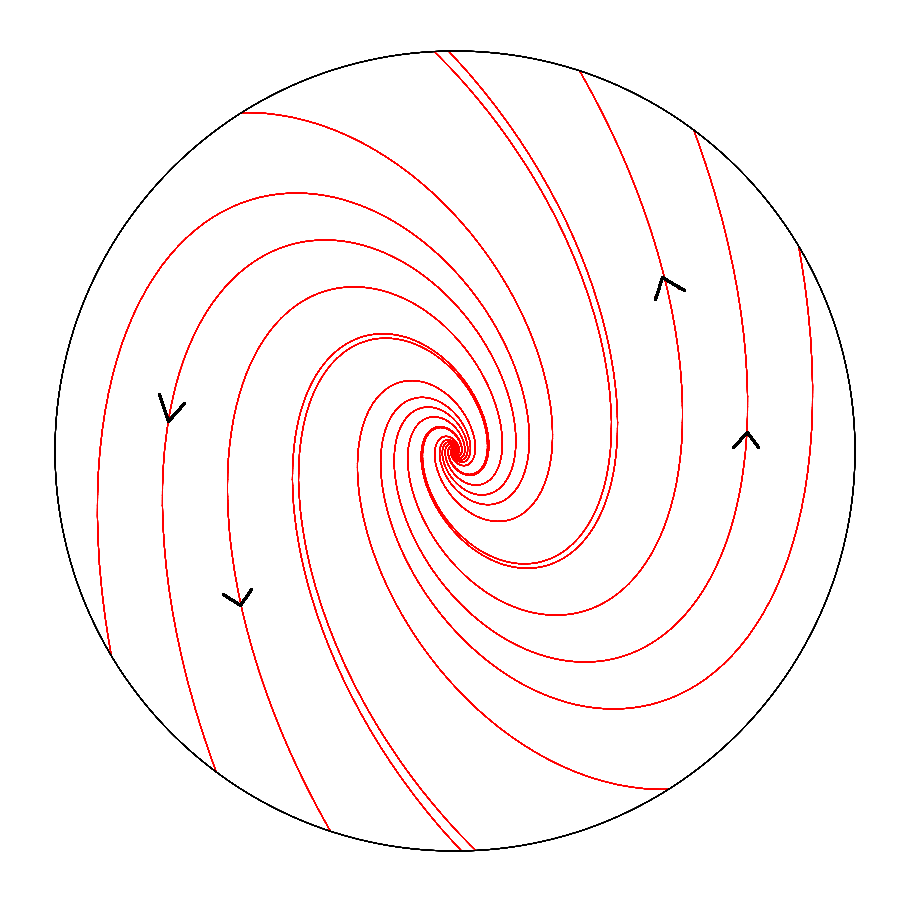
\includegraphics[scale=0.2]{acu_focus_a.png} \]
    \item System E has a continuous conserved quantity that is not
     just a constant, and the equilibrium point at the origin is stable.
    \item System F has a strong Lyapunov function, and one of the
     eigenvalues is $-3$.
   \end{itemize}
  \item[(ii)] Give examples as follows.  The numbers in every matrix
   should be real numbers. \mrks{8}
   \begin{itemize}
    \item[(a)] Give an example of a linear system with an
     anticlockwise centre at the origin.
    \item[(b)] Give an example of a matrix $B$ where
     $\tau=3$ and $\dl=0$.
    \item[(c)] Give an example of a matrix $C$ where the eigenvalues
     are $1+i$ and $1-i$.
    \item[(d)] Give an example of a linear system for which the
     function $U=xy$ is a conserved quantity.
%    \item[(e)] Give an example of a linear system with solution
%     $(x,y)=(e^t,te^t)$. 
   \end{itemize}
 \end{itemize}
\end{problem} 
\begin{solution}\leavevmode
 \begin{itemize}
  \item[(i)]
   \begin{itemize}
    \item[(A)] Here $\tau,\dl>0$ and $\tau^2-4\Dl=60>0$ so we have an
     unstable node. \mks{2}
    \item[(B)] Here we must have eigenvalues $-3\pm 4i$, giving a
     stable focus. \mks{2}
    \item[(C)] Here there is one negative eigenvalue and one positive
     eigenvalue so we have a saddle. \mks{2}
    \item[(D)] The picture shows an anticlockwise unstable focus. \mks{2}
    \item[(E)] As there is a nontrivial conserved quantity, we can
     only have a saddle or a centre.  As saddles are unstable, we must
     have a centre.  \mks{2}
    \item[(F)] As there is a strong Lyapunov function, the origin must
     be asymptotically stable, so it is a stable node or a stable
     focus.  For a stable focus, neither eigenvalues is real.  As one
     of the eigenvalues is $-3$, we must have a stable node.  \mks{2}
   \end{itemize}
  \item[(ii)] 
   \begin{itemize}
    \item[(a)] We need $\dot{x}=ax+by$ and $\dot{y}=cx+dy$ with
     $\tau=a+d=0$ and $\dl=ad-bc>0$ and $c>0$.  The simplest way to do
     this is with $a=d=0$ and $b=-1$ and $c=1$, giving $\dot{x}=-y$
     and $\dot{y}=x$.  \mks{2}
    \item[(b)] We need $B=\bbm a&b\\c&d\ebm$ with $a+d=3$ and
     $ad-bc=0$.  The simplest way to do this is with $a=3$ and
     $b=c=d=0$ giving $B=\bbm 3&0\\ 0&0\ebm$.  Another possibility is
     $B=\bbm 1&2\\1&2\ebm$.  \mks{2}
    \item[(c)] We need
     \begin{align*}
      \tau &= \lm_1+\lm_2 = (1-i) + (1+i) = 2 \\
      \dl &= \lm_1\lm_2 = (1-i)(1+i) = 1 - i^2 = 2.
     \end{align*}
     The simplest way to do this is with $D=\bbm 1&1\\-1&1\ebm$.  \mks{2}
    \item[(d)] The simplest way to do this is with $\dot{x}=x$ and
     $\dot{y}=-y$.  (This gives $\dot{U}=\dot{x}y+x\dot{y}=xy-xy=0$.
     Alternatively, the solutions have the form
     $(x,y)=(x_0e^t,y_0e^{-t})$, giving $U=x_0y_0$ for all $t$.)
     \mks{2}
%    \item[(e)] These functions satisfy $\dot{x}=x$ and $\dot{y}=x+y$. 
%     (This is easy to see, because $\dot{x}=e^t=x$ and
%     $\dot{y}=e^t+te^t=x+y$.)
  \end{itemize}
 \end{itemize}
\end{solution}

\begin{problem} % 2017-18Q1
 \begin{itemize}
  \item[(i)]
   Suppose we have four planar linear systems with
   properties described below.  In each case, find the type of
   equilibrium at the origin. \mrks{12}
   \begin{itemize}
    \item System A has a solution $(x,y)=(\cosh(t),\sinh(t))$.
    \item The matrix for system B has characteristic polynomial
     $t^2-100 t+1000$.
    \item System C has eigenvalues $10+\pi i$ and $10-\pi i$.
    \item System D has a continuous conserved quantity that is not
     just a constant, and the equilibrium point at the origin is stable.
    \item System E has the following phase diagram:
     \[ 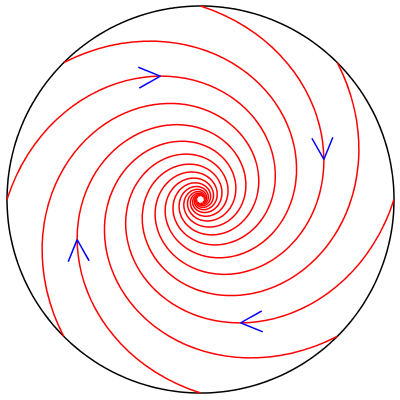
\includegraphics[scale=0.4]{cws_focus_a.png} \]
    \item System F corresponds to the following point in the $(\tau,\dl)$-plane.
     \begin{center}
      \begin{tikzpicture}[scale=2.5]
       \draw (-1.2,-0.3) rectangle (1.2,1.2);
       \draw[thick,cyan] (-1,0) -- (0,0);
       \draw[thick,orange,->] (0,0) -- (1,0);
       \draw[thick,olivegreen,->] (0,0) -- (0,1);
       \draw[thick,blue,smooth] (-1,1) -- (-0.9,0.81) -- (-0.8,0.64) --
         (-0.7,0.49) -- (-0.6,0.36) -- (-0.5,0.25) -- (-0.4,0.16) --
         (-0.3,0.09) -- (-0.2,0.04) -- (-0.1,0.01) -- (0,0);
       \draw[thick,red,smooth] (1,1) -- (0.9,0.81) -- (0.8,0.64) --
         (0.7,0.49) -- (0.6,0.36) -- (0.5,0.25) -- (0.4,0.16) --
         (0.3,0.09) -- (0.2,0.04) -- (0.1,0.01) -- (0,0);
       \draw(0,1) node[anchor=south]{$\ss\dl$};
       \draw(1,0) node[anchor=west]{$\ss\tau$};
       \fill[black] (-0.8,0.1) circle(0.02);
      \end{tikzpicture}
     \end{center}
   \end{itemize}
  \item[(ii)] Give examples as follows.  The numbers in every matrix
   should be real numbers. \mrks{8}
   \begin{itemize}
    \item[(a)] Give an example of a linear system with an
     clockwise stable focus at the origin.
    \item[(b)] Give an example of a matrix $B$ where
     $\tau=7$ and $\dl=10$.
    \item[(c)] Give an example of a matrix $C$ where one eigenvalue
     is $10i$.
    \item[(d)] Give an example of a linear system for which the
     function $U=x^2+y^2$ is a conserved quantity.
   \end{itemize}
 \end{itemize}
\end{problem} 
\begin{solution}\leavevmode
 \begin{itemize}
  \item[(i)]
   \begin{itemize}
    \item[(A)] Here the exponentials involved in the colution
     \[ (x,y) = (\cosh(t),\sinh(t)) = (e^t+e^{-t},e^t-e^{-t})/2 \]
     are $e^t$ and $e^{-t}$, so the eigenvalues are $+1$ and $-1$.  As
     there is one positive eigenvalue and one negative eigenvalue, we
     have a saddle. \mks{2}
    \item[(B)] Here $\tau=100>0$ and $\dl=1000>0$ and
     $\tau^2-4\dl=6000>0$ so we have an unstable node. \mks{2}
    \item[(C)] Here we have two complex eigenvalues with positive real
     part so we have an unstable focus. \mks{2}
    \item[(D)] As there is a nontrivial conserved quantity, we can
     only have a saddle or a centre.  As saddles are unstable, we must
     have a centre.  \mks{2}
    \item[(E)] The picture shows an clockwise stable focus. \mks{2}
    \item[(F)] The marked point is in the region where $\tau<0$ and
     $\dl > 0$ and $\tau^2-4\dl > 0$ so we have a stable node.  \mks{2}
   \end{itemize}
  \item[(ii)] 
   \begin{itemize}
    \item[(a)] We need $\dot{x}=ax+by$ and $\dot{y}=cx+dy$ with
     $\tau=a+d<0$ and $\dl=ad-bc>0$ and $\tau^2-4\dl < 0$ and $c<0$.
     The simplest way to do this is with $a=c=d=-1$ and $b=1$, giving
     the matrix $A=\bbm -1 & 1 \\ -1 & -1\ebm$.  \mks{2}
    \item[(b)] We need $B=\bbm a&b\\c&d\ebm$ with $a+d=7$ and
     $ad-bc=10$.  The simplest answer is $B=\bbm 2&0\\0&5\ebm$.  There
     are also many other possibiities, such as 
     $B=\bbm 3&2\\1&4\ebm$.  \mks{2}
    \item[(c)] If one eigenvalue is $\lm_1=10i$ then the other one must be
     $\lm_2=-10i$, giving $\tau=\lm_1+\lm_2=0$ and
     $\dl=\lm_1\lm_2=100$.  The simplest matrix like this is
     $C=\bsm 0&10\\-10&0\esm$. \mks{2}
    \item[(d)] The simplest way to do this is with $\dot{x}=y$ and
     $\dot{y}=-x$.  (This gives $\dot{U}=2\dot{x}x+2\dot{y}y=2(yx-xy)=0$.)
     \mks{2}
  \end{itemize}
 \end{itemize}
\end{solution}

%%%%%%%%%%%%%%%%%%%%%%%%%%%%%%%%%%%%%%%%%%%%%%%%%%%%%%%%%%%%%%%%%%%%%% 
%%%%%%%%%%%%%%%%%%%%%%%%%%%%%%%%%%%%%%%%%%%%%%%%%%%%%%%%%%%%%%%%%%%%%%
%%%%%%%%%%%%%%%%%%%%%%%%%%%%%%%%%%%%%%%%%%%%%%%%%%%%%%%%%%%%%%%%%%%%%%
%%%%%%%%%%%%%%%%%%%%%%%%%%%%%%%%%%%%%%%%%%%%%%%%%%%%%%%%%%%%%%%%%%%%%%

\np

\section*{Question 2}

\begin{problem} % 2013-14 Q2
 \begin{itemize}
  \item[(i)]
   Consider the system where 
   \begin{align*}
    \dot{x} &= x^2+2xy+y^2-1 \\
    \dot{y} &= x^2-2xy+y^2-1.
   \end{align*}

   \begin{itemize}
    \item[(a)] Draw a diagram showing the $x$-nullcline, the
     $y$-nullcline and the region where $\dot{x}<0<\dot{y}$. \mrks{6}
    \item[(b)] Find and classify the equilibrium points. \mrks{6}
   \end{itemize}
  \item[(ii)]
   Consider the system where 
   \begin{align*}
    \dot{x} &= -2(1+x^2+y^2)y \\
    \dot{y} &= 3(1+x^2+y^2)x.
   \end{align*}
   \begin{itemize}
    \item[(a)] Find $p$ and $q$ such that the function $U=px^2+qy^2$
     is a conserved quantity.  \mrks{3}
    \item[(b)] Consider the flow line that has $(x,y)=(1,6)$ at
     $t=0$.  Where does this cross the $x$-axis? \mrks{4}
    \item[(c)] Explain carefully why the origin is a stable
     equilibrium point, but is not asymptotically stable. \mrks{3}
    \item[(d)] Show that there are no other equilibrium points. \mrks{3}
   \end{itemize}
 \end{itemize}
\end{problem}
\begin{solution}
 \textbf{Most of this is similar to questions in the lectures and on the
  problem sheets.  However, (ii)(b) which is unseen, and the students
  have rarely been asked for ``careful explanation'' as in (ii)(c).}
 \begin{itemize}
  \item[(i)]
   \begin{itemize}
    \item[(a)] The $x$-nullcline is given by $x^2+2xy+y^2=1$, or
     equivalently $(x+y)^2=1$, so $x+y=\pm 1$.  Thus, it is the union of
     two straight lines, one with equation $y=1-x$ and the other with
     equation $y=-1-x$ \mks{2}.  Similarly, the $y$-nullcline is given by
     $x^2-2xy+y^2=1$, or $x-y=\pm 1$.  This is the union of the lines
     $y=x+1$ and $y=x-1$ \mks{2}.  For $\dot{x}<0<\dot{y}$ we must have
     $(x+y)^2<1<(x-y)^2$, so $-1<x+y<1$ but $x-y$ is either less than
     $-1$ or greater than $+1$.  The relevant region is shaded in the
     diagram below. \mks{2}
     \begin{center}
      \begin{tikzpicture}[scale=1.5]
       \fill[cyan!30] (-2,2) -- (-1,2) -- (0,1) -- (-1,0) -- (-2,1) -- cycle;
       \fill[cyan!30] (2,-2) -- (1,-2) -- (0,-1) -- (1,0) -- (2,-1) -- cycle;
       \draw[thick,blue ] (-1, 2) -- ( 2,-1);
       \draw[thick,blue ] (-2, 1) -- ( 1,-2);
       \draw[thick,green] (-2,-1) -- ( 1, 2);
       \draw[thick,green] (-1,-2) -- ( 2, 1);
       \draw (-1, 1) node {$\ss\dot{x}<0<\dot{y}$};
       \draw ( 1,-1) node {$\ss\dot{x}<0<\dot{y}$};
       \draw ( 2,-1) node[anchor=west ] {$\ss y=1-x$};
       \draw ( 2, 1) node[anchor=west ] {$\ss y=x-1$};
       \draw (-2,-1) node[anchor=east ] {$\ss y=x+1$};
       \draw ( 1,-2) node[anchor=north] {$\ss y=-1-x$};
      \end{tikzpicture}
     \end{center}
    \item[(b)] From part~(i) it is clear that the equilibrium points are
     as follows:
     \[ a_1 = ( 0, 1) \qquad
        a_2 = ( 0,-1) \qquad
        a_3 = ( 1, 0) \qquad
        a_4 = (-1, 0). \mks{2}
     \]
     The Jacobian is
     \[ J = \bbm \partial f/\partial x & 
                 \partial f/\partial y \\
                 \partial g/\partial x & 
                 \partial g/\partial y \ebm
          = \bbm 2(x+y) & 2(x+y) \\
                 2(x-y) & 2(y-x) \ebm.  \mks{2}
     \]
     Using this, the equilibrium points can be classified as follows:
     \[ \renewcommand{\arraystretch}{1.5}
        \begin{array}{|c|c|c|c|c|c|c|c|} \hline
             &  x &  y & J                      & \tau & \dl & \tau^2-4\dl & \text{ type } \\ \hline
         a_1 &  0 &  1 & \bsm  2& 2\\-2& 2 \esm &  4   &  8  & -16         & \text{ unstable focus } \\ \hline
         a_2 &  0 & -1 & \bsm -2&-2\\ 2&-2 \esm & -4   &  8  & -16         & \text{   stable focus } \\ \hline
         a_3 &  1 &  0 & \bsm  2& 2\\ 2&-2 \esm &  0   & -8  &  32         & \text{ saddle }         \\ \hline
         a_4 & -1 &  0 & \bsm -2&-2\\-2& 2 \esm &  0   & -8  &  32         & \text{ saddle }         \\ \hline
        \end{array} \mks{2}
     \]
   \end{itemize}
  \item[(ii)]
   \begin{itemize}
    \item[(a)] If $U=px^2+qy^2$, then 
     \begin{align*}
      \dot{U} &= U_x\dot{x} + U_y\dot{y} \mk
               = (2px)(-2(1+x^2+y^2)y) + (2qy)(3(1+x^2+y^2)x) \\
       &= 2xy(1+x^2+y^2)(-2p+3q). \mk
     \end{align*}
     We now take $p=3$ and $q=2$, so $U=3x^2+2y^2$.  With these values
     we have $-2p+3q=0$ so $\dot{U}=0$, so $U$ is a conserved
     quantity. \mk
    \item[(b)] Suppose that when $t=0$ we have $(x,y)=(1,6)$, so
     $U=3\tm 1^2+2\tm 6^2=75$ \mk.  As $U$ is conserved, we have
     $3x^2+2y^2=75$ for all $t$ \mk.  In particular, when the flow line
     crosses the $x$-axis we have $y=0$ and so $3x^3=75$, which gives
     $x=\pm 5$. \mk Thus, the flow line crosses the $x$-axis at $(-5,0)$
     and $(5,0)$ \mk.
    \item[(c)] It is clear that the function $U=3x^2+2y^2$ is positive
     definite \mk.  Moreover, the derivative $\dot{U}=0$ is negative
     semidefinite, so $U$ is a weak Lyapunov function, which means
     that the origin is a stable equilibrium \mk.  However, as $U$ is
     conserved, any flow line that starts away from the origin cannot
     converge to the origin.  This means that the origin is not
     asymptotically stable \mk.
    \item[(d)] At any equilibrium point we must have
     $\dot{x}=-2(1+x^2+y^2)y=0$ and $\dot{y}=3(1+x^2+y^2)x=0$ \mk.  As
     $1+x^2+y^2$ is always strictly positive, we can divide by it \mk,
     giving $-2y=0$ and $3x=0$, so $(x,y)=(0,0)$.  Thus, the origin is
     the only equilibrium point \mk.
   \end{itemize}
 \end{itemize}
\end{solution}

\begin{problem} % 2013-14 R Q2
 \begin{itemize}
  \item[(i)]
   Consider the system where 
   \begin{align*}
    \dot{x} &= x^2+y^2-1 \\
    \dot{y} &= x.
   \end{align*}

   \begin{itemize}
    \item[(a)] Draw a diagram showing the $x$-nullcline, the
     $y$-nullcline and the region where $\dot{x},\dot{y}<0$. \mrks{4}
    \item[(b)] Find and classify the equilibrium points. \mrks{5}
    \item[(c)] Show that the function $U=e^{-2y}(x^2+y^2+y-\half)$ is
     a conserved quantity. \mrks{4}
   \end{itemize}
  \item[(ii)]
   Consider the system where 
   \begin{align*}
    \dot{x} &= -\sin(x)\cos(y) \\
    \dot{y} &= -\cos(x)\sin(y),
   \end{align*}
   and the functions $V=1-\cos(x)\cos(y)$ and $W=2-V=1+\cos(x)\cos(y)$.
   \begin{itemize}
    \item[(a)] Show that $V\geq 0$ and $\dot{V}\leq 0$.  \mrks{4}
    \item[(b)] Find the equilibrium points, and the values of $V$ at the
     equilibrium points.  You should find that some equilibrium points
     have $V=0$, some have $V=1$ and some have $V=2$. \mrks{7}
    \item[(c)] Use Lyapunov theory to show that the origin is an
     asymptotically stable equilibrium point. \mrks{6}
%    \item[(d)] Use the function $W$ to show that the point $(\pi,\pi)$
%     is an unstable equilibrium. \mrks{5}
   \end{itemize}
 \end{itemize}
\end{problem}
\begin{solution}
 \begin{itemize}
  \item[(i)]
   \begin{itemize}
    \item[(a)] The $x$-nullcline is given by $x^2+y^2=1$, which
     describes the unit circle.  Inside the circle we have
     $\dot{x}<0$, and outside the circle we have $\dot{x}>0$ \mk.  The
     $y$-nullcline is given by $x=0$.  In the left half plane we have
     $\dot{y}<0$, and in the right half plane we have $\dot{y}>0$ \mk.  
     The required diagram is as follows \mks{2}:
     \begin{center}
      \begin{tikzpicture}[scale=2]
       \fill[cyan!30] (0,0) circle(1);
       \fill[white] (0,-1) rectangle (1,1); 
       \draw[thick,blue ] (0,0) circle(1);
       \draw[thick,green] (0,-1.5) -- (0,1.5);
       \draw (-1.5, 0.1) node {$\ss\dot{x}>0$};
       \draw (-1.5,-0.1) node {$\ss\dot{y}<0$};
       \draw (-0.5, 0.1) node {$\ss\dot{x}<0$};
       \draw (-0.5,-0.1) node {$\ss\dot{y}<0$};
       \draw ( 0.5, 0.1) node {$\ss\dot{x}<0$};
       \draw ( 0.5,-0.1) node {$\ss\dot{y}>0$};
       \draw ( 1.5, 0.1) node {$\ss\dot{x}>0$};
       \draw ( 1.5,-0.1) node {$\ss\dot{y}>0$};
       \draw (0.7,0.7) node[anchor=south west] {$\ss x^2+y^2=1$};
       \draw (0.0,1.3) node[anchor=west] {$\ss x=0$};
      \end{tikzpicture}
     \end{center}
    \item[(b)] From part~(i) it is clear that the equilibrium points are
     as follows:
     \[ a_1 = ( 0, 1) \qquad
        a_2 = ( 0,-1) . \mk
     \]
     The Jacobian is
     \[ J = \bbm \partial f/\partial x & 
                 \partial f/\partial y \\
                 \partial g/\partial x & 
                 \partial g/\partial y \ebm
          = \bbm 2x & 2y \\
                 1 & 0 \ebm.  \mk
     \]
     Using this, the equilibrium points can be classified as follows:
     \[ \renewcommand{\arraystretch}{1.5}
        \begin{array}{|c|c|c|c|c|c|c|c|} \hline
             &  x &  y & J                      & \tau & \dl & \tau^2-4\dl & \text{ type } \\ \hline
         a_1 &  0 &  1 & \bsm  0& 2\\ 1& 0 \esm &  0   & -2  &  8          & \text{ saddle\mk } \\ \hline
         a_2 &  0 & -1 & \bsm  0&-2\\ 1& 0 \esm &  0   &  2  & -8          & \text{ anticlockwise centre\mks{2} } \\ \hline
        \end{array}
     \]
    \item[(c)] If $U=e^{-2y}(x^2+y^2+y-\half)$ then
     \begin{align*}
      U_x &= e^{-2y}\tm 2x \mk \\
      U_y &= -2e^{-2y}(x^2+y^2+y-\half) + e^{-2y}(2y+1) \\
          &= e^{-2y}(-2x^2-2y^2+2) \mk \\
      \dot{U} &= (x^2+y^2-1)U_x + xU_y \\
          &= e^{-2y}(2x^3+2xy^2-2x-2x^3-2xy^2+2x) = 0. \mks{2}
     \end{align*}
     Thus, $U$ is a conserved quantity.
   \end{itemize}
  \item[(ii)]
   \begin{itemize}
    \item[(a)] First, $\cos(x)$ and $\cos(y)$ both lie in the interval
     $[-1,1]$, so $\cos(x)\cos(y)$ also lies in $[-1,1]$, so the number
     $V=1-\cos(x)\cos(y)$ lies in $[0,2]$; in particular, $V\geq 0$. \mks{2}
     Next, we have 
     \begin{align*}
      V_x &= \sin(x)\cos(y) \\
      V_y &= \cos(x)\sin(y) \\
      \dot{V} &= V_x\tm(-\sin(x)\cos(y)) + V_y\tm(-\cos(x)\sin(y)) \\
       &= -(\sin^2(x)\cos^2(y)+\cos^2(x)\sin^2(y)) \leq 0. \mks{2}
     \end{align*}
    \item[(b)] At an equilibrium point we must have
     $\dot{x}=-\sin(x)\cos(y)=0$, so $\sin(x)=0$ or $\cos(y)=0$.  
     Similarly, we must have $\dot{y}=-\cos(x)\sin(y)=0$, so
     $\cos(x)=0$ or $\sin(y)=0$.  \mk This seems to give four
     possibilities:
     \begin{itemize}
      \item[(1)] $\sin(x)=0$ and $\cos(x)=0$
      \item[(2)] $\sin(x)=0$ and $\sin(y)=0$
      \item[(3)] $\cos(y)=0$ and $\cos(x)=0$
      \item[(4)] $\cos(y)=0$ and $\sin(y)=0$.
     \end{itemize}
     However, $\sin^2(x)+\cos^2(x)$ is always equal to one, so
     $\sin(x)$ and $\cos(x)$ cannot both be zero, so case~(1) is
     impossible.  Similarly, case~(4) is impossible \mk. In case~(2) we
     have $x=n\pi$ and $y=m\pi$ for some integers $n$ and $m$ \mk.  This
     gives $\cos(x)=(-1)^n$ and $\cos(y)=(-1)^m$ so $V=1-(-1)^{n+m}$ \mk.
     Thus, if $n+m$ is even then $V=0$, and if $n+m$ is odd then
     $V=2$ \mk.  In case~(3) we have $x=(n+\half)\pi$ and $y=(m+\half)\pi$
     for some integers $n$ and $m$ \mk, and $V=1-\cos(x)\cos(y)=1$ \mk.
    \item[(c)] We saw in~(a) that $V$ is positive semidefinite and
     $\dot{V}$ is negative semidefinite everywhere in the whole
     plane.  Now consider the region 
     \[ R = \{(x,y)\st -\pi/2 < x,y < \pi/2\}.  \]
     In this region we have $0<\cos(x),\cos(y)\leq 1$, so the only way
     that the function $V=1-\cos(x)\cos(y)$ can be zero is if
     $\cos(x)=\cos(y)=1$ which means that $x=y=0$.  Thus, $V$ is
     positive definite on $R$ \mks{3}.  We also saw that 
     \[ \dot{V} = -(\sin^2(x)\cos^2(y)+\cos^2(x)\sin^2(y)). \]
     This can only be zero if $\sin(x)\cos(y)=0$ and also
     $\cos(x)\sin(y)=0$ \mk.  On $R$ we have $\cos(x)>0$ and $\cos(y)>0$,
     so we can only have $\dot{V}=0$ if $\sin(x)=\sin(y)=0$, which
     means that $x=y=0$ \mk.  Thus, $\dot{V}$ is negative definite on $R$,
     so $V$ is a strong Lyapunov function on $R$, so the origin is
     asymptotically stable \mk.  
%    \item[(d)] Recall that $W=2-V$.  As $V$ lies between $0$ and $2$
%     we see that $W$ is positive semidefinite \mk.  As $\dot{V}\leq 0$ we
%     see that $\dot{W}\geq 0$, so $\dot{W}$ is positive semidefinite \mk.  
%     On the region 
%     \[ R' = \{(x,y)\st \pi/2 < x,y < 3\pi/2\} \]
%     we find (as in~(c)) that both $W$ and $\dot{W}$ are strictly
%     positive, except at the point $(\pi,\pi)$ \mks{2}.  Thus, the standard
%     Lyapunov instability criterion shows that $(\pi,\pi)$ is an
%     unstable equilibrium \mk.
   \end{itemize}
 \end{itemize}
\end{solution}

\begin{problem} % 2014-15 Q2
 \begin{itemize}
  \item[(i)]
   Consider the system where 
   \begin{align*}
    \dot{x} &= 5y + 12 - 12 x^2 \\
    \dot{y} &= 2y - 12 + 12 x^2.
   \end{align*}

   \begin{itemize}
    \item[(a)] Draw a diagram showing the $x$-nullcline and the
     $y$-nullcline.  For each region in the diagram, say whether
     $\dot{x}>0$ or $\dot{x}<0$, and whether $\dot{y}>0$ or
     $\dot{y}<0$. \mrks{5}
    \item[(b)] Find the equilibrium points. \mrks{2}
    \item[(c)] For each equilibrium point, find the eigenvalues
     of the relevant matrix, and thus classify the point. \mrks{4}
   \end{itemize}
  \item[(ii)]
   Consider the function $V=x^4+x^2y^2+y^4$, and the system where 
   \begin{align*}
    \dot{x} &= f(x,y) = 2y^3+x^2y-x \\
    \dot{y} &= g(x,y) = -2x^3-xy^2-y.
   \end{align*}
   Note that the origin is an equilibrium point.
   \begin{itemize}
    \item[(a)] Show that $\dot{V}=-4V$.  \mrks{4}
%    \item[(d)] Deduce that the origin is the only equilibrium point.
    \item[(b)] What can you prove about the stability of $(0,0)$
     for the linearisation of the above system?  What can you deduce
     about the stability of the original system? \mrks{6}
    \item[(c)] What can you prove about the stability of $(0,0)$
     using Lyapunov theory? \mrks{4}
   \end{itemize}
 \end{itemize}
\end{problem}
\begin{solution}
 \begin{itemize}
  \item[(i)] \textbf{This is a standard problem.}\\
   \begin{itemize}
    \item[(a)] The $x$-nullcline is given by $y=\frac{12}{5}(x^2-1)$ \mk,
     and the $y$-nullcline is given by $y=6(1-x^2)$ \mk.  Note also that
     $\dot{x}$ is an increasing function of $y$, so $\dot{x}>0$ above
     the $x$-nullcline, and $\dot{x}<0$ below the $x$-nullcline.
     Similarly, $\dot{y}>0$ above the $y$-nullcline, and $\dot{y}<0$
     below the $y$-nullcline.  This gives the following picture:
     \begin{center}
      \begin{tikzpicture}[scale=1.2]
       \clip (-4,-4) -- (4,-4) -- (4,4) -- (-4,4) -- cycle;
       \draw[blue,domain=-2:2,smooth,variable=\x]
        plot({\x},{0.5*2.4*(\x*\x - 1)});
       \draw[green,domain=-2:2,smooth,variable=\x]
        plot({\x},{0.5*(-6)*(\x*\x - 1)});
       \fill[black] (-1,0) circle(0.05);
       \fill[black] ( 1,0) circle(0.05);
       \draw (-2, 0.0) node {$\scriptstyle \dot{x}<0,\;\dot{y}>0$};
       \draw ( 0, 0.0) node {$\scriptstyle \dot{x}>0,\;\dot{y}<0$};
       \draw ( 2, 0.0) node {$\scriptstyle \dot{x}<0,\;\dot{y}>0$};
       \draw ( 0, 3.5) node {$\scriptstyle \dot{x}>0,\;\dot{y}>0$};
       \draw ( 0,-2.5) node {$\scriptstyle \dot{x}<0,\;\dot{y}<0$};
      \end{tikzpicture}
      \mks{3}
     \end{center}
    \item[(b)] The equilibrium points are given by
     $y=\frac{12}{5}(x^2-1)=6(1-x^2)$, which gives $y=x^2-1=0$, so
     $y=0$ and $x=\pm 1$.  Thus, the only equilibrium points are
     $a_1=(1,0)$ and $a_2=(-1,0)$ \mks{2}. 
    \item[(c)] The Jacobian is
     \[ J = \bbm \partial f/\partial x & 
                 \partial f/\partial y \\
                 \partial g/\partial x & 
                 \partial g/\partial y \ebm
          = \bbm -24x & 5 \\
                 24x & 2 \ebm,
     \]
     which has trace $\tau=2-24x$ and determinant $\dl=-24\tm 7x$.

     At $a_1$ we have $J=\bbm -24&5\\ 24&2\ebm$, which has $\tau=-22$
     and $\dl=-168$ and $\tau^2-4\dl=1156=34^2$.  The eigenvalues are
     $(-22\pm 34)/2$, which gives $\lm_1=-28$ and $\lm_2=6$
     \mk. As one eigenvalue is negative and the other is positive,
     we have a saddle \mk.  
%     The eigenvector $u_1$ must be annihilated by $J-\lm_1I=\bbm
%     4&5\\24&30\ebm$, so we can take $u_1=\bbm 5\\ -4\ebm$ \mks{2}.
%     The eigenvector $u_2$ must be annihilated by $J-\lm_2I=\bbm -30&5
%     \\ 24&-4\ebm$, so we can take $u_2=\bbm 1\\6\ebm$ \mks{2}.

     At $a_2$ we have $J=\bbm 24&5\\-24&2\ebm$, which has $\tau=26$
     and $\dl=168$ and $\tau^2-4\dl=4=2^2$.  The eigenvalues are
     $(26\pm 2)/2$, which gives $\lm_1=12$ and $\lm_2=14$ \mk.
     As both eigenvalues are positive (and different) we have an
     unstable node \mk. 
%     The eigenvector $u_1$ must be annihilated by $J-\lm_1I=\bbm
%     12&5\\-24&-10\ebm$, so we can take $u_1=\bbm 5\\ -12\ebm$
%     \mks{2}.  The eigenvector $u_2$ must be annihilated by
%     $J-\lm_2I=\bbm 10&5 \\-24&-12\ebm$, so we can take $u_2=\bbm
%     1\\-2\ebm$ \mks{2}.
   \end{itemize}
  \item[(ii)] \textbf{This is a standard problem.}\\
   \begin{itemize}
    \item[(a)] $V_x=4x^3+2xy^2$ and $V_y=2x^2y+4y^3$ \mks{2} so 
     \begin{align*}
      \dot{V} &= V_x\dot{x} + V_y\dot{y} \mk \\
       &= (4x^3+2xy^2)(2y^3+x^2y-x) + (2x^2y+4y^3)(-2x^3-xy^2-y) \\
       &= 8x^3y^3+4x^5y-4x^4+4xy^5+2x^3y^3-2x^2y^2 \\
       &\quad - 4x^5y-2x^3y^3-2x^2y^2-8x^3y^3-4xy^5-4y^4 \\
       &= -4x^4-4x^2y^2-4y^4 = -4V. \mk
     \end{align*}
%    \item[(d)] If $x=y=0$ then $\dot{x}=f(0,0)=0$ and
%     $\dot{y}=g(0,0)=0$; so $(0,0)$ is an equilibrium point. \mk
%     Conversely, if $\dot{x}=\dot{y}=0$ at some point, then the
%     quantity $\dot{V}=V_x\dot{x}+V_y\dot{y}$ will also be zero at
%     that point.  However, $\dot{V}=-4V$, so the quantity
%     $V=x^4+x^2y^2+y^4$ will also be zero.  As $x^4$, $x^2y^2$ and
%     $y^4$ are all nonnegative, we can only have $V=0$ if
%     $x^4=x^2y^2=y^4=0$, which means that $x=y=0$.  Thus, $(0,0)$ is
%     the \emph{only} equilibrium point. \mks{3}
    \item[(b)] The Jacobian is 
     \[ J = \bbm \partial f/\partial x & 
                 \partial f/\partial y \\
                 \partial g/\partial x & 
                 \partial g/\partial y \ebm
          = \bbm 2xy-1 & x^2+6y^2 \\
                 -6x^2-y^2 & -2xy-1 \ebm, \mk
     \]
     and this becomes $J=-I$ at the origin \mk.  The linearisation
     therefore has an asymptotically stable node at the origin \mk.  The
     eigenvalues are both equal to $-1$, so the real part is nonzero,
     so the Hartman-Grobman theorem is applicable.  We can thus deduce
     that the original system also has an asymptotically stable
     equilibrium at the origin \mks{3}.
    \item[(c)] As $x^4$, $y^4$ and $x^2y^2$ are always nonnegative, it
     is easy to see that $V\geq 0$ everywhere, and that $V$ can only
     be zero at $(0,0)$.  In other words, the function $V$ is positive
     definite \mk.  It follows that the function $\dot{V}=-4V$ is negative
     definite \mk, and thus that $V$ is a strong Lyapunov function \mk.  This
     implies that the origin is an asymptotically stable equilibrium
     point \mk. 
   \end{itemize}
 \end{itemize}
\end{solution}

\begin{problem} % 2014-15 R Q2
 \begin{itemize}
  \item[(i)]
   Consider the system where 
   \begin{align*}
    \dot{x} &= e^{y+x}-e \\
    \dot{y} &= e^{y-x}-e.
   \end{align*}

   \begin{itemize}
    \item[(a)] Draw a diagram showing the $x$-nullcline and the
     $y$-nullcline.  For each region in the diagram, say whether
     $\dot{x}>0$ or $\dot{x}<0$, and whether $\dot{y}>0$ or
     $\dot{y}<0$. \mrks{5}
    \item[(b)] Find and the equilibrium point, find the eigenvalues 
     of the relevant matrix, and thus classify the point. \mrks{6}
    \item[(c)] Explain what we can conclude from this about the
     stability of the original system. \mrks{2}
    \item[(d)] Sketch the flow lines. \mrks{3}
   \end{itemize}
  \item[(ii)]
   Consider the system where 
   \begin{align*}
    \dot{x} &= -x+\sinh(y) \\
    \dot{y} &= -y-\sinh(x),
   \end{align*}
   and the functions $V=\cosh(x)+\cosh(y)-2$.  Analyse the behaviour
   of $V$ and $\dot{V}$, and explain what we can deduce about the
   stability of equilibrium points. \mrks{9}
 \end{itemize}
\end{problem}
\begin{solution}
 \begin{itemize}
  \item[(i)] \textbf{This is a standard type of problem.}
   \begin{itemize}
    \item[(a)] The $x$-nullcline is given by $e^{y+x}=e$, or
     equivalently $y+x=1$ or $y=1-x$ \mk.  When $y>1-x$ we have
     $\dot{x}>0$, and when $y<1-x$ we have $\dot{x}<0$ \mk.  Similarly,
     the $y$-nullcline is given by $e^{y-x}=e$, or equivalently
     $y=1+x$ \mk.  When $y>1-x$ we have $\dot{x}>0$, and when
     $y<1-x$ we have $\dot{x}<0$ \mk.  The required diagram is as
     follows \mk: 
     \begin{center}
      \begin{tikzpicture}[scale=2]
       \draw[thin,gray,->] (-2, 0) -- (2,0); 
       \draw[thin,gray,->] ( 0,-1) -- (0,2); 
       \draw[thick,blue ] (-1,2) -- (2,-1);
       \draw[thick,green] (-2,-1) -- (1,2);
       \fill[black] (0,1) circle(0.03);
       \draw ( 1.9,-0.9) node[anchor=south west] {$\ss\dot{x}>0$};
       \draw ( 1.9,-0.9) node[anchor=north east] {$\ss\dot{x}<0$};
       \draw (-1.9,-0.9) node[anchor=south east] {$\ss\dot{y}>0$};
       \draw (-1.9,-0.9) node[anchor=north west] {$\ss\dot{y}<0$};
      \end{tikzpicture}
     \end{center}
    \item[(b)] For an equilibrium point we need $y=1+x$ and also
     $y=1-x$ which gives $x=0$ and $y=1$.  Thus, $(0,1)$ is the only
     equilibrium point \mk.  The Jacobian is 
     \[ J = \bbm \partial f/\partial x & 
                 \partial f/\partial y \\
                 \partial g/\partial x & 
                 \partial g/\partial y \ebm
          = \bbm e^{y+x} & e^{y+x} \\
                 -e^{y-x} & e^{y-x} \ebm.  \mk
     \]
     At $(0,1)$ this becomes $J=\bbm e&e \\ -e&e\ebm$ \mk.  This has
     $\tau=2e$ and $\dl=2e^2$ so $\tau^2-4\dl=-4e^2$.  This means that
     the eigenvalues are $(2e\pm\sqrt{-4e^2})/2=(1\pm i)e$ \mk.  These are
     complex, with positive real part, so the linearisation has an
     unstable focus \mk.  As the bottom left entry in $J$ is negative, the
     rotation is clockwise \mk.
    \item[(c)] As the eigenvalues have nonzero real part, the
     Hartman-Grobman theorem is applicable \mk, and we conclude that
     $(0,1)$ is also an unstable equilibrium point for the 
     original system. \mk
    \item[(d)] The picture is as follows.
     \[ 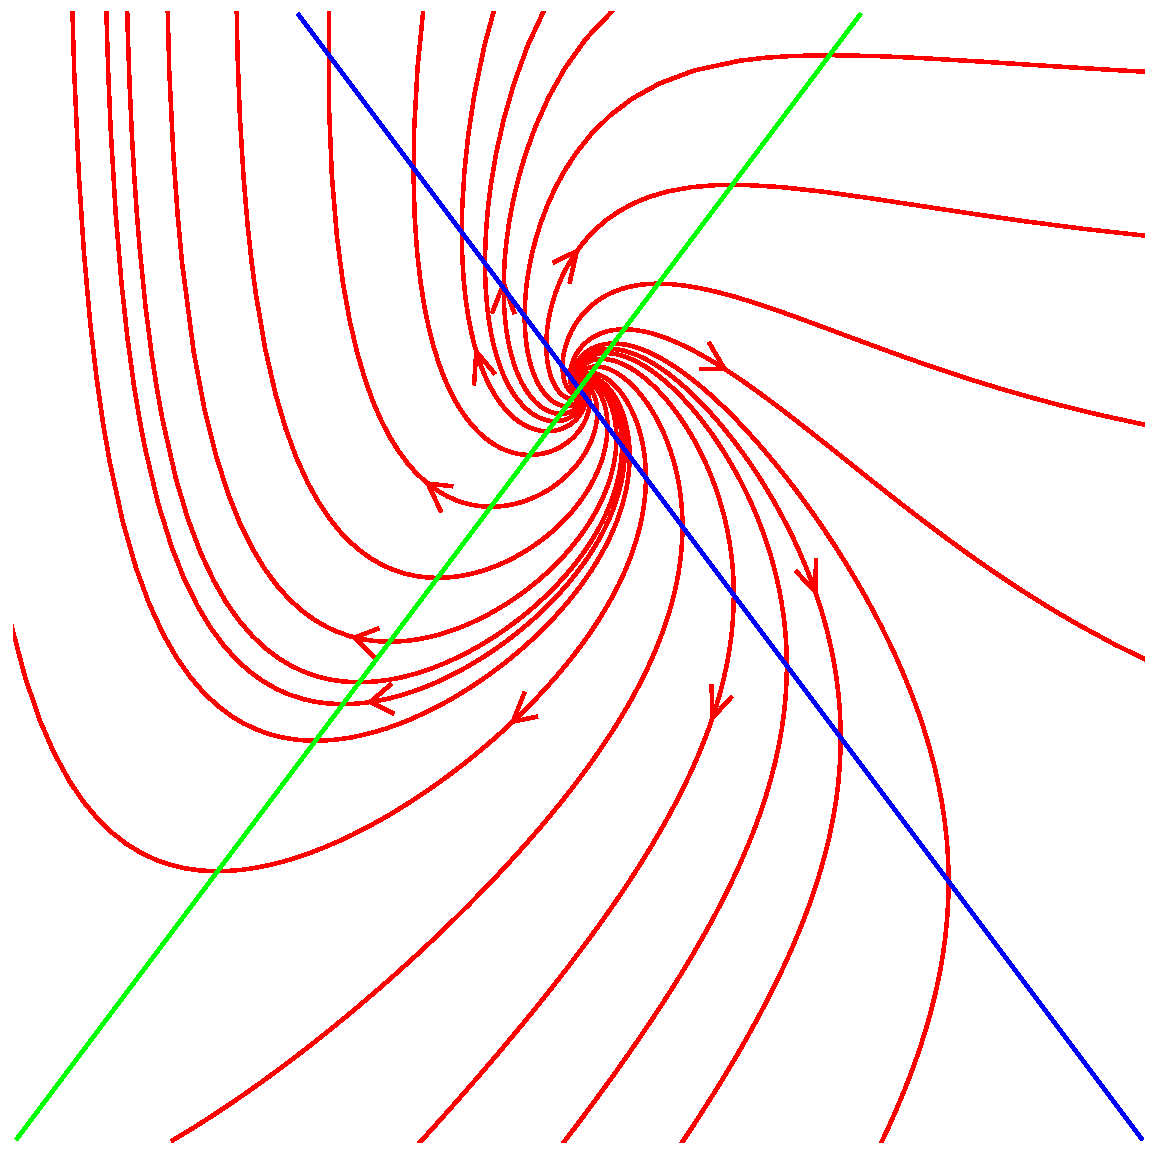
\includegraphics[scale=0.4]{expexp.pdf} \]
     Note that the flow lines cross the $x$-nullcline vertically and
     the $y$-nullcline horizontally, in the direction indicated by the
     previous diagram.  Note also that the flow lines spiral outwards
     clockwise from the equilibrium point. \mks{3}
   \end{itemize}
  \item[(ii)] \textbf{This is a standard type of problem, but the 
    students have not seen many examples with hyperbolic functions.
   }
   We have $\cosh(x)=(e^x+e^{-x})/2\geq 1$ for all $x$,
   with equality if and only if $x=0$.  Similarly $\cosh(y)\geq 1$,
   with equality if and only if $y=0$ \mk.  We can thus consider $V$ as
   the sum of the nonnegative functions $\cosh(x)-1$ and $\cosh(y)-1$,
   and we conclude that $V\geq 0$, we equality if and only if
   $x=y=0$.  In other words, $V$ is positive definite on the whole
   plane \mks{2}. 

   Next, we have 
   \[ \dot{V} = V_x\dot{x}+V_y\dot{y} 
              = \sinh(x)(-x+\sinh(y)) + \sinh(y)(-y-\sinh(x)) 
              = -x\sinh(x) - y\sinh(y). \mk
   \]
   Now $\sinh(x)>0$ when $x>0$, and $\sinh(x)<0$ when $x<0$, so we see
   that $-x\,\sinh(x)\leq 0$, with equality if and only if $x=0$.
   Similarly, $-y\,\sinh(y)\leq 0$, with equality if and only if
   $y=0$ \mks{2}. It follows that $\dot{V}\leq 0$, with equality if and only
   if $x=y=0$.  In other words, $\dot{V}$ is negative definite on the
   whole plane \mk.  This means that $V$ is a strong Lyapunov function on
   the whole plane, so the origin is the unique equilibrium point, and
   it is asymptotically stable \mks{2}.
 \end{itemize}
\end{solution}

\begin{problem} % 2015-16 Q2
 Consider the equations 
 \[ \dot{x} = (x+y)^3-(x+y) \hspace{4em}
    \dot{y} = (x-y)^3-(x-y). 
 \]
 \begin{itemize}
  \item[(a)] Sketch the $x$-nullcline, the $y$-nullcline, and the
   region where $\dot{x}>0$ and $\dot{y}>0$. \mrks{7}
  \item[(b)] Find and classify the equilibrium points. \mrks{10}
  \item[(c)] Write down the linearisation of the equations at the
   origin. \mrks{2}
  \item[(d)] Show that the function $V=x^2-2xy-y^2$ is a conserved
   quantity for the linearised system, but not for the original
   system. \mrks{6}
 \end{itemize}
\end{problem} 
\begin{solution}
 \textbf{This is a standard problem.}
 Put $f=(x+y)^3-(x+y)$ and $g=(x-y)^3-(x-y)$, so
 $\dot{x}=f$ and $\dot{y}=g$.  
 \begin{itemize}
  \item[(a)] The $x$-nullcline is given by $(x+y)^3=x+y$, or
   equivalently $x+y\in\{-1,0,1\}$ \mk.  We have $\dot{x}>0$ iff
   $(x+y)^3>x+y$ iff ($1<x+y<0$ or $x+y>1$) \mk.  Similarly, the
   $y$-nullcline is given by $x-y\in\{-1,0,1\}$ \mk, and we have
   $\dot{y}>0$ iff $x-y\in(-1,0)\cup(1,\infty)$ \mk.  This gives the
   following picture:
   \begin{center}
    \begin{tikzpicture}[scale=2]
     \fill[gray!30]
      (-1.0, 0.0) -- (-0.5, 0.5) -- ( 0.0, 0.0) -- (-0.5,-0.5) -- cycle;
     \fill[gray!30]
      ( 0.0, 1.0) -- ( 0.5, 0.5) -- ( 1.6, 1.6) -- ( 0.6, 1.6) -- cycle;
     \fill[gray!30]
      ( 0.0,-1.0) -- ( 0.5,-0.5) -- ( 1.6,-1.6) -- ( 0.6,-1.6) -- cycle;
     \fill[gray!30]
      ( 1.0, 0.0) -- ( 1.6, 0.6) -- ( 1.6,-0.6) -- cycle;
     \draw[green] (-1.6,-0.6) -- ( 0.6, 1.6);
     \draw[green] (-1.6,-1.6) -- ( 1.6, 1.6);
     \draw[green] (-0.6,-1.6) -- ( 1.6, 0.6);
     \draw[blue ] (-1.6, 0.6) -- ( 0.6,-1.6);
     \draw[blue ] (-1.6, 1.6) -- ( 1.6,-1.6);
     \draw[blue ] (-0.6, 1.6) -- ( 1.6,-0.6);
     \draw (-1.6,-1.6) node[anchor=north east] {$x-y=0$};
     \draw (-0.6,-1.6) node[anchor=north]      {$x-y=1$};
     \draw (-1.6,-0.6) node[anchor=east]       {$x-y=-1$};
     \draw ( 1.6,-1.6) node[anchor=north west] {$x+y=0$};
     \draw ( 0.6,-1.6) node[anchor=north]      {$x+y=-1$};
     \draw ( 1.6,-0.6) node[anchor=west]       {$x+y=1$};
     \fill[black] (-1.0, 0.0) circle(0.03);
     \fill[black] (-0.5,-0.5) circle(0.03);
     \fill[black] (-0.5, 0.5) circle(0.03);
     \fill[black] ( 0.0,-1.0) circle(0.03);
     \fill[black] ( 0.0, 0.0) circle(0.03);
     \fill[black] ( 0.0, 1.0) circle(0.03);
     \fill[black] ( 0.5,-0.5) circle(0.03);
     \fill[black] ( 0.5, 0.5) circle(0.03);
     \fill[black] ( 1.0, 0.0) circle(0.03);
    \end{tikzpicture}
   \end{center}
    The $x$-nullcline is shown in blue, the $y$-nullcline is shown
    in green, and the region where $\dot{x},\dot{y}>0$ is shaded
    grey. \mks{3}
  \item[(b)] The equilibrium points are the points marked in black
   on the diagram, where $f=g=0$, so $x+y\in\{-1,0,1\}$ and also
   $x-y\in\{-1,0,1\}$.  The coordinates are $(0,0)$ or $(\pm 1,0)$
   or $(0,\pm 1)$ or $(\pm 1/2,\pm 1/2)$ \mks{2}.  To classify these
   equilibrium points, we use the Jacobian matrix:
   \[ J = \bbm \partial f/\partial x & \partial f/\partial y \\
               \partial g/\partial x & \partial g/\partial y \ebm 
        = \bbm 3(x+y)^2 - 1 & 3(x+y)^2 - 1 \\ 
               3(x-y)^2 - 1 & -3(x-y)^2+1 \ebm. \mks{2}
   \]
   This gives the following table: \mks{6}
   \[ \renewcommand{\arraystretch}{1.5}
      \begin{array}{|c|c|c|c|c|c|c|} \hline
           & (x,y)           & J                            & \tau & \dl & \tau^2-4\dl & \text{type} \\ \hline
       a_1 & (0,0)           & \bbm -1 & -1 \\ -1 &  1 \ebm &  0 & -2 &  8 & \text{ saddle } \\ \hline
       a_2 & ( \half, \half) & \bbm  2 &  2 \\ -1 &  1 \ebm &  3 &  4 & -7 & \text{ unstable focus } \\ \hline
       a_3 & (-\half,-\half) & \bbm  2 &  2 \\ -1 &  1 \ebm &  3 &  4 & -7 & \text{ unstable focus } \\ \hline
       a_4 & (-\half, \half) & \bbm -1 & -1 \\  2 & -2 \ebm & -3 &  4 & -7 & \text{   stable focus } \\ \hline
       a_5 & ( \half,-\half) & \bbm -1 & -1 \\  2 & -2 \ebm & -3 &  4 & -7 & \text{   stable focus } \\ \hline
       a_6 & ( 1, 0)         & \bbm  2 &  2 \\  2 & -2 \ebm &  0 & -8 & 32 & \text{ saddle } \\ \hline
       a_7 & ( 0, 1)         & \bbm  2 &  2 \\  2 & -2 \ebm &  0 & -8 & 32 & \text{ saddle } \\ \hline
       a_8 & (-1, 0)         & \bbm  2 &  2 \\  2 & -2 \ebm &  0 & -8 & 32 & \text{ saddle } \\ \hline
       a_9 & ( 0,-1)         & \bbm  2 &  2 \\  2 & -2 \ebm &  0 & -8 & 32 & \text{ saddle } \\ \hline
      \end{array}
   \]
  \item[(c)] The linearised equations are $\dot{x}=-x-y$ and $\dot{y}=-x+y$. \mks{2}
  \item[(d)] Consider the function $V=x^2-2xy-y^2$, so $V_x=2(x-y)$
   and $V_y=-2(x+y)$ \mk.  For the linearised system we have
   \[ \dot{V} = V_x\,\dot{x} + V_y\,\dot{y} \mk
              = 2(x-y)(-x-y) - 2(x+y)(-x+y) 
              = 2(y^2-x^2) - 2(y^2-x^2) = 0, \mk
   \] 
   so $V$ is conserved.  For the original system we instead have
   \begin{align*}
    \dot{V} &= 2(x-y)((x+y)^3-(x+y)) -2(x+y)((x-y)^3-(x-y)) \mk \\
     &= 2(x-y)(x+y)((x+y)^2-(x-y)^2) 
      = 2(x^2-y^2).4xy \\
     &= 8(x^2-y^2)xy \mk \neq 0,
   \end{align*}
   so $V$ is not conserved. \mk
 \end{itemize}
\end{solution}

\begin{problem} % 2015-16 R Q2
 \begin{itemize}
  \item[(i)]
   Consider the system where 
   \begin{align*}
    \dot{x} &= -(x+1)^3(y^2-1)^3 \\
    \dot{y} &= (x^2-1)^3(y+1)^3.
   \end{align*}

   \begin{itemize}
    \item[(a)] Draw a diagram showing the $x$-nullcline and the
     $y$-nullcline.  Show the region where $\dot{x}<0<\dot{y}$. \mrks{5}
    \item[(b)] Find all the equilibrium points, and show that there
     are infinitely many of them.  Show that the Jacobian matrix is
     zero at every equilibrium point. \mrks{4}
    \item[(c)] Find a number $p$ such that the function
     $V=(x-1)^p+(y-1)^p$ is a conserved quantity. \mrks{3}
    \item[(d)] Using~(c), find the points where the flow line through
     $(1+\sqrt{3/5},1+\sqrt{4/5})$ passes through the line $x=1$. \mrks{3}
   \end{itemize}
  \item[(ii)]
   Consider the system where 
   \begin{align*}
    \dot{x} &= y^2-1 \\
    \dot{y} &= \sin(x).
   \end{align*}
   \begin{itemize}
    \item[(a)] Find all the saddle points. \mrks{5}
    \item[(b)] Find functions $F$ and $G$ such that $F$ only depends
     on $x$, and $G$ depends only on $y$, and $F+G$ is a conserved
     quantity. \mrks{5}
   \end{itemize}
 \end{itemize}
\end{problem}
\begin{solution}
 \begin{itemize}
  \item[(i)] 
   \begin{itemize}
    \item[(a)] The $x$-nullcline is given by $(x+1)^3(y^2-1)^3=0$, or
     equivalently ($x=-1$ or $y=-1$ or $y=1$) \mk.  The $y$-nullcline is
     given by $(x^2-1)^3(y+1)^3=0$, or equivalently ($x=-1$ or $y=-1$
     or $x=1$) \mk.  
     \begin{center}
      \begin{tikzpicture}[scale=2]
       \fill[gray!20] (-1.5,-1.0) rectangle (-1.0, 1.0);
       \fill[gray!20] (-1.0,-1.5) rectangle ( 1.0,-1.0);
       \fill[gray!20] ( 1.0, 1.0) rectangle ( 1.5, 1.5);
       \draw[red  ] (-1.5,-1.0) -- ( 1.5,-1.0);
       \draw[red  ] (-1.0,-1.5) -- (-1.0, 1.5);
       \draw[green] ( 1.0,-1.5) -- ( 1.0, 1.5);
       \draw[blue ] (-1.5, 1.0) -- ( 1.5, 1.0);
       \fill[black] ( 1.0, 1.0) circle(0.04);
       \draw (-1.0,-1.5) node[anchor=north] {$x=-1$};
       \draw ( 1.0,-1.5) node[anchor=north] {$x=1$};
       \draw ( 1.5,-1.0) node[anchor=west ] {$y=-1$};
       \draw ( 1.5, 1.0) node[anchor=west ] {$y=1$};
      \end{tikzpicture}
     \end{center}
     The $x$-nullcline consists of the two red lines ($x=-1$ and
     $y=-1$) together with the blue line ($y=1$).  The $y$-nullcline
     consists of the two red lines together with the green line
     ($x=1$) \mk.  The shaded grey regions show where
     $\dot{x}<0<\dot{y}$ \mks{2}.  (One way to see this is to note that
     $\dot{x}>0>\dot{y}$ at the origin, and that $\dot{x}$ changes
     sign when we cross a red line or a blue line, whereas $\dot{y}$
     changes sign when we cross a red line or a green line.)
    \item[(b)] The equilibrium points are the intersection of the
     $x$-nullcline and the $y$-nullcline, which means the lines $x=-1$
     and $y=-1$, together with one extra point at $(1,1)$.  \mks{2} Note that 
     \begin{align*}
      \partial f/\partial x &= -3(x+1)^2(y^2-1)^3 &
      \partial f/\partial y &= -6y(x+1)^3(y^2-1)^2 \\
      \partial g/\partial x &= 6x(x^2-1)^2(y+1)^3 &
      \partial g/\partial y &= 3(x^2-1)^3(y+1)^2.
     \end{align*}
     If $f=0$ then $x+1=0$ or $y^2-1=0$ which means that
     $\partial f/\partial x=0$ and $\partial f/\partial y=0$.
     Similarly, if $g=0$ then $x^2-1=0$ or $y+1=0$ which means that 
     $\partial g/\partial x=0$ and $\partial g/\partial y=0$ \mk.  At an
     equilibrium point we have $f=g=0$ so all the above partial
     derivatives are zero, so $J=0$ \mk.
    \item[(c)] Take $V=(x-1)^p+(y-1)^p$.  We then have
     \begin{align*}
      \dot{V} &= V_x f + V_y g \mk
               = -p(x-1)^{p-1}(x+1)^3(y^2-1)^3 +
                  p(y-1)^{p-1}(x^2-1)^3(y+1)^3 \\
       &= -p(x-1)^{p-1}(x+1)^3(y-1)^3(y+1)^3 
          +p(x-1)^3(x+1)^3 (y-1)^{p-1}(y+1)^3. \mk
     \end{align*}
     We can make this zero by taking $p=4$.  Thus, the function
     $V=(x-1)^4+(y-1)^4$ is a conserved quantity. \mk
    \item[(d)] Consider the flow line starting at the point
     $a_0=(1+\sqrt{3/5},1+\sqrt{4/5})$.  Let $a_1$ be a place
     where the flow line crosses the line $x=1$, so $a_1=(1,y)$ for
     some $y$.  As $V$ is a conserved quantity, it must have the same
     value at $a_0$ and $a_1$ \mk, so 
     \[ \sqrt{3/5}^4 + \sqrt{4/5}^4 = 0^4 + (y-1)^4. \mk \]
     Expanding this out gives $(y-1)^4=9/25+16/25=1$, so $y-1=\pm 1$,
     so $y=0$ or $y=2$.  It follows that $a_1=(1,0)$ or $a_1=(1,2)$ \mk. 
   \end{itemize}
  \item[(ii)] Put $f=y^2-1$ and $g=\sin(x)$.
   \begin{itemize}
    \item[(a)] For an equilibrium point we need $f=g=0$, so $x=n\pi$
     for some integer $n$, and $y=\pm 1$ \mk.  The Jacobian is then 
     \[ J = \bbm \partial f/\partial x &\partial f/\partial y \\
                 \partial g/\partial x &\partial g/\partial y \ebm
          = \bbm 0 & 2y \\ \cos(x) & 0 \ebm 
          = \bbm 0 & 2y \\ (-1)^n & 0 \ebm. \mk
     \]
     The determinant is $\dl=-2(-1)^ny$.  For a saddle we need
     $\dl<0$ \mk, which means that either $y=1$ and $n$ is even, or $y=-1$
     and $n$ is odd.  Thus the saddles are $(1,2k\pi)$ and
     $(-1,(2k+1)\pi)$ for all $k\in\Z$ \mks{2}.
    \item[(b)] Suppose that $V=F+G$, where $F$ depends only on $x$,
     and $G$ depends only on $y$.  We then have $V_x=F_x$ and
     $V_y=G_y$ \mks{2} so 
     \[ \dot{V} = V_xf + G_yg = F_x.(y^2-1) + G_y.\sin(x). \mk \]
     To make this zero, we can take $F_x=\sin(x)$ and $G_y=1-y^2$ \mk,
     which gives $F=\int\sin(x)\,dx=-\cos(x)$ and
     $G=\int 1-y^2\,dy=y-y^3/3$ \mk.  We conclude that the function
     $V=y-y^3/3-\cos(x)$ is a conserved quantity.
   \end{itemize}
 \end{itemize}
\end{solution}

\begin{problem} % 2016-17 Q2
 Consider the equations 
 \[ \dot{x} = 2xy+2 \hspace{4em}
    \dot{y} = 3x^2-y^2-2
 \]
 \begin{itemize}
  \item[(a)] Find and classify the equilibrium points. \mrks{6}
  \item[(b)] Sketch the $x$-nullcline and the $y$-nullcline.  In each
   region of the diagram, say whether $\dot{x}$ is positive or
   negative, and whether $\dot{y}$ is positive or negative.
   \mrks{7}
  \item[(c)] Find constants $p$, $q$ and $r$ such that the quantity 
   \[ V = x^3 + px^2y + qxy^2 + r(x+y) \]
   is conserved.  \mrks{9}
  \item[(d)] Show that the functions $x=\tanh(2t)$ and $y=-\tanh(2t)$
   give a solution. \mrks{3}
 \end{itemize}
\end{problem} 
\begin{solution}
 \textbf{This is a standard problem.}
 Put $f=2(xy+1)$ and $g=3x^2-y^2-2$, so $\dot{x}=f$ and $\dot{y}=g$.  
 \begin{itemize}
  \item[(a)] At an equilibrium point we have $f=0$ so $y=-1/x$ \mk, and
   also $g=0$.  Putting $y=-1/x$ in the formula for $g$ gives
   $3x^2-1/x^2-2=0$ \mk.  Multiplying by $x^2$ gives $3x^4-2x^2-1=0$,
   which factors as $(3x^2+1)(x^2-1)=0$.  As $3x^2+1>0$, we must have
   $x^2=1$, so $x=\pm 1$.  As $y=-1/x$, we see that there are two
   equilibrium points, namely $a_1=(-1,1)$ and $a_2=(1,-1)$ \mk.  The
   Jacobian is   
   \[ J = \bbm \partial f/\partial x & \partial f/\partial y \\
               \partial g/\partial x & \partial g/\partial y \ebm 
        = \bbm 2y & 2x \\ 
               6x & -2y \ebm, \mks{2}
   \]
   which has $\tau=0$ and $\dl=-4y^2-12x^2$.  At the equilibrium
   points we have $x^2=y^2=1$, so $\dl=-16<0$.  This means that both
   equilibrium points are saddles. \mk
  \item[(b)] The $x$-nullcline is given by $f=0$, or
   equivalently $y=-1/x$ \mk.  When $x>0$ we have $f>0$ iff $y>-1/x$,
   and when $x<0$ we have $f>0$ iff $y<-1/x$ \mk.  The $x$-nullcline is
   given by $g=0$, or equivalently $x=\pm\sqrt{(y^2+2)/3}$ \mk.  We have
   $g>0$ iff $|x|>\sqrt{(y^2+2)/3}$ \mk.  The two nullclines meet at the
   equilibrium points $a_1=(-1,1)$ and $a_2=(1,-1)$.  The picture is
   as follows:
   \begin{center}
    \begin{tikzpicture}[scale=1.3]
     \draw[blue,domain=-2.6:-0.4,smooth,variable=\x]
      plot({ \x},{-1/\x});
     \draw[blue,domain= 0.4: 2.6,smooth,variable=\x]
      plot({ \x},{-1/\x});
     \draw[green,domain=-2.6:2.6,smooth,variable=\y]
      plot({ sqrt((\y*\y+2)/3.)},{\y});
     \draw[green,domain=-2.6:2.6,smooth,variable=\y]
      plot({-sqrt((\y*\y+2)/3.)},{\y});
     \fill[black] (-1.0, 1.0) circle(0.05);
     \fill[black] ( 1.0,-1.0) circle(0.05);
     \draw(-2.6, 0.4) node[anchor=east] {$x$-nullcline};
     \draw( 2.6,-0.4) node[anchor=west] {$x$-nullcline};
     \draw(-1.8,-2.5) node[anchor=east] {$y$-nullcline};
     \draw( 1.8, 2.5) node[anchor=west] {$y$-nullcline};
     \draw( 0.0, 0.0) node {$\ss \dot{y}<0<\dot{x}$};
     \draw( 1.5, 0.0) node {$\ss \dot{x},\dot{y}>0$};
     \draw(-1.5, 0.0) node {$\ss \dot{x},\dot{y}>0$};
     \draw( 1.9,-1.2) node {$\ss \dot{x}<0<\dot{y}$};
     \draw(-1.9, 1.2) node {$\ss \dot{x}<0<\dot{y}$};
     \draw( 1.0,-2.1) node {$\ss \dot{x},\dot{y}<0$};
     \draw(-1.0, 2.1) node {$\ss \dot{x},\dot{y}<0$};
    \end{tikzpicture}
   \end{center}
   \mks{3}
  \item[(c)] Consider the function
   \[ V = x^3 + px^2y + qxy^2 + r(x+y), \]
   so
   \begin{align*}
    V_x &= 3x^2 + 2pxy + qy^2 + r \mk \\
    V_y &= px^2 + 2qxy + r \mk \\
    \dot{V} &= V_xf + V_yg  \mk\\ 
     &= (3x^2 + 2pxy + qy^2 + r)(2xy+2) + 
        (px^2 + 2qxy + r)(3x^2-y^2-2) \\
     &= 6x^3y + 4px^2y^2 + 2qxy^3 + 2rxy + 
        6x^2 + 4pxy + 2qy^2 + 2r + \\
     &\qquad 3px^4 + 6qx^3y + 3rx^2 
            -px^2y^2 - 2qxy^3 - ry^2 
            -2px^2 - 4qxy - 2r \\
     &= 3px^4 + 6(q+1)x^3y + 3px^2y^2 + (6-2p+3r)x^2 
        + (4p-4q+2r)xy + (2q-r)y^2. \mks{2}
   \end{align*}
   For a conserved quantity, all the coefficients in this expression
   must be zero.  The coefficient of $x^4$ gives $p=0$ \mk, and the
   coefficient of $x^3y$ gives $q=-1$ \mk.  After putting $p=0$ and $q=-1$
   we get 
   \[ \dot{V} = (6+3r)x^2 + (4+2r)xy + (-2-r)y^2. \]
   Thus, if we put $r=-2$ we get $\dot{V}=0$ \mk.  This proves that the
   function 
   \[ V = x^3 - xy^2 -2(x+y) \]
   is a conserved quantity \mk.
  \item[(d)] Put $x=\tanh(2t)$ and $y=-\tanh(2t)=-x$.  Recall that
   $\tanh'(s)=\text{sech}^2(s)=1-\tanh^2(s)$ \mk.  This gives 
   \[ \dot{x}=2\tanh'(2t)=2(1-\tanh^2(2t))=2(1-x^2), \]
   and similarly $\dot{y}=-\dot{x}=2(x^2-1)$ \mk.  On the other hand, we
   have $f=2(xy+1)=2(1-x^2)$ and $g=3x^2-y^2-2=2(x^2-1)$, so
   $\dot{x}=f$ and $\dot{y}=g$ as required \mk.
 \end{itemize}
\end{solution}

\begin{problem} % 2016-17 R Q2
 \begin{itemize}
  \item[(i)]
   Consider the system where 
   \[
    \dot{x} = 1+xy \hspace{5em}
    \dot{y} = 1-y^2.
   \]

   \begin{itemize}
    \item[(a)] Draw a diagram showing the $x$-nullcline and the
     $y$-nullcline.  Show the region where $\dot{x}<0<\dot{y}$. \mrks{6}
    \item[(b)] Find and classify the equilibrium points. \mrks{6}
    \item[(c)] Show that the functions $x=\arctan(\sinh(t))\cosh(t)$
     and $y=\tanh(t)$ give a solution. \mrks{6}
    \item[(d)] Put $U=\sqrt{1-y^2}$ and $V=Ux$ and 
     \[ W = U\,\sin(V) - y \cos(V). \]
     Show that $\dot{U}=-yU$ and $\dot{V}=U$, and then show that $W$ is
     a conserved quantity.  \mrks{6}
   \end{itemize}
  \item[(ii)]
   Consider the system where 
   \[
    \dot{x} = y+y^3 \hspace{5em}
    \dot{y} = (x^2-1)(x^2-9).
   \]
   Show that all the centres have clockwise rotation. \mrks{6}
%   Find a conserved quantity.  You should consider the functions
%   $V=\tfrac{1}{2}y^2+\tfrac{1}{4}y^4$ and
%   $W=\tfrac{1}{5}x^5-\tfrac{10}{3}x^3+9x$.
 \end{itemize}
\end{problem}
\begin{solution}
 \begin{itemize}
  \item[(i)] 
   \begin{itemize}
    \item[(a)] The $x$-nullcline is given by $1+xy=0$, or
     equivalently $y=-1/x$ \mk.  We have $\dot{x}<0$ when ($x>0$ and
     $y<-1/x$) or ($x<0$ and $y>-1/x$).  The $y$-nullcline is
     given by $1-y^2=0$, or equivalently ($y=\pm 1$) \mk.  We have
     $\dot{y}>0$ when $-1<y<1$. 
     \begin{center}
      \begin{tikzpicture}
       \fill[gray!20,smooth,domain=1:3,variable=\t] 
        (-3.00, 0.33) -- (-3.00, 1.00) -- (-1.00, 1.00) --
         plot({-\t},{1/\t}) -- cycle;
       \fill[gray!20,smooth,domain=1:3,variable=\t] 
        ( 3.00,-0.33) -- ( 3.00,-1.00) -- ( 1.00,-1.00) --
         plot({\t},{-1/\t}) -- cycle;
       \draw[green] (-3.00, 1.00) -- ( 3.00, 1.00);
       \draw[green] (-3.00,-1.00) -- ( 3.00,-1.00);
       \draw[cyan,smooth,domain=0.33:3.00,variable=\t] 
         plot({\t},{-1/\t});
       \draw[cyan,smooth,domain=0.33:3.00,variable=\t] 
         plot({-\t},{1/\t});
       \fill[black] ( 1.0,-1.0) circle(0.06);
       \fill[black] (-1.0, 1.0) circle(0.06);
       \draw ( 3.00,-0.33) node[anchor=west] {$y=-1/x$};
       \draw (-3.00, 0.33) node[anchor=east] {$y=-1/x$};
       \draw ( 3.00, 1.00) node[anchor=west] {$y=1$};
       \draw (-3.00,-1.00) node[anchor=east] {$y=-1$};
      \end{tikzpicture}
     \end{center}
     Thus, we have $\dot{x}<0<\dot{y}$ in the shaded region.
     \mks{4}
    \item[(b)] The equilibrium points are the intersection of the
     $x$-nullcline and the $y$-nullcline, which means the points
     $a_1=(-1,1)$ and $a_2=(1,-1)$ \mks{2}.  The Jacobian is 
     \[ J = \bbm y & x \\ 0 & -2y \ebm, \mk \]
     which has determinant $\dl=-2y^2$ \mk.  At $a_1$ and $a_2$ we have
     $\dl=-2$, so these points are saddles \mks{2}.
    \item[(c)] Put $x=\arctan(\sinh(t))\cosh(t)$ and $y=\tanh(t)$. 
     Recall that $1+\sinh^2(t)=\cosh^2(t)$.  Using this, we have  
     \begin{align*}
      \dot{x} &= \arctan'(\sinh(t)) \sinh'(t) \cosh(t) +
                 \arctan(\sinh(t)) \cosh'(t) \\
              &= \frac{1}{1+\sinh^2(t)} \cosh^2(t) +
                  \arctan(\sinh(t)) \sinh(t) \\
              &= 1 + \arctan(\sinh(t)) \sinh(t) \mks{2} \\
      1 + xy  &= 1 + \arctan(\sinh(t)) \cosh(t) \tanh(t)  
               = 1 + \arctan(\sinh(t)) \cosh(t)
                       \frac{\sinh(t)}{\cosh(t)} \\
              &= 1 + \arctan(\sinh(t)) \sinh(t) \mks{2} = \dot{x} \\
      \dot{y} &= \tanh'(t) 
               = \frac{d}{dt}\left(\frac{\sinh(t)}{\cosh(t)}\right) \\
              &= \frac{\sinh'(t)\cosh(t) - \sinh(t)\cosh'(t)}{\cosh^2(t)} 
               = \frac{\cosh^2(t)}{\cosh^2(t)} - \frac{\sinh^2(t)}{\cosh^2(t)} \\
              &= 1 - \tanh^2(t) \mks{2} = 1 - y^2.
     \end{align*}
     Thus, we have a solution to the equations $\dot{x}=1+xy$ and $\dot{y}=1-y^2$. 
    \item[(d)] First, we have $\dot{y}=y^2-1=-U^2$ \mk.  This gives
     \begin{align*}
      \dot{U} &= \frac{d}{dt}(1-y^2)^{1/2} 
               = -\frac{1}{2}(1-y^2)^{-1/2} \tm -2y \dot{y}
               = (1-y^2)^{-1/2} y \dot{y} \\
              &= U^{-1} y (-U^2) = -yU \mks{2} \\
      \dot{V} &= \dot{U}x + U\dot{x} 
               = -yUx + U(1+xy) = U \mk \\
      \dot{W} &= \dot{U}\sin(V) + U \sin'(V)\dot{V} 
                 - \dot{y}\cos(V) - y \cos'(V)\dot{V} \mk \\
              &= (-yU)\sin(V) + U\cos(V)U 
                  -U^2\cos(V) +y\sin(V)U = 0 \mk.
     \end{align*}
     This proves that $W$ is a conserved quantity.
   \end{itemize}
  \item[(ii)] Put $f=y+y^3=y(1+y^2)$ and $g=(x^2-1)(x^2-9)=x^4-10x^2+9$.
     For an equilibrium point we need $f=g=0$.  As $1+y^2>0$
     for all $y$, we only have $f=0$ when $y=0$.  Also, we have $g=0$
     for $x\in\{-3,-1,1,3\}$.  Thus, the equilibrium points are 
     \[ 
      a_1 = (-3,0) \hspace{3em}
      a_2 = (-1,0) \hspace{3em}
      a_3 = ( 1,0) \hspace{3em}
      a_4 = ( 3,0). \mks{2}
     \]
     The Jacobian is 
     \[ J = \bbm f_x & f_y \\ g_x & g_y \ebm 
          = \bbm 0 & 1+3y^2 \\ 4x^3-20x & 0 \ebm
          = \bbm 0 & 1+3y^2 \\ 4x(x^2-5) & 0 \ebm,
     \]
     which has $\tau=0$ \mk and $\dl=4x(5-x^2)(1+3y^2)$ \mk.  The values of
     $J$ and $\dl$ at the equilibrium points $a_i$ are
     \[ \renewcommand{\arraystretch}{1.5}
        \begin{array}{|c|c|c|c|c|} \hline
         & a_1 & a_2 & a_3 & a_4 \\ \hline
         J & \bsm 0 & 1 \\ -48 & 0 \esm &
             \bsm 0 & 1 \\  16 & 0 \esm &
             \bsm 0 & 1 \\ -16 & 0 \esm &
             \bsm 0 & 1 \\  48 & 0 \esm \\ \hline
         \dl & 48 & -16 & 16 & -48 \\ \hline
        \end{array} \mk
     \]
     As $\tau=0$, we have centres where $\dl>0$ and saddles where
     $\dl<0$.  Thus, we have centres at $a_1$ and $a_3$.  In both
     cases, the bottom left entry of $J$ is negative, so the rotation
     is clockwise. \mk
%     We have $V_x=0$ and $V_y=y+y^3=f$, but
%     $W_x=x^4-10x^2+9=g$ and $W_y=0$.  This means that
%     $\dot{V}=V_xf+V_yg=fg$ and $\dot{W}=W_xf+W_yg=fg$.  It follows
%     that the function $U=V-W$ has $\dot{U}=fg-fg=0$, so $U$ is a
%     conserved quantity.  
 \end{itemize}
\end{solution}

\begin{problem} % 2017-18Q2
 \begin{itemize}
  \item[(i)]
   Consider the system where 
   \[
    \dot{x} = \sin(\pi x) + y \hspace{5em}
    \dot{y} = \cos(\pi x) - y.
   \]
   Find and classify the equilibrium points.  (Hint: consider
   $\sin^2(\pi x)+\cos^2(\pi x)$.) \mrks{11}
  \item[(ii)]
   Consider the system where 
   \[
    \dot{x} = f = 1-x^2+y^2 \hspace{5em}
    \dot{y} = g = -2xy,
   \]
   and the functions
   \[ U = \frac{y}{x^2+y^2-1} \hspace{4em}
      V = \frac{(x-1)^2+y^2}{(x+1)^2+y^2}
        = \frac{x^2+y^2+1-2x}{x^2+y^2+1+2x}.
   \]
   \begin{itemize}
    \item[(a)] Show that there is a stable node at $(1,0)$. \mrks{3}
    \item[(b)] Show that $U$ is a conserved quantity on the region
     where $x^2+y^2\neq 1$. \mrks{4}
    \item[(c)] Show that $\dot{V}=-4V$ \mrks{6} 
    \item[(d)] Deduce that $V$ is a strong Lyapunov function for the
     point $(1,0)$. \mrks{4}
   \end{itemize}
 \end{itemize}
\end{problem}
\begin{solution}
 \begin{itemize}
  \item[(i)] At an equilibrium point we must have $\sin(\pi x)=-y$ and
   $\cos(\pi x)=y$.  \mk This gives
   \[ 2y^2=\sin^2(\pi x)+\cos^2(\pi x)=1, \]
   so $y=\pm 1/\sqrt{2}$ \mk.  There are two possible cases:
   \begin{itemize}
    \item[(a)] $y=1/\sqrt{2}$ so
     $(\cos(\pi x),\sin(\pi x))=(1,-1)/\sqrt{2}$ so $x=2n-1/4$ for some
     $n\in\Z$.
    \item[(b)] $y=-1/\sqrt{2}$ so
     $(\cos(\pi x),\sin(\pi x))=(-1,1)/\sqrt{2}$ so $x=2n+3/4$ for some
     $n\in\Z$. \mks{3}
    \end{itemize}
    The Jacobian is 
    \[ J = \bbm f_x & f_y \\ g_x & g_y \ebm 
         = \bbm \pi\cos(\pi x) & 1 \\ -\pi\sin(\pi x) & -1 \ebm \mk
         = \bbm \pi y & 1 \\ \pi y & -1 \ebm,
    \]
    with $\tau=\pi y-1$ and $\dl=-2\pi y$ \mk.  In case~(a) we see that 
    $\dl<0$ so we have a saddle \mk.  In case~(b) we have
    $\tau=-\pi/\sqrt{2}-1<0$ and $\dl=\pi\sqrt{2}>0$ so
    \[ \tau^2-4\dl=\pi^2/2+\pi\sqrt{2}+1-4\pi\sqrt{2}
        = \pi^2/2 - 3\pi\sqrt{2} + 1 \simeq -7.39 < 0.
    \]
    This shows that we have a stable focus \mks{2}.  The bottom left entry in
    $J$ is $\pi y<0$ so the rotation is clockwise. \mk
  \item[(ii)]
   \begin{itemize}
    \item[(a)]
      At the point $a=(1,0)$ we have $f=1-1^2+0^2=0$ and
     $g=-2.1.0=0$ so we have an equilibrium point.  \mk The Jacobian at $a$ is
      \[ J = \bbm f_x & f_y \\ g_x & g_y \ebm 
           = \bbm -2x & 2y \\ -2y & -2x \ebm
           = \bbm -2 & 0 \\ 0 & -2 \ebm, \mk
      \]
      which gives a stable node. \mk
    \item[(b)] We find that
     \begin{align*}
       U_x &= \frac{-2xy}{(x^2+y^2-1)^2}
            = \frac{g}{(x^2+y^2-1)^2} \mk \\
       U_y &= \frac{(x^2+y^2-1) - y.(2y)}{(x^2+y^2-1)^2}
            = \frac{x^2-y^2-1}{(x^2+y^2-1)^2}
            = \frac{-f}{(x^2+y^2-1)^2}. \mk
     \end{align*}
     From this it is clear that
     \[ \dot{U} = U_xf + U_yg =
         \frac{gf-fg}{(x^2+y^2-1)^2} = 0.
     \]
     This means that $U$ is a conserved quantity (except on the unit
     circle where $x^2+y^2-1=0$ and so $U$ is undefined).  \mks{2}
    \item[(c)] We also find that
     \begin{align*}
       V_x &= \frac{(2x-2)(x^2+y^2+1+2x)-(x^2+y^2+1-2x)(2x+2)}
                   {(x^2+y^2+1+2x)^2} \\
           &= \frac{4x^2-4y^2-4}{(x^2+y^2+1+2x)^2}
            = \frac{-4f}{(x^2+y^2+1+2x)^2} \mk \\
       V_y &= \frac{2y(x^2+y^2+1+2x)-2y(x^2+y^2+1-2x)}
                   {(x^2+y^2+1+2x)^2} \\
           &= \frac{8xy}{(x^2+y^2+1+2x)^2}
            = \frac{-4g}{(x^2+y^2+1+2x)^2} \mk \\
       \dot{V} &= V_x f + V_y g
            = \frac{-4(f^2+g^2)}{(x^2+y^2+1+2x)^2}. \mk
     \end{align*}
     On the other hand, we have
     \begin{align*}
       f^2+g^2 &=
        1 + x^4 + y^4 - 2x^2 + 2y^2 -2x^2y^2 + 4x^2y^2 \\
        &= 1 + x^4 + y^4 - 2x^2 + 2y^2 + 2x^2y^2
          = (x^2+y^2+1+2x)^2 - 4x^2 \\
        &= (x^2+y^2+1+2x)(x^2+y^2+1-2x). 
     \end{align*}
     This gives
     \[ \dot{V} =
         -4\frac{(x^2+y^2+1+2x)(x^2+y^2+1-2x)}
                {(x^2+y^2+1+2x)^2} =
         -4\frac{x^2+y^2+1-2x}{x^2+y^2+1+2x} = -4V \mks{3}
     \]
     as required.
    \item[(d)] From the expression
     \[ V = \frac{(x-1)^2+y^2}{(x+1)^2+y^2} \]
     it is clear that $V>0$ everywhere except at $(1,0)$ (where $V=0$)
     and $(-1,0)$ (where $V$ is undefined).  In other words, $V$ is
     positive definite around $(1,0)$ \mk.  As $\dot{V}=-4V$ we see that
     $\dot{V}$ is negative definite around $(1,0)$ \mk.  As $V$ is
     positive definite and $\dot{V}$ is negative definite we see that
     $V$ is a strong Lyapunov function. \mks{2}
  \end{itemize}
 \end{itemize}
\end{solution}


%%%%%%%%%%%%%%%%%%%%%%%%%%%%%%%%%%%%%%%%%%%%%%%%%%%%%%%%%%%%%%%%%%%%%%
%%%%%%%%%%%%%%%%%%%%%%%%%%%%%%%%%%%%%%%%%%%%%%%%%%%%%%%%%%%%%%%%%%%%%%
%%%%%%%%%%%%%%%%%%%%%%%%%%%%%%%%%%%%%%%%%%%%%%%%%%%%%%%%%%%%%%%%%%%%%%
%%%%%%%%%%%%%%%%%%%%%%%%%%%%%%%%%%%%%%%%%%%%%%%%%%%%%%%%%%%%%%%%%%%%%%

\np

\section*{Question 3}

\begin{problem} % 2013-14 Q3
 \begin{itemize}
  \item[(i)] There is a unique function $y=\sum_{k=0}^\infty a_kx^k$
   such that $xy'-(1+x^2)y=0$, with $y=0$ and $y'=1$ when $x=0$.
   \begin{itemize}
    \item[(a)] Find formulae for $a_{2j}$ and $a_{2j+1}$. \mrks{7}
    \item[(b)] Explain why the series has infinite radius of
     convergence. \mrks{3}
    \item[(c)] Give a simple formula for $y$ in terms of the
     exponential function. \mrks{3}
   \end{itemize}
  \item[(ii)] Consider the equation
   \[ x^2(1-x)y''+x(1-3x)y'-y=0. \]
   \begin{itemize}
    \item[(a)] Show that there is a regular singular point at $x=0$,
     and find the corresponding indicial polynomial.  \mrks{4}
    \item[(b)] Show that the function $z=x^{-1}+1$ is a solution. \mrks{2}
    \item[(c)] Find the general solution. \mrks{6}
   \end{itemize}
 \end{itemize}
\end{problem}
\begin{solution}
 \textbf{This is fairly similar to questions in the lectures and on the
  problem sheets.}
 \begin{itemize}
  \item[(i)]
   \begin{itemize}
    \item[(a)] First, we have
     \begin{align*}
      xy'   &= \sum_k ka_kx^k \\
      -y    &= \sum_k -a_kx^k \\
      -x^2y &= \sum_k -a_{k-2}x^k,
     \end{align*}
     so the differential equation $xy'-(1+x^2)y=0$ gives
     $a_{k-2}=(k-1)a_k$.  When $k\neq 1$ we can rewrite this as
     $a_k=a_{k-2}/(k-1)$ \mks{3}.  We are given that $y=0$ and $y'=1$ when
     $x=0$, which means that $a_0=0$ and $a_1=1$.  Using $a_0=0$ and
     $a_k=a_{k-2}/(k-1)$ we see that $a_k=0$ whenever $k$ is even, or
     in other words $a_{2j}=0$ \mk.  On the other hand, we have
     $a_{2j+1}=a_{2j-1}/(2j)$.  For $j=3$, this gives 
     \[ a_7 = 
          \frac{1}{2\tm 3} a_5 = 
          \frac{1}{2\tm 3}\frac{1}{2\tm 2} a_3 = 
          \frac{1}{2\tm 3}\frac{1}{2\tm 2} \frac{1}{2\tm 1} a_1 =
          \frac{1}{2^3\tm 3\tm 2\tm 1} = \frac{1}{2^33!}. 
     \]
     The pattern should be clear from this: we have
     $a_{2j+1}=\frac{1}{2^jj!}$ for all $j$. \mks{3}
    \item[(b)] By a standard variant of the ratio test, if the
     coefficients $a_{2j}$ are zero and the ratios $a_{2j-1}/a_{2j+1}$
     tend to a limit $L$, then the radius of convergence is
     $\sqrt{L}$ \mks{2}.  In this case we have $a_{2j-1}/a_{2j+1}=2j$, so
     $L=\infty$ and the series has infinite radius of convergence. \mk
    \item[(c)] We have 
     \[ y = \sum_{j=0}^\infty a_{2j+1}x^{2j+1}
          = \sum_{j=0}^\infty \frac{x^{2j+1}}{2^jj!} \mk 
          = x \sum_{j=0}^\infty \frac{1}{j!}\left(\frac{x^2}{2}\right)^j \mk
          = x\,e^{x^2/2} \mk.
     \]
   \end{itemize}
  \item[(ii)]
   \begin{itemize}
    \item[(a)]
     First, the equation is equivalent to $y''+Py'+Qy=0$, where 
     \begin{align*}
      P &= \frac{x(1-3x)}{x^2(1-x)} 
         = x^{-1}\frac{1-3x}{1-x} = x^{-1} + O(1) \\
      Q &= \frac{-1}{x^2(1-x)} = -x^{-2}(1-x)^{-1} = -x^{-2} + O(x^{-1}),
     \end{align*}
     so the origin is a regular singular point, with $p_0=1$ and
     $q_0=-1$ \mks{3}.  The indicial polynomial is 
     \[ \al^2-\al + p_0\al + q_0 = \al^2-1 = (\al-1)(\al+1). \mk \]
    \item[(b)] Consider the function $z=x^{-1}+1$.  We have
     $z'=-x^{-2}$ and $z''=2x^{-3}$ \mk so 
     \begin{align*}
       x^2(1-x)z''+x(1-3x)z'-z &=
        (x^2-x^3)\tm 2x^{-3} + (x-3x^2)\tm (-x^{-2}) - 1 - x^{-1} \\
       &= 2x^{-1}-2-x^{-1}+3-1-x^{-1} = 0
     \end{align*}
     as required \mk.
    \item[(c)] As $\al=1$ is the largest root of the indicial
     polynomial, there is a unique solution of the form
     $y=\sum_ka_kx^{k+1}$ with $a_0=1$ and $a_k=0$ for $k<0$ \mk.  Now  
     \begin{align*}
      x^2y''  &= \sum_k a_k(k+1)kx^{k+1} 
              &&= \sum_j a_j(j+1)jx^{j+1} \\ 
      -x^3y'' &= \sum_k -a_k(k+1)kx^{k+2}
              &&= \sum_j -a_{j-1}j(j-1)x^{j+1} \\
      xy'     &= \sum_k a_k(k+1)x^{k+1}
              &&= \sum_j a_j(j+1)x^{j+1} \\
      -3x^2y' &= \sum_k -3a_k(k+1)x^{k+2} 
              &&= \sum_j -3a_{j-1}jx^{j+1} \\
      -y      &= \sum_k -a_kx^{k+1}
              &&= \sum_j -a_jx^{j+1} \mks{2}. 
     \end{align*}
     Thus, the differential equation is equivalent to 
     \[ ((j+1)j+j+1-1)a_j + (-j(j-1)-3j)a_{j-1}=0, \]
     which simplifies to $(j^2+2j)a_j=(j^2+2j)a_{j-1}$.  For $j>0$ we
     have $j^2+2j>0$ so we can divide by $j^2+2j$ to get
     $a_j=a_{j-1}$ \mks{2}.  As $a_0=1$, we see that $a_k=1$ for all $k$,
     which gives
     \[ y = \sum_{k=0}^\infty x^{k+1} = x/(1-x). \]
     This gives a second solution linearly independent from $z$, so
     the general solution is $Ay+Bz=Ax/(1-x)+B(x^{-1}+1)$ (with $A$
     and $B$ constant) \mk.
   \end{itemize}
 \end{itemize}
\end{solution}

\begin{problem} % 2013-14 R Q3
 \begin{itemize}
  \item[(i)] There is a unique function $y=\sum_{k=0}^\infty a_kx^k$
   such that $(1-x)y+(x-x^2)y'=1$, with $y=1$ when $x=0$.
   \begin{itemize}
    \item[(a)] Find a formula for $a_k$. \mrks{5}
%    \item[(b)] Find the radius of convergence of the series \mrks{2}
    \item[(b)] Using~(a), find the power series for $(xy)'$. \mrks{2}
    \item[(c)] Using~(b), give a simple formula for $y$. \mrks{2}
   \end{itemize}
  \item[(ii)] Consider the equation
   \[ xy''+2y'+4xy=0. \]
   \begin{itemize}
    \item[(a)] Show that there is a regular singular point at $x=0$,
     and find the corresponding indicial polynomial.  \mrks{3}
    \item[(b)] Find two linearly independent solutions. \mrks{13}\\
     \textbf{Hint:} no logarithmic terms are needed.
   \end{itemize}
 \end{itemize}
\end{problem}
\begin{solution}
 \textbf{This is fairly similar to questions in the lectures and on the
  problem sheets.}
 \begin{itemize}
  \item[(i)]
   \begin{itemize}
    \item[(a)] First, we have
     \begin{align*}
          y  &= \sum_k a_kx^k       &&= \sum_j a_j x^j \\
        -xy  &= \sum_k -a_kx^{k+1}  &&= \sum_j -a_{j-1}x^j \\
         xy' &= \sum_k ka_kx^k      &&= \sum_j ja_j x^j \\
      -x^2y' &= \sum_k -ka_kx^{k+1} &&= \sum_j -(j-1)a_{j-1}x^j \mks{2},
     \end{align*}
     so the differential equation $(1-x)y+(x-x^2)y'=1$ gives
     $(1+j)a_j-ja_{j-1}=0$ for $j>0$ \mk.  In the exceptional case $j=0$,
     the right hand side is $1$ instead of $0$, so the equation
     becomes $a_0=1$.  For $j>0$ we have $a_j=\frac{j}{j+1}a_{j-1}$ \mk,
     which gives $a_1=\frac{1}{2}$ and
     $a_2=\frac{2}{3}\frac{1}{2}=\frac{1}{3}$ and
     $a_3=\frac{3}{4}\frac{1}{3}=\frac{1}{4}$ and so on, so in general
     we have $a_k=1/(k+1)$ \mk.  
%    \item[(b)] We have 
%     \[ \frac{|a_k|}{|a_{k+1}|} = \frac{k+2}{k+1} = 1 + \frac{1}{k+1} \to 1,
%     \]
%     so we see from the ratio test that the radius of convergence is
%     one. \mks{2}
    \item[(b)] We have 
     \begin{align*}
      y &= \sum_{k=0}^\infty \frac{x^k}{k+1} \\
      xy &= \sum_{k=0}^\infty \frac{x^{k+1}}{k+1} \;\mk \\
      (xy)' &= \sum_{k=0}^\infty x^k \;\mk
     \end{align*}
    \item[(c)] Part~(b) gives $(xy)'=1/(1-x)$ \mk.  Integrating this gives
     $xy=-\ln(1-x)$, so $y=-\ln(1-x)/x$ \mk.
   \end{itemize}
  \item[(ii)]
   \begin{itemize}
    \item[(a)]
     First, the equation is equivalent to $y''+Py'+Qy=0$, where
     $P=2x^{-1}$ and $Q=4$.  Thus, the origin is a regular singular
     point, with $p_0=2$ and $q_0=0$ \mks{2}.  The indicial polynomial is 
     \[ \al^2-\al + p_0\al + q_0 = \al^2+\al = \al(\al+1). \mk \]
    \item[(b)] As $0$ is the largest root of the indicial polynomial,
     the general theory says that there is a solution of the form
     $y=\sum_{k=0}^\infty a_kx^k$ with $a_0=1$ \mk.  We then have
     \begin{align*}
      xy'' &= \sum_k k(k-1)a_kx^{k-1} \\
      2y' &= \sum_k 2ka_kx^{k-1} \\
      4xy &= \sum_j 4a_jx^{j+1} = \sum_k 4a_{k-2}x^{k-1} \mks{2},
     \end{align*}
     so the differential equation $xy''+2y'+4xy=0$ gives
     $(k(k-1)+2k)a_k+4a_{k-2}=0$ \mk.  For $k>0$ we can rearrange this
     as $a_k=-\frac{4}{(k+1)k}a_{k-2}$ \mk.  As $a_{-1}=0$ we see
     inductively that $a_k=0$ whenever $k$ is odd \mk.  For the even case,
     we have 
     \begin{align*}
      a_0 &= 1 \\
      a_2 &= -\frac{4}{3\tm 2} \\
      a_4 &= +\frac{4}{5\tm 4}\frac{4}{3\tm 2} = \frac{4^2}{5!} \\
      a_6 &= -\frac{4}{7\tm 6}\frac{4^2}{5!} = -\frac{4^3}{7!}
     \end{align*}
     and so on.  In general, we have $a_{2j}=(-4)^j/(2j+1)!$, so
     \[ y = \sum_j \frac{(-4)^jx^{2j}}{(2j+1)!} 
          = \sum_j (-1)^j\frac{(2x)^{2j}}{(2j+1)!} \mk
          = \frac{\sin(2x)}{2x}.
     \]

     Next, the smaller root of the indicial polynomia is $-1$, and the
     difference between the two roots is an integer. In this situation
     the general theory tells us that there is another solution of the
     form $z=cy\ln(x)+\sum_{k=0}^\infty b_kx^{k-1}$ with $b_0=1$.  The
     question tells us that there are no logarithmic terms, so $c=0$
     and $z=\sum_kb_kx^{k-1}$.  This gives
     \begin{align*}
      xz'' &= \sum_k (k-1)(k-2)b_kx^{k-2} \\
      2z'  &= \sum_k 2(k-1)b_kx^{k-2} \\
      4xz  &= \sum_j 4b_jx^j = \sum_k 4b_{k-2}x^{k-2} \mks{2},
     \end{align*}
     so the differential equation $xy''+2y'+4xy=0$ gives
     $k(k-1)b_k+4b_{k-2}=0$ \mk.  For $k=0$ or $k=1$ this just gives
     $0=0$, which we can ignore.  For $k>1$ it gives
     $b_k=-\frac{4}{k(k-1)}b_{k-2}$ \mk.  We again see that $b_k=0$ when
     $k$ is odd \mk, and
     \begin{align*}
      b_0 &= 1 \\
      b_2 &= -\frac{4}{2\tm 1} \\
      b_4 &= +\frac{4}{4\tm 3}\frac{4}{2\tm 1} = \frac{4^2}{4!} \\
      b_6 &= -\frac{4}{6\tm 5}\frac{4^2}{4!} = -\frac{4^3}{6!}
     \end{align*}
     and so on.  In general we have $b_{2j}=(-4)^j/(2j)!$, so 
     \[ z = \sum_j \frac{(-4)^jx^{2j-1}}{(2j)!} 
          = x^{-1}\sum_j (-1)^j (2x)^{2j}{(2j)!} \mk
          = \frac{\cos(2x)}{x}.
     \]
   \end{itemize}
 \end{itemize}
\end{solution}

\begin{problem} % 2014-15 Q3
 \begin{itemize}
  \item[(i)] Consider the operator
   \[ Lu = x^2(1+x)u'' - x(1+2x)u' + (1+2x)u. \]
   \begin{itemize}
    \item[(a)] Find a function of the form $y=x^n$ such that $Ly=0$. \mrks{5}
    \item[(b)] Find a function of the form $z=x^m\ln(x)+x^k$ such that
     $Lz=0$.  \mrks{7}
   \end{itemize}
  \item[(ii)] Consider the equation
   \[ x^3y''' + 3x^2y'' + xy' - 27x^3y = 0. \]
   There is a unique solution of the form $y=\sum_{k=0}^\infty a_kx^k$
   such that $y=1$ at $x=0$.  Find the coefficients $a_k$. \mrks{9}
  \item[(iii)] Solve the equation 
   \[ y'' - ln(6) y' + \ln(2)\ln(3)y = 0, \]
   with $y=1$ when $x=1$ and $y=5$ when $x=2$. \mrks{4}
 \end{itemize}
\end{problem}
\begin{solution}
 \begin{itemize}
  \item[(i)] \textbf{Students have ssen many problems like this where
    one has to find a power series solution.  This question is
    slightly unfamiliar but easier, because the relevant series has
    only one term.} \\
   \begin{itemize}
    \item[(a)] First, if $y=x^n$ then we have 
     \begin{align*}
       x^2y''  &= n(n-1)x^n \\
       x^3y''  &= n(n-1)x^{n+1} \\
       -xy'    &= -nx^n \\
       -2x^2y' &= -2nx^{n+1} \\
        y      &= x^n \\
       2xy     &= 2x^{n+1}, \mks{2}
     \end{align*}
     so
     \begin{align*}
      Ly &= (n^2-n-n+1)x^n + (n^2-n-2n+2)x^{n+1} \\
         &= (n-1)^2x^n +(n-1)(n-2)x^{n+1}. \mks{2}
     \end{align*}
     Thus, to get $Ly=0$ we must take $n=1$ and so $y=x$. \mk
    \item[(b)] Now take $u=x^m\,\ln(x)$.  We get 
     \begin{align*}
      u' &= m\,x^{m-1}\,\ln(x) + x^{m-1} \mk \\
      u'' &= m(m-1)x^{m-2}\ln(x) + m\,x^{m-2} + (m-1)x^{m-2} 
           = m(m-1)x^{m-2}\ln(x) + (2m-1)\,x^{m-2} \mk \\
      Lu &= (x^2+x^3)(m(m-1)x^{m-2}\ln(x) + (2m-1)\,x^{m-2}) -
            (x+2x^2)(m\,x^{m-1}\,\ln(x) + x^{m-1}) + \\
         &\quad (1+2x)x^m\ln(x) \\
         &= (m^2-2m+1)x^m\ln(x) + (m^2-3m+2)x^{m+1}\ln(x) + 
            2(m-1)x^m + (2m-3)x^{m+1} \\
         &= (m-1)^2x^m\ln(x) + (m-1)(m-2)x^{m+1}\ln(x) + 
            2(m-1)x^m + (2m-3)x^{m+1}. \mks{3}
     \end{align*}
     Taking $m=1$, we get $L(x\,\ln(x))=-x^2$.  The calculation in
     part~(a) shows that $L(x^2)=x^2$, so $L(x\,\ln(x)+x^2)=0$.  Thus,
     we can take $z=x\,\ln(x)+x^2$ \mks{2}.
   \end{itemize}
  \item[(ii)] \textbf{Students have seen many examples where this
    method is used for second order equations.  This problem is
    slightly unfamiliar because it is of third order, but the details
    work out in an unusually simple way.} \\
   Take $y=\sum_ka_kx^k$.  We then have 
   \begin{align*}
    x^3y''' &= \sum_k k(k-1)(k-2)a_kx^k \\
    3x^2y'' &= \sum_k 3k(k-1)a_kx^k \\
    x\,y'   &= \sum_k ka_kx^k \\
    -27x^3y &= \sum_k -27a_{k-3}x^k. \mks{3}
   \end{align*}
   Thus, we need 
   \[ (k(k-1)(k-2)+3k(k-1)+k)a_k = 27a_{k-3} \mk \]
   for all $k$.  The coefficient on the left hand side is 
   \[ k^3 - 3k^2 + 2k + 3k^2 - 3k + k = k^3, \]
   so the equation simplifies to $k^3a_k=27a_{k-3}$ \mk.  For $k>0$ this
   can be rearranged as $a_k=27k^{-3}a_{k-3}$.  Next, when $x=0$ we
   are given that $y=1$; this means that $a_0=1$ \mk.  As usual, we have
   $a_k=0$ for $k<0$.  It is now easy to see that $a_{3j+1}=0$ and
   $a_{3j+2}=0$ for all $j\geq 0$ \mk, but for $j>0$ we have 
   \[ a_{3j}=27.(3j)^{-3}a_{3j-3} = j^{-3}a_{3j-3}. \]
   From this it follows inductively that $a_{3j}=j!^{-3}$ \mks{2}.
  \item[(iii)] \textbf{This is fairly standard.} \\
   This is an equation with constant coefficients, and the
   auxiliary polynomial is 
   \[ t^2 - \ln(6)t + \ln(2)\ln(3) = 
      t^2 - (\ln(2)+\ln(3)) t + \ln(2)\ln(3) = 
      (t-\ln(2))(t-\ln(3)). \mk
   \]
   This means that $y=Ae^{\ln(2)x}+Be^{\ln(3)x}$ for some constants
   $A$ and $B$.  In  other words, we have $y=A.2^x+B.3^x$.  \mk Taking
   $x=1$ gives $1=2A+3B$, and taking $x=2$ gives $5=4A+9B$.  \mk These
   equations can be solved to give $B=1$ and $A=-1$, so $y=3^x-2^x$. \mk 
 \end{itemize}
\end{solution}

\begin{problem} % 2014-15 R Q3
 \begin{itemize}
  \item[(a)] Suppose that $y$ satisfies $y''+Py'+Qy=0$.  Put
   $v=\int P\,dx$ and $u=\int y^{-2}e^{-v}\,dx$ and $z=uy$.  Prove
   that we also have $z''+Pz'+Qz=0$. \mrks{8}
  \item[(b)]
   Consider the operator $Lf=x^2f''+xf'+(x^2-\frac{1}{4})f$.
   \begin{itemize}
    \item[(i)] Show that the function $y=x^{-1/2}\sin(x)$ satisfies
     $Ly=0$. \mrks{5}
    \item[(ii)] Use~(a) to find another function $z$ with $Lz=0$.
     $\int\frac{dx}{\sin^2(x)}=-\cot(x)$.  \mrks{7}
    \item[(iii)] Now find a third solution $w$ with $Lw=0$ and
     $w(\pi)=\pi^{1/2}$ and $w'(\pi)=-\pi^{-1/2}$. \mrks{5}
   \end{itemize}
 \end{itemize}
\end{problem}
\begin{solution}
 \begin{itemize}
  \item[(a)] \textbf{Bookwork.}
.  First, we have 
   \begin{align*}
    z &= uy \\
    z' &= u'y + uy' \mk \\
    z'' &= u''y + 2u'y' + uy'', \mk
   \end{align*}
   so
   \begin{align*}
    z''+Pz'+Qz &= u''y + 2u'y' + uy'' + Pu'y + Puy' + Quy \\
     &= u(y''+Py'+Qy) + u'(2y'+Py) + u''y \\
     &= u'(2y'+Py) + u''y. \mks{2}
   \end{align*}
   Next, we have $v'=P$ \mk and $u'=y^{-2}e^{-v}$ \mk, and so 
   \[ u'' = -2y^{-3}y'e^{-v} - y^{-2} e^{-v} v' 
       = -y^{-3}e^{-v}(2y'+Py).  \mk
   \]
   This gives
   \[ u'(2y'+Py) + u''y = 
      y^{-2}e^{-v}(2y'+Py) - y^{-3}e^{-v}(2y'+Py)y = 0,
   \]
   so $z''+Pz'+Qz=0$ as claimed. \mk
  \item[(b)] \textbf{A standard problem.}
   \begin{itemize}
    \item[(i)]
     \begin{align*}
      y &= x^{-1/2}\sin(x) \\
      y' &= -\tfrac{1}{2}x^{-3/2}\sin(x) + x^{-1/2}\cos(x) \mk \\
      y'' &= \tfrac{3}{4}x^{-5/2}\sin(x) + 
             2\tm\tfrac{-1}{2}x^{-3/2}\cos(x) -
             x^{-1/2}\sin(x), \mks{2}
     \end{align*}
     so 
     \begin{align*}
      x^2y'' + xy' + (x^2-\tfrac{1}{4})y 
       &=  \OLG{\tfrac{3}{4}x^{-1/2}\sin(x)} \RED{- x^{1/2}\cos(x)}
             \BLUE{- x^{3/2}\sin(x)}
             \OLG{- \tfrac{1}{2}x^{-1/2}\sin(x)} \\ &
              \quad + \RED{x^{1/2}\cos(x)} 
              + \BLUE{x^{3/2}\sin(x)} \OLG{-
               \tfrac{1}{4}x^{-1/2}\sin(x)} \\
       &= 0. \mks{2}
     \end{align*}
    \item[(ii)]  \textbf{A standard problem.} We can divide the equation
     $x^2y''+xy'+(x^2-\frac{1}{4})y=0$ by $x^2$ to get
     $y''+x^{-1}y'+(1-\frac{1}{4}x^{-2})y=0$ \mk.  This is of the form
     discussed in~(a), with $P=x^{-1}$ \mk and $Q=1-1/(4x^2)$ \mk.  This gives
     $v=\int x^{-1}\,dx=\ln(x)$, so $e^{-v}=x^{-1}$ \mk.  It follows that 
     \[ u = \int y^{-2}e^{-v}\, dx =
         \int\frac{x}{\sin^2(x)} x^{-1}\, dx = 
         \int\frac{dx}{\sin^2(x)} = -\cot(x). \mk
     \]
     Our second solution is 
     \[ z=-\cot(x)\tm x^{-1/2}\sin(x)=-x^{-1/2}\cos(x). \mks{2} \]
    \item[(iii)] We must have 
     \[ w = Ay + Bz = x^{-1/2}(A\sin(x) - B\cos(x)) \]
     for some constants $A$ and $B$ \mk.  This gives 
     \begin{align*}
      w' &= -\tfrac{1}{2}x^{-3/2}(A\sin(x) - B\cos(x)) + 
            x^{-1/2}(A\cos(x) + B\sin(x)) \mk \\
      w(\pi) &= \pi^{-1/2}B \\
      w'(\pi) &= -\tfrac{1}{2}\pi^{-3/2}B - \pi^{-1/2} A. \mk
     \end{align*}
     As $w(\pi)=\pi^{1/2}$ we must have $B=\pi$ \mk, which gives
     $w'(\pi)=-\tfrac{1}{2}\pi^{-1/2}-A\pi^{-1/2}$.  As
     $w'(\pi)=-\pi^{-1/2}$ we must have $A=1/2$ \mk.  This gives
     \[ w = \tfrac{1}{2}y + \pi B =
             x^{-1/2} (\sin(x)/2 - \pi\cos(x)).
     \]
   \end{itemize}
 \end{itemize}
\end{solution}

\begin{problem} % 2015-16 Q3
 \begin{itemize}
  \item[(i)] Consider the operator
   \[ Lu = (1-e^{-x})u'' + 2u' + u. \]
   \begin{itemize}
    \item[(a)] Find $a_1,\dotsc,a_3$ such that the function
     $y=1+a_1x+a_2x^2+a_3x^3$ satisfies $Ly=0+O(x^3)$. \mrks{6}
    \item[(b)] Show that $Lu=((e^x-1)u)''.e^{-x}$, and use this to
     find the general solution for $Lu=0$. \mrks{5}
    \item[(c)] Find the indicial polynomial for $L$, and explain the
     relationship with your answer for~(b). \mrks{5}
   \end{itemize}
  \item[(ii)] Consider the equation $xy''+(2-5x)y'+(6x-5)y=0$.  What
   equation is satisfied by the function $z=xy$?  Use this to find the
   general solution for $y$, and then the unique solution of the form
   $y=1+O(x)$.  \mrks{9}
 \end{itemize}
\end{problem}
\begin{solution}
 \begin{itemize}
  \item[(i)] \textbf{This is fairly standard.}
   \begin{itemize}
    \item[(a)] We have
     \begin{align*}
      y        &= 1 + a_1x + a_2x^2 + a_3x^3 + O(x^4) \\
      y'       &= a_1 + 2a_2x + 3a_3x^2 + O(x^3) \mk \\
      y''      &= 2a_2 + 6a_3x + O(x^2) \mk \\
      e^{-x}   &= 1 - x + \frac{x^2}{2} - \frac{x^3}{6} + O(x^4) \mk \\
      1-e^{-x} &= x - \frac{x^2}{2} + \frac{x^3}{6} + O(x^4) \\
     \end{align*}
     so
     \begin{align*}
      (1-e^{-x})y'' &=
       (2a_2+6a_3x)(x-\frac{x^2}{2}+\frac{x^3}{6}) + O(x^3) \mk \\
       &= 2a_2x + (6a_3-a_2)x^2 + O(x^3) \\
      Ly &= 2a_2x + (6a_3-a_2)x^2 + 2(a_1 + 2a_2x + 3a_3x^2) 
             + (1 + a_1x + a_2x^2) + O(x^3) \\
         &= (1+2a_1) + (a_1+6a_2)x + 12a_3x^2 + O(x^3). \mk
     \end{align*}
     Thus, to get $Ly=0+O(x^3)$ we must take $a_1=-1/2$ and
     $a_2=-a_1/6=1/12$ and $a_3=0$, which gives $y=1-x/2+x^2/12$. \mk
    \item[(b)] \textbf{This is a little less standard.}
     Next, we have
     \begin{align*}
      ((e^x-1)u)' &= (e^x-1)'u + (e^x-1)u' 
                   = e^xu + (e^x-1)u' \\
      ((e^x-1)u)'' &= (e^x-1)''u + 2(e^x-1)'u' + (e^x-1)u'' \mk \\
       &= e^xu+2e^xu'+(e^x-1)u'' = e^xLu \\
      ((e^x-1)u)''.e^{-x} &= Lu. \mk
     \end{align*}
     It follows that $Lu=0$ iff the function $v=(e^x-1)u$ satisfies
     $v''=0$ \mk, which means that $v'$ is a constant (say $v'=A$), which
     means that $v=Ax+B$ for some constants $A$ and $B$ \mk.  This gives
     $u=(Ax+B)/(e^x-1)$ as the general solution for $Lu=0$. \mk
    \item[(c)] \textbf{This is standard, apart from the last mark,
      which asks the students to think intelligently about a standard
      computational method.}
     The equation $Lu=0$ is equivalent to $u''+Pu+Q=0$,
     where $P=2/(1-e^{-x})$ and $Q=1/(1-e^{-x})$ \mk.  Here
     $1-e^{-x}=x+O(x^2)$ so $1/(1-e^{-x})=x^{-1}+O(1)$ \mk.  Thus, we can
     write $P=\sum p_ix^{i-1}$ and $Q=\sum q_ix^{i-2}$ with $p_0=2$
     and $q_0=0$ \mk.  The indicial polynomial is thus
     \[ \chi(\al)=\al(\al-1) + p_0\al + q_0 = \al(\al+1), \]
     with roots $-1$ and $0$ \mk.  Part~(b) gives basic solutions 
     $y=1/(e^x-1)=x^{-1}+O(1)$ and $z=x/(e^x-1)=1+O(x)$, and the
     lowest powers of $x$ in these solutions are the roots of the
     indicial polynomial. \mk
   \end{itemize}
  \item[(ii)] \textbf{The students have seen similar problems.}
   If $z=xy$ then $y=x^{-1}z$ so 
   \begin{align*}
    y' &= x^{-1}z' - x^{-2}z \mk \\
    y'' &= x^{-1}z'' - 2x^{-2}z' + 2x^{-3}z. \mk
   \end{align*}
   We can substitute this in the relation $xy''+(2-5x)y'+(6x-5)y=0$ to
   get 
   \[ (z''-2x^{-1}z'+2x^{-2}z) + (2-5x)(x^{-1}z'-x^{-2}z) + (6x-5)x^{-1}z = 0. \mk \]
   After expanding out and collecting terms we get 
   \[ z'' +(-2x^{-1}+2x^{-1}-5)z' + (2x^{-2}-2x^{-2}+5x^{-1}+6-5x^{-1})z = 0, \]
   or in other words $z''-5z'+6=0$ \mk.  The auxiliary polynomial is
   $t^2-5t+6$, which has distinct real roots $\lm_1=2$ and $\lm_2=3$ \mk.
   The general solution is $z=Ae^{2x}+Be^{3x}$ \mk, giving
   \[ y=(Ae^{2x}+Be^{3x})/x \mk = (A+B)x^{-1} + (2A+3B) + O(x) \mk. \]
   If we want $y=1+O(x)$, we need $A+B=0$ and $2A+3B=1$.  This gives
   $B=1$ and $A=-1$, so $y=(e^{3x}-e^{2x})/x$ \mk.
 \end{itemize}
\end{solution}

\begin{problem} % 2015-16 R Q3
 \begin{itemize}
  \item[(i)] Let $p$ and $q$ be constants, and consider the operator 
   \[ Lu = (1-(p+q)x+pqx^2)u'' +(4pqx-2p-2q) u' + 2pqu. \]
   Use power series to find the general solution for $Lu=0$. \mrks{13}
  \item[(ii)]
   Consider the operator $Lf=(x-x^2)f''+(1-3x)f'-f$.
   \begin{itemize}
    \item[(a)] Calculate $L(a/(b+cx))$, and hence find one solution to
     the equation $Ly=0$. \mrks{5}
    \item[(b)] Use reduction of order to find a second solution. \mrks{7}
   \end{itemize}
 \end{itemize}
\end{problem}
\begin{solution}
 \begin{itemize}
  \item[(i)] There is no singularity at $x=0$, so we can just use
   ordinary power series \mk.  Consider a function
   $y=\sum_{k=0}^\infty a_kx^k$ (and take $a_k=0$ for $k<0$) \mk.  We then
   have 
   \begin{align*}
    u'' &= \sum_j (j+2)(j+1)a_{j+2}x^j \\
    -(p+q)xu'' &= \sum_j -(p+q)(j+1)ja_{j+1}x^j \\
    pqx^2u'' &= \sum_j pqj(j-1)a_jx^j \\
    4pqxu' &= \sum_j 4pqja_jx^j \\
    (-2p-2q)u' &= \sum_j -2(p+q)(j+1)a_{j+1}x^j \\
    2pqu &= \sum_j 2pqa_jx^j. \mks{4}
   \end{align*}
   It follows that $Ly=\sum_jb_jx^j$, where
   \[ b_j = (j+2)(j+1)a_{j+2} -
            ((j+1)j+2(j+1))(p+q)a_{j+1} + 
            (j(j-1)+4j+2)pqa_j. \mk
   \]
   This simplifies to 
   \[ b_j=(j+1)(j+2)(a_{j+2}-(p+q)a_{j+1}+pqa_j). \mk \]
   Thus, if $Ly=0$ then for $j\geq 0$ we must have 
   \[ a_{j+2}-(p+q)a_{j+1}+pqa_j. \mk \]
   The auxiliary polynomial for this recurrence relation is
   $t^2-(p+q)t+pq=(t-p)(t-q)$, so the solutions are $a_k=Ap^k+Bq^k$,
   where $A$ and $B$ are arbitrary constants \mks{2}.  This gives 
   \[ y = A\sum_{k=0}^\infty p^kx^k + B\sum_{k=0}^\infty q^kx^k \mk
        = \frac{A}{1-px} + \frac{B}{1-qx}. \mk
   \]
  \item[(ii)] 
   \begin{itemize}
    \item[(a)] Put $y=a/(b+cx)$.  We then have
     \begin{align*}
      y &= a/(b+cx) \\
      y' &= -ac/(b+cx)^2 \mk \\
      y'' &= 2ac^2/(b+cx)^3 \mk
     \end{align*}
     so 
     \begin{align*}
      Ly &= \frac{2ac^2(x-x^2)}{(b+cx)^3} - 
            \frac{ac(1-3x)}{(b+cx)^2} -
            \frac{a}{b+cx} \\
         &= (b+cx)^{-3}\left(
             2ac^2(x-x^2) - ac(1-3x)(b+cx) - a(b+cx)^2
            \right) \mk \\
         &= (b+cx)^{-3}\left(
             (-2ac^2+3ac^2-ac^2)x^2 +
             (2ac^2+3abc-ac^2-2abc)x +
             (-abc-ab^2)
            \right) \\
         &= (b+cx)^{-3}\left((ac^2+abc)x-abc-ab^2\right)
             = a(b+c)(cx-b)/(b+cx)^3. \mk
     \end{align*}
     We can make $Ly=0$ by choosing $a=b=1$ and $c=-1$, which gives
     $y=1/(1-x)$ \mk. 
    \item[(b)] For the reduction of order method, we first note that
     $Lz=0$ is equivalent to $z''+Pz'+Qz=0$, where 
     \begin{align*}
      P &= \frac{3x-1}{x^2-x} \\
      Q &= \frac{1}{x^2-x}. \mk
     \end{align*}
     We next need to find $v=\int P\,dx$ \mk.  For this we write $P$ in
     partial fraction form:
     \[ P = \frac{A}{x} + \frac{B}{x-1}
          = \frac{A(x-1)+Bx}{x^2-x} 
          = \frac{(A+B)x-A}{x^2-x}.
     \]
     For the coefficients to match we must have $A+B=3$ and $A=1$, so
     $B=2$, so $P=1/x+2/(x-1)$ \mk.  This gives 
     \[ v=\ln(x)+2\ln(x-1) = \ln(x(x-1)^2), \mk \]
     so $e^v=x(x-1)^2$.  For the next step, we must find 
     \[ u = \int y^{-2}e^{-v}\,dx
          = \int (1-x)^2 . \frac{1}{x(x-1)^2}\,dx 
          = \int x^{-1}\,dx = \ln(x). \mks{2}
     \]
     It follows that the function $z=uy=\ln(x)/(1-x)$ is a second
     solution for $Lz=0$. \mk
   \end{itemize}
 \end{itemize}
\end{solution}

\begin{problem} % 2016-17 Q3
 \begin{itemize}
  \item[(i)] Consider the operators
   \begin{align*}
    Lu &= x^2u'' - 2x(x+2)u' + (x+2)^2 u \\
    L_1v &= x^2v'' - 4xv' + 4v.
   \end{align*}
   \begin{itemize}
    \item[(a)] Show that $L_1v=0$ if and only if $L(e^xv)=0$. \mrks{4}
    \item[(b)] Find the indicial polynomial for $L_1$, and its roots. \mrks{4}
    \item[(c)] Find the general solution for $L_1v=0$ (the answer is
     very simple). \mrks{5}
    \item[(d)] Using parts~(a) and~(c), find a function $u$ with
     $Lu=0$ where the coefficient of $x$ is $1$ and the coefficient of
     $x^4$ is $0$. \mrks{4}
   \end{itemize}
  \item[(ii)] Consider the equation $(1-x^2)y''-4xy'-2y=0$.  Find the
   solution with $y=1+O(x^2)$.  \mrks{8}
 \end{itemize}
\end{problem}
\begin{solution}
 \begin{itemize}
  \item[(i)] \textbf{This is fairly standard, except that part~(c)
    works out much more easily than in typical cases.}
   \begin{itemize}
    \item[(a)] If $u=e^xv$ then
     \begin{align*}
      u' &= e^xv' + e^x v = e^x(v'+v) \mk \\
      u'' &= e^xv'' + 2e^xv' + e^xv = e^x(v''+2v'+v) \mk \\
      Lu &= e^x\left(x^2(v''+2v'+v) - (2x^2+4x)(v'+v) + (x^2+4x+4)v \right) \mk \\
         &= e^x\left(x^2v'' - 4xv' + 4v\right) = e^x L_1(v). \mk
     \end{align*}
     This shows that $L(u)=0$ if and only if $L_1(v)=0$, as required.
    \item[(b)] The equation $L_1v=0$ is equivalent to $v''+Pv'+Qv=0$,
     where $P=-4x^{-1}$ and $Q=4x^{-2}$ \mk.  The initial coefficients are
     $p_0=-4$ and $q_0=4$ \mk, so the indicial polynomial is 
     \[ \chi(t)= t(t-1) + p_0t + q_0 = t^2-5t+4 \mk = (t-1)(t-4),\]
     so the roots are $\al=1$ and $\bt=4$ \mk.
    \item[(c)] We have
     \[ L_1(x^k) = x^2.k(k-1)x^{k-2}   
                   -4x.kx^{k-1} + 4x^k 
                 = (k(k-1)-4k+4)x^k 
                 = (k-1)(k-4)x^k,
     \]
     so the basic solutions are just $y=x$ and $z=x^4$.  The general
     solution is thus $v=Ax+Bx^4$.  \mks{5}
    \item[(d)] We now see that the general solution for $L(u)=0$ is 
     \[ u = (Ax+Bx^4)e^x = 
         A(x+x^2+x^3/2+x^4/6+O(x^5)) + B(x^4+O(x^5)). \mk
     \]
     Thus, the coefficient of $x$ is $A$, and the coefficient of $x^4$
     is $A/6+B$ \mk.  Thus, to make these coefficients $1$ and $0$, we
     must have $A=1$ and $B=-1/6$ \mk.  The required solution is 
     \[ u = (x-x^4/6)e^x. \mk \]
   \end{itemize}
  \item[(ii)] \textbf{The students have seen many questions of this type.}
   Here there is no singularity at $x=0$ so we just have
   $y=\sum_{k=0}^\infty a_kx^k$ \mk.  We want $y=1+O(x^2)$, which means
   that $a_0=1$ and $a_1=0$ \mk, and as usual we take $a_k=0$ for $k<0$.
   We also have  
   \begin{align*}
    y'' &= \sum_kk(k-1)a_kx^{k-2} 
         = \sum_j(j+2)(j+1)a_{j+2}x^j \\
    -x^2y'' &= \sum_j(-j(j-1))a_jx^j \\
    -4xy' &= \sum_j(-4j)a_jx^j \\
    -2y &= \sum_j(-2a_j)x^j. \mks{3}
   \end{align*}
   The equation $(1-x^2)y''-4xy'-2y=0$ is thus equivalent to 
   \[ (j+2)(j+1)a_{j+2} = j(j-1)a_j + 4j a_j + 2 a_j 
       = (j^2+3j+2)a_j = (j+2)(j+1)a_j. \mk
   \]
   When $j\geq 0$ we have $(j+2)(j+1)>0$ so we can divide by this to
   get $a_{j+2}=a_j$ \mk.  As $a_0=1$ and $a_1=0$ we see that $a_k=1$
   whenever $k$ is even, and $a_k=0$ when $k$ is odd.  This gives
   $y=\sum_ix^{2i}=1/(1-x^2)$ \mk. 
 \end{itemize}
\end{solution}

\begin{problem} % 2016-17 R Q3
 \begin{itemize}
  \item[(i)] Consider the operator 
   \[ Lu = (x+x^3)^2u'' + 4(x+x^3)u' + (2-6x^2)u. \]
   Convert this to normal form, and thus solve the equation $Ly=0$.
   \mrks{11}
  \item[(ii)] Suppose that $y=\sum_ka_kx^k$ (with $a_k=0$ for $k<0$) and that 
   \[ (1-3x+2x^2)y'' + 2xy' - 2y = 0. \]
   \begin{itemize}
    \item[(a)] Find an equation satisfied by the coefficients $a_j$,
     $a_{j+1}$ and $a_{j+2}$.  \mrks{5}
    \item[(b)] Show that if $a_{j+1}=a_j$ for some $j\geq 0$ then we
     also have $a_{j+2}=a_j$.  \mrks{2}
    \item[(c)] Hence find a solution with $y=1+x+O(x^2)$. \mrks{3}
    \item[(d)] Find another solution of the form $z=x^\al$. \mrks{4}
   \end{itemize}
 \end{itemize}
\end{problem}
\begin{solution}
 \begin{itemize}
  \item[(i)] First, we have 
   \begin{align*}
    A &= (x+x^3)^2 \\
    B &= 4(x+x^3) \\
    C &= 2-6x^2 \\
    P &= B/A = 4(x+x^3)^{-1}  \mk \\
    Q &= C/A = (2-6x^2)/(x+x^3)^2 \\
    R &= Q - \tfrac{1}{2}P' - \tfrac{1}{4}P^2 \mk
       = \frac{2-6x^2}{(x+x^3)^2} - 
         \frac{4}{2}\frac{-1}{(x+x^3)^2}(1+3x^2) -
         \frac{1}{4}\frac{16}{(x+x^3)^2} \mk \\
      &= \frac{2-6x^2+2+6x^2-4}{(x+x^3)^2} = 0. \mk
   \end{align*}
   This means that the solutions to $Ly=0$ have the form $y=zm$ where
   $z''=0$ and $m=e^{-v/2}$, where $v=\int P\,dx$ \mk.  The equation $z''=0$
   just gives $z=a+bx$ where $A$ and $B$ are constant \mk.  The real
   problem is to find $v$.  For this, we use partial fractions.  We
   have $P=\al/x+\bt/(x^2+1)+\gm x/(x^2+1)$ for some constants
   $al,\bt,\gm$.  This gives
   \[ \frac{4}{x+x^3} = P = 
       \frac{\al+\al x^2+\bt x + \gm x^2}{x+x^3} = 
        \frac{\al + \bt x + (\al+\gm)x^2}{x+x^3}. 
   \]
   From this we see that $\al=4$ and $\bt=0$ and $\gm=-4$, so
   $P=4/x-4x/(x^2+1)$ \mks{2}.  This gives
   \[ v = \int P\,dx = 4\ln(x) - 2\ln(x^2+1), \mk \]
   so $m=e^{-v/2}=x^{-2}(x^2+1)=1+x^{-2}$ \mk.  We now have
   \[ y = zm = (a+bx)(1+x^{-2}) =
       a x^{-2} + b x^{-1} + a + bx. \mk
   \]
  \item[(ii)] 
   \begin{itemize}
    \item[(a)] We have
     \begin{align*}
      y''     &= \sum_k k(k-1)a_kx^{k-2} 
              &&= \sum_j (j^2+3j+2)a_{j+2}x^j \\
      -3xy''  &= \sum_k -3k(k-1)a_kx^{k-1}
              &&= \sum_j (-3j^2-3j)a_{j+1}x^j \\
      2x^2y'' &= \sum_k 2k(k-1)a_kx^k 
              &&= \sum_j (2j^2-2j)a_j x^j \\
      2xy'    &= \sum_k 2ka_kx^k 
              &&= \sum_j 2ja_jx^j \\
      -2y     &= \sum_k -2a_kx^k 
              &&= \sum_j -2a_jx^j.
     \end{align*}
     \mks{4}
     Putting this together gives $Ly=\sum_jb_jx^j$, where 
     \[ b_j = (j^2+3j+2)a_{j+2}+(-3j^2-3j)a_{j+1}+(2j^2-2)a_j.  \mk \]
     Thus, if $Ly=0$ we must have $b_j=0$ for all $j$.
    \item[(b)] Suppose that $a_{j+1}=a_j$ for some $j\geq 0$.  We then
     get  
     \[ b_j=(j^2+3j+2)a_{j+2}+(-3j^2-3j+2j^2-2)a_j
           = (j^2+3j+2)(a_{j+2}-a_j). \mk
     \]
     As $j\geq 0$ we have $j^2+3j+2>0$ and so $a_{j+2}=a_j$. \mk
    \item[(c)] Now suppose that $y=1+x+O(x^2)$, so $a_0=a_1=1$.  We
     can then use~(b) inductively to show that $a_j=1$ for all
     $j\geq 0$. \mk  This gives $y=\sum_kx^k=1/(1-x)$. \mks{2}
     (The power series only converges for $|x|<1$, but in fact the
     function $y=1/(1-x)$ gives a solution for all $x\neq 1$, as one
     can easily check directly.)
    \item[(d)] For $z=x^\al$ to be a solution, we need
     \begin{align*}
      0 &= (2x^2-3x+1)\al(\al-1)x^{\al-2} +
           2x\al x^{\al-1} - 2x^\al \mk \\
        &= 2(\al^2-\al)x^\al -3 (\al^2-\al)x^{\al-1} +
           (\al^2-\al)x^{\al-2} + 2\al x^\al - 2x^\al \\
        &= 2(\al^2-1)x^\al-3(\al^2-\al)x^{\al-1}+(\al^2-\al)x^{\al-2}. \mks{2}
     \end{align*}
     This means we must have $\al^2-1=0$ and $\al^2-\al=0$, which
     gives $\al=1$.  Thus, the function $z=x$ is a second
     solution. \mk  (Full marks will also be given to students who
     find this solution by inspection, provided that they check that
     it works.)
   \end{itemize}
 \end{itemize}
\end{solution}

\begin{problem} % 2017-18 Q3
 \begin{itemize}
  \item[(i)] Consider the operator 
   \[ Lu = \sin^2(x)u'' + \sin(x)\cos(x)u' - u. \]
   \begin{itemize}
    \item[(a)] Show that $y=\tan(x/2)$ gives one solution. \mrks{6}
    \item[(b)] Use reduction of order to find another solution. \mrks{8}
   \end{itemize}
   You may find it helpful to write all formulae in terms of the
   quantities $s=\sin(x/2)$ and $c=\cos(x/2)$. 
  \item[(ii)] Suppose that $y=\sum_ka_kx^k$ (with $a_k=0$ for $k<0$) and that 
   \[ (x^2+x-1)y'' + (4x+2)y' + 2y = 0. \]
   \begin{itemize}
    \item[(a)] Find an equation satisfied by the coefficients $a_j$,
     $a_{j+1}$ and $a_{j+2}$.  \mrks{7}
    \item[(b)] Suppose that $a_j=\al^j$ for all $j$.  Find an equation
     satisfied by $\al$.  \mrks{2}
    \item[(c)] Use~(b) to find and simplify two solutions to the
     original differential equation. \mrks{3}
   \end{itemize}
 \end{itemize}
\end{problem}
\begin{solution}
 \begin{itemize}
  \item[(i)] 
   \begin{itemize}
    \item[(a)] We write $s=\sin(x/2)$ and $c=\cos(x/2)$ so that $y=s/c$.
     Note that $s'=c/2$ and $c'=-s/2$ and $\sin(x)=2sc$ and
     $\cos(x)=1-2s^2$ \mks{2}.  This gives
     \begin{align*}
       y' &= (s'c-sc')/c^2 = (c^2+s^2)/(2c^2) = \half c^{-2} \mk \\
       y'' &= -c^{-3}c' = \half sc^{-3} \mk \\
       Ly &= 4s^2c^2y'' + 2sc(1-2s^2)y' - y \\
          &= 2s^2c^2sc^{-3} + sc(1-2s^2)c^{-2} - sc^{-1} \\
          &= 2s^3c^{-1} + sc^{-1} -2s^3c^{-1} - sc^{-1} = 0. \mks{2}
     \end{align*}
    \item[(b)] We have $Lu=Au''+Bu'+Cu$ with $A=\sin^2(x)$ and
     $B=\sin(x)\cos(x)$ and $C=-1$.  In the reduction of order method
     this gives
     \begin{align*}
       P &= B/A = \cot(x) = \frac{\cos(x)}{\sin(x)} =
           \frac{\sin'(x)}{\sin(x)}  \mk \\
       v &= \int P\,dx = \ln(\sin(x)) \mks{2} \\
       w &= y^{-2} e^{-v} \mk = \tan(x/2)^{-2} \sin(x)^{-1} \\
         &= (s/c)^{-2} (2sc)^{-1} = c/(2s^3) = s'\,s^{-3} \mk \\
       u &= \int w\, dx = -\half s^{-2} \mks{2} \\
       z &= uy = -\half s^{-2}(s/c) = \frac{-1}{2sc} = -\csc(x). \mk
     \end{align*}
     Thus, our second solution is $-\csc(x)$.
   \end{itemize}
  \item[(ii)]
   \begin{itemize}
    \item[(a)] We have
     \begin{align*}
       x^2y'' &= \sum_i i(i-1)a_ix^i
              &&= \sum_i (i^2-i) a_i x^i \\
       xy''   &= \sum_i (i+1)ia_{i+1}x^i
              &&= \sum_i (i^2+i)a_{i+1}x^i \\
      -y''    &= -\sum_i (i+2)(i+1)a_{i+2}x^i
              &&= \sum_i (-i^2-3i-2)a_{i+2}x^i \\
       4xy'   &= 4\sum_i ia_i x^i
              &&= \sum_i 4ia_i x^i \\
       2y'    &= 2\sum_i (i+1)a_{i+1}x^i
              &&= \sum_i (2i+2)a_{i+1}x^i \\
       2y     &= 2\sum_i a_i x^i
              &&= \sum_i 2a_ix^i. \mks{3}
     \end{align*}
     Thus, the coefficient of $x^i$ in $(x^2+x-1)y'' + (4x+2)y' + 2y$
     is
     \begin{align*}
       & (i^2-i)a_i + (i^2+i)a_{i+1} + (-i^2-3i-2)a_{i+2}
         + 4ia_i + (2i+2)a_{i+1} + 2a_i \\
       &= (i^2-i+4i+2) a_i + (i^2+i+2i+2) a_{i+1} + (-i^2-3i-2)a_{i+2}
       \\
       &= (i^2+3i+2)(a_i+a_{i+1}-a_{i+2})
        = (i+1)(i+2)(a_i+a_{i+1}-a_{i+2}). \mks{3}
     \end{align*}
     This shows that the differential equation is satisfied iff the
     coefficients $a_i$ satisfy the Fibonacci recurrence 
     $a_{i+2}=a_i+a_{i+1}$ for all $i$. \mk
    \item[(b)] Now suppose that $a_i=\al^i$, so
     $a_{i+2}-a_{i+1}-a_i=\al^i(\al^2-\al-1)$.  We see that the
     recurrence equation is satisfied iff $\al^2-\al-1=0$. \mks{2}
    \item[(c)] The roots of the quadratic are $\al=(1+\sqrt{5})/2$ and
     $\bt=(1-\sqrt{5})/2$ \mk.  We therefore have solutions
     $y=\sum_i\al^ix^i=1/(1-\al x)$ and
     $z=\sum_i\bt^ix^i=1/(1-\bt x)$.  \mks{2}
   \end{itemize}
 \end{itemize}
\end{solution}

%%%%%%%%%%%%%%%%%%%%%%%%%%%%%%%%%%%%%%%%%%%%%%%%%%%%%%%%%%%%%%%%%%%%%%
%%%%%%%%%%%%%%%%%%%%%%%%%%%%%%%%%%%%%%%%%%%%%%%%%%%%%%%%%%%%%%%%%%%%%%
%%%%%%%%%%%%%%%%%%%%%%%%%%%%%%%%%%%%%%%%%%%%%%%%%%%%%%%%%%%%%%%%%%%%%%
%%%%%%%%%%%%%%%%%%%%%%%%%%%%%%%%%%%%%%%%%%%%%%%%%%%%%%%%%%%%%%%%%%%%%%

\np

\section*{Question 4}

\begin{problem} % 2013-14 Q4
 \begin{itemize}
  \item[(i)] Suppose that a function $y$ satisfies
   $(x^7y')'/x^7+y=0$.  Show that the function $z=x^3y$ satisfies
   Bessel's equation $x^2z''+xz'+(x^2-n^2)z=0$ for some value of $n$. \mrks{8}
  \item[(ii)] Consider a Sturm-Liouville operator $Lf=((pf')'+qf)/r$
   on the interval $[0,1]$.  Show that for any two smooth functions
   $f$ and $g$ on $[0,1]$, the generalised Wronskian $W=pf'g-pfg'$
   satisfies 
   \[ W' = r((Lf)g - f(Lg)).  \text{\mrks{6}} \]
  \item[(iii)] Find $p$, $q$ and $r$ such that the operator
   $Lf=x^2f''-2xf'+(x^2+2)f$ is the same as $((pf')'+qf)/r$. \mrks{6}
  \item[(iv)] Find the general solution of the equation
   $y''+6y'+25y=0$.  \mrks{5}
 \end{itemize}
\end{problem}
\begin{solution}
 \textbf{Part~(i) requires a little creativity, but it is fairly
  similar to problems that have been seen.  Part~(ii) is pure
  bookwork.  Parts~(iii) and~(iv) are standard problems.}
 \begin{itemize}
  \item[(i)] First, we have
   \begin{align*}
    y        &= x^{-3}z \\
    y'       &= x^{-3}z'-3x^{-4}z \\
    x^7y'    &= x^4z'-3x^3z \\
    (x^7y')' &= x^4z''+4x^3z'-3x^3z'-9x^2z
              = x^4z''+x^3z'-9x^2z. \mks{3}
   \end{align*}
   As $(x^7y')'/x^7+y=0$ we also have $(x^7y')'=-x^7y=-x^4z$ \mks{3}.  This
   gives 
   \[ x^4z''+x^3z'-9x^2z = -x^4z, \]
   which is equivalent to 
   \[ x^2z''+xz'+(x^2-9)z = 0,\]
   which is Bessel's equation with $n=3$ \mks{2}.
  \item[(ii)] First, we have 
   \begin{align*}
    Lf &= r^{-1}pf'' + r^{-1}p'f' + r^{-1}qf \\
    Lg &= r^{-1}pg'' + r^{-1}p'g' + r^{-1}qg \mks{2} \\
    r.Lf.g &= pf''g + p'f'g + qfg \\
    r.f.Lg &= pfg'' + p'fg' + qfg \mk \\
    r.(Lf.g-f.Lg) &= p(f''g-fg'') + p'(f'g-fg') \mk.
   \end{align*}
   On the other hand, we have
   \begin{align*}
    W' &= (p'f'g+pf''g+pf'g') - (p'fg'+pf'g'+pfg'') \\
       &= pf''g+p'f'g-pfg''-p'fg',
   \end{align*}
   which is the same \mks{2}.
  \item[(iii)] The coefficients appearing in $L$ are $A=x^2$ and
   $B=-2x$ and $C=x^2+2$.  The standard formulae for conversion to
   Sturm-Liouville form are 
   \begin{align*}
    p &= \exp\left(\int B/A\,dx\right)
       = \exp(\int -2x^{-1}\,dx) = \exp(-2\log(x)) = x^{-2} \mks{2} \\
    r &= p/A = x^{-2}/x^2 = x^{-4} \mks{2} \\
    q &= rC = x^{-2}+2x^{-4}.  \mks{2}
   \end{align*}
   We therefore have 
   \[ Lf = x^4((x^{-2}f')'+(x^{-2}+2x^{-4})f). \]
  \item[(iv)] The auxiliary polynomial is $\lm^2+6\lm+25$ \mks{2}, which has
   roots 
   \[ (-6\pm\sqrt{36-4\tm 25})/2 =
      (-6\pm 8i)/2 =
       -3\pm 4i. \mk
   \]
   From this it follows that the general solution is 
   \[ y = e^{-3x}(A\cos(4x)+B\sin(4x)) \]
   (where $A$ and $B$ are constant) \mks{2}.
 \end{itemize}
\end{solution}

\begin{problem} % 2013-14 R Q4
 \begin{itemize}
  \item[(i)] Suppose that a function $y$ satisfies
   $x^2y''-9xy'+x^2y=0$.  Show that the function $z=y/x^5$ satisfies
   Bessel's equation $x^2z''+xz'+(x^2-n^2)z=0$ for some value of $n$. \mrks{6}
  \item[(ii)] Consider a Sturm-Liouville operator $Lf=((pf')'+qf)/r$
   on the interval $[0,1]$.  Suppose that $f$ and $g$ are smooth functions on
   $[0,1]$ with $f(0)=g(0)=f(1)=g(1)=0$ and $Lf=f$ and $Lg=-g$.  Show that 
   \[ \int_{x=0}^1 r(x)\,f(x)\,g(x)\,dx = 0.  \] \mrks{5}
   \textbf{Hint:} you may assume that $W'=r.((Lf)g-f(Lg))$, where $W=pf'g-pfg'$.
  \item[(iii)] Find $p$, $q$ and $r$ such that the operator
   \[ Lf=\frac{x^2+x+1}{2x+1}f''+f'+f \]
   is the same as $((pf')'+qf)/r$. \mrks{5}
  \item[(iv)] Find the general solution of the equation
   $y''-100y'-1221y=0$.  \mrks{4}
 \end{itemize}
\end{problem}
\begin{solution}
 \textbf{Part~(ii) is a special case of a piece of bookwork.
  Parts~(i), (iii) and~(iv) are standard problems.}
 \begin{itemize}
  \item[(i)] First, we have
   \begin{align*}
    z   &= x^{-5}y \\
    z'  &= x^{-5}y' - 5x^{-6}y \\
    z'' &= x^{-5}y'' - 10x^{-6}y' + 30x^{-7}y, \mks{2}
   \end{align*}
   so 
   \begin{align*}
    x^2z''+xz'+x^2z &= x^{-3}y'' - 10 x^{-4}y' + 30x^{-5}y 
                        + x^{-4}y' - 5x^{-5}y + x^{-3}y \mk \\
     &= x^{-5}(x^2y''-9xy'+x^2y+25y) \\
     &= 25x^{-5}y = 25z \mk.
   \end{align*}
   This can be rearranged to give 
   \[ x^2z'' + xz' + (x^2-25)z = 0, \]
   which is Bessel's equation with $n=5$ \mks{2}.
  \item[(ii)] First, as $f(0)=g(0)=f(1)=g(1)=0$, we see that the
   function $W(x)=p(x)f'(x)g(x)-p(x)f(x)g'(x)$ satisfies $W(0)=0$ and
   $W(1)=0$.  This means that $\int_0^1 W'(x)\,dx=W(1)-W(0)=0$. \mks{2}
   However, we also know that $W'=r\,(Lf)\,g-r\,f\,L(g)$, where $Lf=f$
   and $Lg=-g$ \mk.  This means that $W'=rfg-(-rfg)=2rfg$ \mk, so 
   \[ \int_0^1 rfg\, dx = \frac{1}{2}\int_0^1 W\,dx = 0 \mk. \]
  \item[(iii)] The coefficients appearing in $L$ are 
   \[ A = \frac{x^2+x+1}{2x+1} \]
   and $B=C=1$ \mk.  The standard formulae for conversion to
   Sturm-Liouville form are 
   \begin{align*}
    p &= \exp\left(\int B/A\,dx\right)
       = \exp(\int \frac{2x+1}{x^2+x+1}\,dx) = \exp(\log(x^2+x+1)) = x^2+x+1 \mks{2} \\
    r &= p/A = (x^2+x+1)\frac{2x+1}{x^2+x+1} = 2x+1 \mk \\
    q &= rC = 2x+1.  \mk
   \end{align*}
   We therefore have 
   \[ Lf = (((x^2+x+1)f')'+(2x+1)f)/(2x+1). \]
  \item[(iv)] The auxiliary polynomial is $\lm^2-100\lm-1221$ \mks{2}, which has
   roots 
   \[ \frac{100\pm\sqrt{10000+4\tm 1221}}{2} =
      \frac{100\pm\sqrt{14884}}{2} =
      (100\pm 122)/2 = -11 \text{ or } 111.
   \]
   From this it follows that the general solution is 
   \[ y = A e^{-11x} + B e^{111x} \]
   (where $A$ and $B$ are constant) \mks{2}.
 \end{itemize}
\end{solution}

\begin{problem} % 2014-15 Q4
 \begin{itemize}
  \item[(i)] Let $x$ and $t$ be variables related by $t=x^6$, and
   write $u'=\frac{du}{dx}$ and $\dot{u}=\frac{du}{dt}$.  Consider the
   differential operator
   \[ Ly = x^2y''-11x\,y'+36(1+x^{12})y. \]
   Show that $Ly=0$ if and only if the function $z=y/t$ satisfies
   $t\ddot{z}+\dot{z}+tz=0$.  Using this, find a solution for $y$ in
   terms of Bessel functions.  \mrks{13}
  \item[(ii)] Consider a Sturm-Liouville operator $Lf=((pf')'+qf)/r$
   on the interval $[0,1]$.  Show that for any two smooth functions
   $f$ and $g$ on $[0,1]$, the generalised Wronskian $W=pf'g-pfg'$
   satisfies $W' = r((Lf)g - f(Lg))$.  \mrks{6}
  \item[(iii)] Now suppose that $Lf=\lm f$ and $Lg=\mu g$, where $\lm$
   and $\mu$ are constants with $\lm\neq\mu$.  Suppose also that $f$
   and $g$ satisfy the boundary conditions
   $f'(0)=g'(0)=f'(1)=g'(1)=0$.  Prove that $\int_0^1rfg\,dx=0$.
   \mrks{6}
 \end{itemize}
\end{problem}
\begin{solution}
 \begin{itemize}
  \item[(i)] \textbf{This is similar to several examples which the
    students have seen.} \\
   First, for any function $u$ we have
   \[ u' = \frac{du}{dx} = \frac{dt}{dx} \frac{du}{dt} = 6x^5\dot{u}, \mk \]
   and so 
   \begin{align*}
     u'' &= \frac{d}{dx}(6x^5\dot{u})
          = 30x^4\dot{u} + 6x^5\frac{d}{dx}\dot{u} \\
         &= 30x^4\dot{u} + 6x^5\tm 6x^5\ddot{u} 
          = 36x^{10}\ddot{u} + 30 x^4\dot{u}. \mks{2}
   \end{align*}
   Now $y=tz=x^6z$, so 
   \begin{align*}
    y' &= 6x^5z + x^6z' 
        = 6x^5z + 6x^{11}\dot{z} \mk \\
    y'' &= 30x^4z + 12x^5z' + x^6z'' \\
        &= 30 x^4z + 72x^{10}\dot{z} + x^6(36x^{10}\ddot{z} + 30 x^4\dot{z}) \\
        &= 36x^{16}\ddot{z} + 102x^{10}\dot{z} + 30x^4z. \mks{2}
   \end{align*}
   This in turn gives
   \begin{align*}
    Ly &= x^2y'' - 11 xy' + 36(1+x^{12})y \\
       &= 36x^{18}\ddot{z} + 102x^{12}\dot{z} + 30x^6z 
          -66x^6z - 66x^{12}\dot{z} + 36 x^6z + 36 x^{18}z \\
       &= 36x^{18}\ddot{z} + 36x^{12}\dot{z} + 36x^{18}z \\
       &= 36t^2(t\ddot{z}+\dot{z}+tz). \mks{3}
   \end{align*}
   Thus, we have $Ly=0$ if and only if $t\ddot{z}+\dot{z}+tz$ \mk.  This
   is equivalent to $t^2\ddot{z}+t\dot{z}+t^2z=0$, which is Bessel's
   equation of order $0$ \mks{2}, so one solution is $z=J_0(t)=J_0(x^6)$,
   which gives $y=x^6\,J_0(x^6)$ \mk.
  \item[(ii)] \textbf{This is bookwork.} \\
   First, we have 
   \begin{align*}
    Lf &= r^{-1}pf'' + r^{-1}p'f' + r^{-1}qf \\
    Lg &= r^{-1}pg'' + r^{-1}p'g' + r^{-1}qg \mks{2} \\
    r.Lf.g &= pf''g + p'f'g + qfg \\
    r.f.Lg &= pfg'' + p'fg' + qfg \mk \\
    r.(Lf.g-f.Lg) &= p(f''g-fg'') + p'(f'g-fg') \mk.
   \end{align*}
   On the other hand, we have
   \begin{align*}
    W' &= (p'f'g+pf''g+pf'g') - (p'fg'+pf'g'+pfg'') \\
       &= pf''g+p'f'g-pfg''-p'fg',
   \end{align*}
   which is the same \mks{2}.
  \item[(iii)] \textbf{This is bookwork.} \\
   Part~(ii) gives $(\lm-\mu)rfg=W'$ \mk, so 
   \[ (\lm-\mu)\int_0^1 rfg\,dx = \int_0^1 W'\,dx = W(1)-W(0). \mks{2} \]
   On the other hand, we have $f'(0)=g'(0)=0$, so 
   \[ W(0) = p(0)f'(0)g(0) - p(0)f(0)g'(0) = 0-0 = 0. \mk \]
   Similarly $W(1)=0$, so $(\lm-\mu)\int_0^1rfg\,dx=0$ \mk.  We are also
   given that $\lm\neq\mu$, so we can divide by $\lm-\mu$ to get
   $\int_0^1rfg\,dx=0$ as claimed \mk.
 \end{itemize}
\end{solution}

\begin{problem} % 2014-15 R Q4
 \begin{itemize}
  \item[(i)] There is a unique function $y=\sum_{k=0}^\infty a_kx^k$
   such that $xy'-(1+x^3)y=0$, with $y=0$ and $y'=1$ when $x=0$.
   \begin{itemize}
    \item[(a)] Find a formula the coefficients $a_k$. \mrks{10}
    \item[(b)] Give a simple formula for $y$ in terms of the
     exponential function. \mrks{3}
   \end{itemize}
  \item[(ii)] Suppose that $z$ satisfies 
   \[ z'' - 2(1+x) z' + (11+2x)z = 0. \] 
   \begin{itemize}
    \item[(a)] Show that the function $y=e^{-x}z$ satisfies the
     Hermite equation 
     \[ y''-2xy'+2ny=0 \]
     for a certain value of $n$. \mrks{6}
    \item[(b)] Hence find a solution to the original equation, of the
     form 
     \[ z=(ax+bx^3+cx^5)e^x \]
     for some nonzero constants $a,b$ and $c$. \mrks{6}
   \end{itemize} 
 \end{itemize}
\end{problem}
\begin{solution}
 \begin{itemize}
  \item[(i)] \textbf{A standard problem.}
   \begin{itemize}
    \item[(a)] First, we have
     \begin{align*}
      xy'   &= \sum_k ka_kx^k \\
      -y    &= \sum_k -a_kx^k \\
      -x^3y &= \sum_k -a_{k-3}x^k, \mks{2}
     \end{align*}
     so the differential equation $xy'-(1+x^3)y=0$ gives
     $a_{k-3}=(k-1)a_k$.  When $k\neq 1$ we can rewrite this as
     $a_k=a_{k-3}/(k-1)$ \mks{2}.  We are given that $y=0$ and $y'=1$ when
     $x=0$, which means that $a_0=0$ and $a_1=1$ \mk.  Using $a_0=0$ and
     $a_k=a_{k-3}/(k-1)$ we see that $a_k=0$ whenever $k$ has the form
     $k=3j$ or $k=3j-1$ \mks{2}.  In the remaining case, we have 
     $a_{3j+1}=a_{3(j-1)-1}/(3j)$ \mk.  The first few steps are
     \begin{align*}
      a_4    &= \frac{a_1}{3} = \frac{1}{3} \\
      a_7    &= \frac{a_4}{6} = \frac{1}{3\tm 6} = \frac{1}{3^2\tm 1 \tm 2} \\
      a_{10} &= \frac{a_7}{9}
              = \frac{1}{3\tm 6\tm 9}
              = \frac{1}{3^3\tm 1 \tm 2\tm 3} \\
      a_{13} &= \frac{a_{10}}{12}
              = \frac{1}{3\tm 6\tm 9\tm 12}
              = \frac{1}{3^4\tm 1 \tm 2\tm 3\tm 4},
     \end{align*}
     and in general we have $a_{3j+1}=1/(3^jj!)$ \mks{2}.
    \item[(b)] We have 
     \[ y = \sum_{j=0}^\infty a_{3j+1}x^{3j+1}
          = \sum_{j=0}^\infty \frac{x^{3j+1}}{3^jj!} \mk 
          = x \sum_{j=0}^\infty \frac{1}{j!}\left(\frac{x^3}{3}\right)^j \mk
          = x\,e^{x^3/3} \mk.
     \]
   \end{itemize}
  \item[(ii)] \textbf{The students have seen many examples of transforming the
    Bessel equation, and this is similar.}
   \begin{itemize}
    \item[(a)] If $y=e^{-x}z$ then
     \begin{align*}
      z &= e^x y \\
      z' &= e^x(y'+y) \\
      z'' &= e^x(y''+2y'+y), \mks{2}
     \end{align*}
     so 
     \begin{align*}
       & z'' - 2(1+x) z' + (11+2x) z \\
      =& e^x\left((y''+2y'+y) - 2(1+x)(y'+y) +(11+2x)y\right) \\
      =& e^x\left(y'' -2xy' + 10y\right). \mks{2}
     \end{align*}
     Thus, the original equation for $z$ is equivalent to the Hermite
     equation for $y$ with $n=5$. \mks{2}
    \item[(b)] If $z=(ax+bx^3+cx^5)e^x$ then
     \begin{align*}
      y &= ax+bx^3+cx^5  \mk \\
      y' &= a +3bx^2+5cx^4  \\
      y'' &= 6bx+20cx^3 \mk \\
      y''-2xy'+10y &= 6bx+20cx^3-2ax-6bx^3-10cx^5+10ax+10bx^3+10cx^5 \\
       &= (6b+8a)x+(20c+4b)x^3. \mk
     \end{align*}
     For this to be zero we must have $b=-\frac{4}{3}a$ and
     $c=-\frac{1}{5}b=\frac{4}{15}a$ \mk.  Here $a$ is arbitrary, but it
     will be convenient to choose $a=15$.  This gives $b=-20$ and
     $c=4$ \mk, so $y=15x-20x^3+4x^5$ and $z=(15x-20x^3+4x^5)e^x$ \mk.
   \end{itemize}
 \end{itemize}
\end{solution}

\begin{problem} % 2015-16 Q4
 \begin{itemize}
  \item[(i)] Let $x$ and $t$ be variables related by $x=t^2+1$, and
   write $u'=\frac{du}{dx}$ and $\dot{u}=\frac{du}{dt}$.  Consider the
   differential operator
   \[ Ly = t(t^2+1)^2\ddot{y} + (t^4-1)\dot{y} + 4t^5(t^2+2)y \]
   Convert the equation $Ly=0$ to an equation involving $x,y,y'$ and
   $y''$ instead of $t,y,\dot{y}$ and $\ddot{y}$.  Using this, find a
   solution for $y$ in terms of Bessel functions.  \mrks{8}
  \item[(ii)] Consider a Sturm-Liouville operator $Lf=((pf')'+qf)/r$
   on the interval $[0,1]$ (with $r(x)>0$ for all $x$), and define 
   \[ \ip{f,g} = \int_0^1 rfg. \]
   Remember that the generalised Wronskian $W=pf'g-pfg'$ satisfies
   $W' = r((Lf)g - f(Lg))$ (you do not need to prove this).
   \begin{itemize}
    \item[(a)] Prove that if $f(0)=f(1)=0$ and $g(0)=g(1)=0$ then
     $\ip{Lf,g}=\ip{f,Lg}$. \mrks{4}
    \item[(b)] Now suppose that $f$ is a nonzero complex function on
     $[0,1]$ with $f(0)=f(1)=0$, and that $\lm$ is a complex number
     such that $Lf=\lm f$.  Prove that $\lm$ is actually real. \mrks{8}
    \item[(c)] In the case where $p=r=1$ and $q=0$, show that
     $\lm\leq 0$.  \mrks{5}
   \end{itemize}
 \end{itemize}
\end{problem}
\begin{solution}
 \begin{itemize}
  \item[(i)] \textbf{The students have seen many examples where they
    are given the equation in terms of $t$ and asked to verify it.
    However, they have not seen many examples where they have to
    derive the transformed equation for themselves.} \\
   First, for any function $u$ we have
   \[ \dot{u} = \frac{du}{dt} = \frac{dx}{dt} \frac{du}{dx} = 2tu', \mk \]
   and so 
   \begin{align*}
     \ddot{u} &= \frac{d}{dt}(2tu') = 2u' + 2t\frac{d}{dt}u' \\
       &= 2u' + 2t\tm 2t\frac{d}{dx}u' = 2u' + 4t^2u''. \mks{2}
   \end{align*}
   Substituting this into the relation $Ly=0$ gives
   \[ t(t^2+1)^2(4t^2y''+2y') + (t^4-1)(2ty') + 4t^5(t^2+2)y = 0. \]
   After expanding out and collecting terms we get 
   \[ 4t^3(t^2+1)^2y'' + (2t(t^2+1)^2+2t(t^4-1)) y' + 4t^5(t^2+2)y = 0,
   \]
   or 
   \[ 4t^3(t^2+1)^2y'' + 4t^3(t^2+1) y' + 4t^5(t^2+2)y = 0. \mks{2} \]
   If we divide by $t^3$ and rewrite $t^2$ as $x-1$, we get 
   \[ x^2y'' + xy' + (x-1)(x+1)y = 0. \mk \]
   Because $(x-1)(x+1)=x^2-1$, this is the same as Bessel's equation
   with $n=1$ \mk.  It follows that one solution is
   $y=J_1(x)=J_1(t^2+1)$ \mk.
  \item[(ii)] 
   \begin{itemize}
    \item[(a)] \textbf{This is bookwork.} We have
     \[ \ip{Lf,g} - \ip{f,Lg} = 
         \int_0^1(r.Lf.g - r.f.Lg) = 
          \int_0^1 W' = W(1) - W(0). \mks{2}
     \]
     However, we have $f(0)=g(0)=0$ so 
     \[ W(0) = p(0)f'(0)g(0) - p(0)f(0)g'(0) = 0 - 0 = 0, \mk \]
     and similarly $W(1)=0$, so $W(1)-W(0)=0$, so
     $\ip{Lf,g}=\ip{f,Lg}$. \mk
    \item[(b)] \textbf{This is bookwork.}
     We can write $f=g+ih$ and $\lm=\mu+i\nu$, where $g$ and
     $h$ are real functions, and $\mu$ and $\nu$ are real constants \mks{2}.
     The equation $Lf=\lm f$ then becomes
     \[ Lg + iLh = (\mu+i\nu)(g+ih) = 
         (\mu g-\nu h) + i(\mu h+\nu g). \mk
     \]
     By comparing real and imaginary parts, we obtain $Lg=\mu g-\nu h$
     and $Lh=\mu h+\nu g$ \mk.  From part~(a) we have
     $\ip{Lg,h}=\ip{g,Lh}$, which gives 
     $\ip{\mu g-\nu h,h}=\ip{g,\mu h+\nu g}$ \mk.  This can be rearranged
     to give $\nu(\ip{g,g}+\ip{h,h})=0$ \mk.  Here 
     \[ \ip{g,g}+\ip{h,h} = \int_0^1 r.(g^2+h^2) = \int_0^1r.|f|^2. \]
     We are given that $f\neq 0$ and $r(x)>0$ for all $x$, so
     $\ip{g,g}+\ip{h,h}>0$, so we can conclude that $\nu=0$ \mk.  This
     means that $\lm$ is real \mk.
    \item[(c)] \textbf{This example has been covered in lectures, but
      mixed with other material that is not needed here.}
     Now consider the case where $p=r=1$ and $q=0$ so
     $Lu=u''$ \mk.  If $\lm>0$ then the solutions to $Lf=\lm f$ are
     $f(t)=Ae^{\sqrt{\lm}t}+Be^{-\sqrt{\lm}t}$ \mk.  For $f(0)=0$ we must
     have $B=-A$ \mk, which gives
     $f(1)=A(e^{\sqrt{\lm}}-e^{-\sqrt{\lm}})$, and
     $e^{\sqrt{\lm}}-e^{-\sqrt{\lm}}>0$.  Thus, for $f(0)=f(1)=0$ we
     must have $A=B=0$ and so $f=0$ \mk.  However, we are assuming that
     $f\neq 0$, so this is impossible.  We must therefore have
     $\lm\leq 0$ instead \mk.
   \end{itemize}
 \end{itemize}
\end{solution}

\begin{problem} % 2015-16 R Q4
 \begin{itemize}
  \item[(i)] Let $x$ and $t$ be variables related by $x=t^2$, and
   write $u'=\frac{du}{dx}$ and $\dot{u}=\frac{du}{dt}$.  Consider the
   differential operator
   \[ Ly = 4t^2(1-t^4)\ddot{y} -16t\dot{y} + (21-t^4)y. \]
   Show that if $Ly=0$, then the function $z=t^{-3/2}y$ satisfies the
   Legendre equation 
   \[ (1-x^2)z'' -2xz' + n(n+1)z = 0 \]
   for an appropriate value of $n$.  \mrks{13}
  \item[(ii)] Consider a Sturm-Liouville operator $Lf=((pf')'+qf)/r$
   on the interval $[0,1]$.  Show that for any two smooth functions
   $f$ and $g$ on $[0,1]$, the generalised Wronskian $W=pf'g-pfg'$
   satisfies $W' = r((Lf)g - f(Lg))$.  \mrks{6}
  \item[(iii)] Now suppose that $Lf=\lm f$ and $Lg=\mu g$, where $\lm$
   and $\mu$ are constants with $\lm\neq\mu$.  Suppose also that $f$
   and $g$ satisfy the boundary conditions
   $f'(0)=g'(0)=f'(1)=g'(1)=0$.  Prove that $\int_0^1rfg\,dx=0$.
   \mrks{6}
 \end{itemize}
\end{problem}
\begin{solution}
 \begin{itemize}
  \item[(i)]
   First, for any function $u$ we have
   \[ \dot{u} = \frac{du}{dt} = \frac{dx}{dt} \frac{du}{dx} = 2tu', \mk \]
   and so 
   \begin{align*}
     \ddot{u} &= \frac{d}{dt}(2tu') = 2u' + 2t\frac{d}{dt}u' \\
       &= 2u' + 2t\tm 2t\frac{d}{dx}u' = 2u' + 4t^2u''. \mks{2}
   \end{align*}
   Substituting this into the relation $Ly=0$ gives
   \[ 4t^2(1-t^4)(4t^2y''+2y') - 16t(2ty') + (21-t^4)y = 0. \mk \]
   After expanding out and collecting terms we get 
   \[ (16t^4-16t^8)y'' - (24t^2+8t^6) y' + (21-t^4)y = 0. \mk \]
   Putting $x=t^2$, we get 
   \[ (16x^2-16x^4)y'' - (24x+8x^3) y' + (21-x^2)y = 0. \mk \]
   Now put $z=x^{-3/4}y$, so $y=x^{3/4}z$ \mk.  This gives
   \begin{align*}
    y'  &= x^{3/4}z' + \tfrac{3}{4}x^{-1/4}z \\
        &= x^{3/4}(z' + \tfrac{3}{4}x^{-1}z) \mk \\
    y'' &= x^{3/4}z'' + \tfrac{3}{2}x^{-1/4}z' - \tfrac{3}{16}x^{-5/4}z \\
        &= x^{3/4}(z'' + \tfrac{3}{2}x^{-1}z' - \tfrac{3}{16}x^{-2}z). \mk
   \end{align*}
   If we substitute this in our previous relation and divide by
   $x^{3/4}$, we get
   \[ (16x^2-16x^4)(z'' + \tfrac{3}{2}x^{-1}z' - \tfrac{3}{16}x^{-2}z) -
      (24x+8x^3)(z' + \tfrac{3}{4}x^{-1}z) + 
      (21-x^2)z = 0. \mk
   \]
   If we expand this out and collect terms, we get
   \[ (16x^2-16x^4)z'' - 32x^3z' -4x^2z = 0. \mk \]
   Dividing by $16x^2$ gives $(1-x^2)z''-2xz'-\tfrac{1}{4}z=0$ \mk.  This
   is the same as the Legendre equation with parameter $n$ provided
   that $n(n+1)=-1/4$, or equivalently $n^2+n+1/4=0$, and this can be
   solved to give $n=-1/2$.  \mk
  \item[(ii)] \textbf{This is bookwork.} \\
   First, we have 
   \begin{align*}
    Lf &= r^{-1}pf'' + r^{-1}p'f' + r^{-1}qf \\
    Lg &= r^{-1}pg'' + r^{-1}p'g' + r^{-1}qg \mks{2} \\
    r.Lf.g &= pf''g + p'f'g + qfg \\
    r.f.Lg &= pfg'' + p'fg' + qfg \mk \\
    r.(Lf.g-f.Lg) &= p(f''g-fg'') + p'(f'g-fg') \mk.
   \end{align*}
   On the other hand, we have
   \begin{align*}
    W' &= (p'f'g+pf''g+pf'g') - (p'fg'+pf'g'+pfg'') \\
       &= pf''g+p'f'g-pfg''-p'fg',
   \end{align*}
   which is the same \mks{2}.
  \item[(iii)] \textbf{This is bookwork.} \\
   Part~(ii) gives $(\lm-\mu)rfg=W'$ \mk, so 
   \[ (\lm-\mu)\int_0^1 rfg\,dx = \int_0^1 W'\,dx = W(1)-W(0). \mks{2} \]
   On the other hand, we have $f'(0)=g'(0)=0$, so 
   \[ W(0) = p(0)f'(0)g(0) - p(0)f(0)g'(0) = 0-0 = 0. \mk \]
   Similarly $W(1)=0$, so $(\lm-\mu)\int_0^1rfg\,dx=0$ \mk.  We are also
   given that $\lm\neq\mu$, so we can divide by $\lm-\mu$ to get
   $\int_0^1rfg\,dx=0$ as claimed \mk.
 \end{itemize}
\end{solution}

\begin{problem} % 2016-17 Q4
 \begin{itemize}
  \item[(i)] Let $x$ and $t$ be variables related by $x=e^t$, and
   write $u'=\frac{du}{dx}$ and $\dot{u}=\frac{du}{dt}$.  Consider the
   differential operator
   \[ Ly = (1-e^{-t})\ddot{y} + 2\dot{y} + y. \]
   \begin{itemize}
    \item[(a)] Convert the equation $Ly=0$ to an equation involving
     $x,y,y'$ and $y''$ instead of $t,y,\dot{y}$ and $\ddot{y}$. \mrks{6}
    \item[(b)] Show that $y=1/(1-x)$ is a solution. \mrks{3}
    \item[(c)] Use reduction of order to find another solution. \mrks{7}
   \end{itemize}
  \item[(ii)] Consider the equation $x^2y''-20xy'+(x^2+110)y=0$.
   Convert this to normal form, and thus find a solution with
   $y=11x^{11}+O(x^{12})$.  \mrks{9}
 \end{itemize}
\end{problem}
\begin{solution}
 \begin{itemize}
  \item[(i)] \textbf{The students have seen many examples where they
    are given the equation in terms of $t$ and asked to verify it.
    However, they have not seen many examples where they have to
    derive the transformed equation for themselves.} \\
   \begin{itemize}
    \item[(a)] First, note that $dx/dt=x$.  Thus, for any function $u$
     we have 
     \[ \dot{u} = \frac{du}{dt} = \frac{dx}{dt} \frac{du}{dx} = xu', \mks{2} \]
     and so 
     \begin{align*}
       \ddot{u} &= \frac{d}{dt}(xu') = \frac{dx}{dt}\frac{d}{dx}(xu') \\
         &= x\frac{d}{dx}(xu') = x^2u'' + xu'. \mks{3}
     \end{align*}
     We now substitute this (together with the relation $e^{-t}=x^{-1}$)
     in the equation $Ly=0$ to get 
     \[ (1-x^{-1})(x^2y''+xy') +2xy' + y = 0. \mk \]
     This simplifies to $x(x-1)y''+(3x-1)y'+y=0$.
    \item[(b)] Now take $y=1/(1-x)$.  We then have
     \begin{align*}
      y' &= 1/(1-x)^2 \\
      y'' &= 2/(1-x)^3 \\
      x(x-1)y'' &= (1-x)^{-2}(-2x) \\
      (3x-1)y'  &= (1-x)^{-2}(3x-1) \\
      y         &= (1-x)^{-2}(1-x). \mks{2}
     \end{align*}
     From this it is clear that $x(x-1)y''+(3x-1)y'+y=0$, as
     required. \mk
    \item[(c)] Our equation is $Ay''+By'+Cy=0$, where $A=x(x-1)$ and
     $B=3x-1$ and $C=1$.  We need to evaluate $v=\int B/A\,dx$ \mk.  Here
     $B/A=\frac{3x-1}{x(x-1)}$, which can be written in partial
     fraction form as  
     \[ \frac{3x-1}{x(x-1)} =
        \frac{\al}{x}+\frac{\bt}{x-1} = 
        \frac{(\al+\bt)x-\al}{x(x-1)}, \mks{2}
     \]
     so we must have $\al=1$ and $\bt=2$ \mk.  This gives
     $v=\ln(x)+2\ln(x-1)$, and so 
     \[ y^{-2}e^{-v} = (1-x)^2 x^{-1}(x-1)^{-2} = x^{-1}. \mk \]
     We now put $u=\int y^{-2}e^{-v}\,dx=\ln(x)$ \mk and
     $z=uy=\ln(x)/(1-x)$ \mk.  This is our second solution.
   \end{itemize}
  \item[(ii)] 
   \textbf{This method is covered in the notes and problem sheets and
    in the list of formulae that the students are told to learn, but
    it has not previously appeared in an exam.}
   We first divide by $x^2$ to get an equation
   $y''+Py'+Qy=0$ with $P=-20x^{-1}$ and $Q=1+110x^{-2}$ \mk.  We then put 
   \begin{align*}
    m &= \exp(-\half\int P\,dx) \mk = \exp(10\,\ln(x)) = x^{10} \mk \\
    R &= Q - \half P' - \tfrac{1}{4} P^2 \mk 
       = 1 + 110 x^{-2} - 10 x^{-2} - 100 x^{-2} = 1. \mk
   \end{align*}
   The general method tells us that $y=mz$ with $z''+Rz=0$ \mk.  As $R=1$
   we have $z''+z=0$ so $z=\al\cos(x)+\bt\sin(x)$ \mk, and so 
   $y=\al x^{10}\cos(x)+\bt x^{10}\sin(x)$ \mk.  To get
   $y=11x^{11}+O(x^{12})$ we must take $\al=0$ and $\bt=11$ giving
   $y=11x^{10}\sin(x)$ \mk. 
 \end{itemize}
\end{solution}

\begin{problem} % 2016-17 Q4
 \begin{itemize}
  \item[(i)] Find the general solution of the equation
   $y''+6y'+25y=0$.  \mrks{5}
  \item[(ii)] Suppose that a function $y$ satisfies
   $(x^7y')'/x^7+y=0$.  Show that the function $z=x^3y$ satisfies
   Bessel's equation $x^2z''+xz'+(x^2-n^2)z=0$ for some value of $n$. \mrks{8}
  \item[(iii)] Consider a Sturm-Liouville operator $Lf=((pf')'+qf)/r$
   on the interval $[0,1]$.  Show that for any two smooth functions
   $f$ and $g$ on $[0,1]$, the generalised Wronskian $W=pf'g-pfg'$
   satisfies 
   \[ W' = r((Lf)g - f(Lg)).  \text{\mrks{6}} \]
  \item[(iv)] Find $p$, $q$ and $r$ such that the operator
   $Lf=x^2f''-2xf'+(x^2+2)f$ is the same as $((pf')'+qf)/r$. \mrks{6}
 \end{itemize}
\end{problem}
\begin{solution}
 \textbf{This is taken from an earlier paper which the students have
  seen.  Parts~(i), (ii) and~(iv) are standard problems. Part~(iii) is pure
  bookwork.}
 \begin{itemize}
  \item[(i)] The auxiliary polynomial is $\lm^2+6\lm+25$ \mks{2}, which has
   roots 
   \[ (-6\pm\sqrt{36-4\tm 25})/2 =
      (-6\pm 8i)/2 =
       -3\pm 4i. \mk
   \]
   From this it follows that the general solution is 
   \[ y = e^{-3x}(A\cos(4x)+B\sin(4x)) \]
   (where $A$ and $B$ are constant) \mks{2}.
  \item[(ii)] First, we have
   \begin{align*}
    y        &= x^{-3}z \\
    y'       &= x^{-3}z'-3x^{-4}z \\
    x^7y'    &= x^4z'-3x^3z \\
    (x^7y')' &= x^4z''+4x^3z'-3x^3z'-9x^2z
              = x^4z''+x^3z'-9x^2z. \mks{3}
   \end{align*}
   As $(x^7y')'/x^7+y=0$ we also have $(x^7y')'=-x^7y=-x^4z$ \mks{3}.  This
   gives 
   \[ x^4z''+x^3z'-9x^2z = -x^4z, \]
   which is equivalent to 
   \[ x^2z''+xz'+(x^2-9)z = 0,\]
   which is Bessel's equation with $n=3$ \mks{2}.
  \item[(iii)] First, we have 
   \begin{align*}
    Lf &= r^{-1}pf'' + r^{-1}p'f' + r^{-1}qf \\
    Lg &= r^{-1}pg'' + r^{-1}p'g' + r^{-1}qg \mks{2} \\
    r.Lf.g &= pf''g + p'f'g + qfg \\
    r.f.Lg &= pfg'' + p'fg' + qfg \mk \\
    r.(Lf.g-f.Lg) &= p(f''g-fg'') + p'(f'g-fg') \mk.
   \end{align*}
   On the other hand, we have
   \begin{align*}
    W' &= (p'f'g+pf''g+pf'g') - (p'fg'+pf'g'+pfg'') \\
       &= pf''g+p'f'g-pfg''-p'fg',
   \end{align*}
   which is the same \mks{2}.
  \item[(iv)] The coefficients appearing in $L$ are $A=x^2$ and
   $B=-2x$ and $C=x^2+2$.  The standard formulae for conversion to
   Sturm-Liouville form are 
   \begin{align*}
    p &= \exp\left(\int B/A\,dx\right)
       = \exp(\int -2x^{-1}\,dx) = \exp(-2\log(x)) = x^{-2} \mks{2} \\
    r &= p/A = x^{-2}/x^2 = x^{-4} \mks{2} \\
    q &= rC = x^{-2}+2x^{-4}.  \mks{2}
   \end{align*}
   We therefore have 
   \[ Lf = x^4((x^{-2}f')'+(x^{-2}+2x^{-4})f). \]
 \end{itemize}
\end{solution}

\begin{problem} %  % 2017-18 Q4
 \begin{itemize}
  \item[(i)] Find the general solution of the equation
   $y''+6y'+25y=0$.  \mrks{4}
  \item[(ii)] Suppose that a function $y$ satisfies the Legendre
   equation $(1-x^2)y''-2xy'+6y=0$.  Suppose that $x=t^{-1/5}$ and
   write $\dot{u}$ for $du/dt$.  Show that the function $z=t^{2/5}y$
   satisfies
   \[ 25t^2(1-t^{-2/5})\ddot{z}+10t\dot{z}+cz=0 \]
   for some constant c. \mrks{13}
  \item[(iii)] Consider a Sturm-Liouville operator $Lf=((pf')'+qf)/r$
   on the interval $[0,1]$.  Suppose that $f$ and $g$ are smooth functions on
   $[0,1]$ with $f(0)=g(0)=f(1)=g(1)=0$ and $Lf=f$ and $Lg=-g$.
   \begin{itemize}
    \item[(a)] Define the Wronskian function $W$. \mrks{2}
    \item[(b)] Give a formula relating $W'$ and $L$. 
     (Do not give the proof.) \mrks{2}
    \item[(c)] Show that 
     \[ \int_{x=0}^1 r(x)\,f(x)\,g(x)\,dx = 0.  \] \mrks{5}
   \end{itemize}
 \end{itemize}
\end{problem}
\begin{solution}
 \begin{itemize}
  \item[(i)] The auxiliary polynomial is $\lm^2+6\lm+25$ \mks{2}, which has
   roots 
   \[ (-6\pm\sqrt{36-4\tm 25})/2 =
      (-6\pm 8i)/2 =
       -3\pm 4i. \mk
   \]
   From this it follows that the general solution is 
   \[ y = e^{-3x}(A\cos(4x)+B\sin(4x)) \]
   (where $A$ and $B$ are constant) \mk.
  \item[(ii)] First, we have $dx/dt=-\tfrac{1}{5}t^{-6/5}$, so
   $\dot{u}=-\tfrac{1}{5}t^{-6/5}u'$ for any $u$ \mks{2}.  This gives
   \begin{align*}
    \dot{z}  &= \tfrac{2}{5}t^{-3/5}y +
                t^{2/5}(-\tfrac{1}{5}t^{-6/5}y')
              = \tfrac{2}{5}t^{-3/5}y - \tfrac{1}{5}t^{-4/5}y' \\
             &=  - \tfrac{1}{5}x^4y' + \tfrac{2}{5}x^3y \mks{2} \\
    \ddot{z} &= -\tfrac{6}{25}t^{-8/5}y +
                \tfrac{2}{5}t^{-3/5}(-\tfrac{1}{5}t^{-6/5}y') +
                \tfrac{4}{25}t^{-9/5}y' -
                \tfrac{1}{5}t^{-4/5}(-\tfrac{1}{5}t^{-6/5}y'') \\
             &= -\tfrac{6}{25}t^{-8/5}y +
                \tfrac{2}{25}t^{-9/5}y' + \tfrac{1}{25}t^{-10/5}y''\\
             &= \tfrac{1}{25}x^{10}y'' + \tfrac{2}{25}x^9y'
                 - \tfrac{6}{25}x^8y \mks{4} \\
   \end{align*}
   so
   \begin{align*}
     25t^2(1-t^{-2/5})\ddot{z} + 10t\dot{z}
      &= 25x^{-10}(1-x^2)(\tfrac{1}{25}x^{10}y'' + \tfrac{2}{25}x^9y'
        - \tfrac{6}{25}x^8y) +
        10 x^{-5}(- \tfrac{1}{5}x^4y' + \tfrac{2}{5}x^3y) \\
      &= (1-x^2)y'' + 2(1-x^2)x^{-1}y' - 6(1-x^2)x^{-2}y
        - 2x^{-1}y + 4 x^{-2}y \\
      &= (1-x^2)y'' + 2x^{-1}y' - 2xy' - 6x^{-2}y + 6y
        - 2x^{-1}y + 4x^{-2}y \\
      &= (1-x^2)y'' - 2xy' + 6y - 2 x^{-2}y. \mks{3}
   \end{align*}
   As $(1-x^2)y'' - 2xy' + 6y=0$ this simplifies to $-2x^{-2}y$, which
   is the same as $-2t^{2/5}y=-2z$ \mk.  We thus have
   $25t^2(1-t^{-2/5})\ddot{z} + 10t\dot{z}+2z=0$, so $c=2$ \mk.
  \item[(ii)]
   \begin{itemize}
    \item[(a)] The Wronskian is $W=pf'g-pfg'$. \mks{2}
    \item[(b)] The standard formula is $W'=r.((Lf)g-f(Lg))$. \mks{2} 
    \item[(c)] First, as $f(0)=g(0)=f(1)=g(1)=0$, we see that the
     function $W(x)=p(x)f'(x)g(x)-p(x)f(x)g'(x)$ satisfies $W(0)=0$ and
     $W(1)=0$.  This means that $\int_0^1 W'(x)\,dx=W(1)-W(0)=0$. \mks{2}
     However, we also know that $W'=r\,(Lf)\,g-r\,f\,L(g)$, where $Lf=f$
     and $Lg=-g$ \mk.  This means that $W'=rfg-(-rfg)=2rfg$ \mk, so 
     \[ \int_0^1 rfg\, dx = \frac{1}{2}\int_0^1 W\,dx = 0 \mk. \]
   \end{itemize}
 \end{itemize}
\end{solution}

\end{document}